\documentclass[twoside]{book}

% Packages required by doxygen
\usepackage{fixltx2e}
\usepackage{calc}
\usepackage{doxygen}
\usepackage[export]{adjustbox} % also loads graphicx
\usepackage{graphicx}
\usepackage[utf8]{inputenc}
\usepackage{makeidx}
\usepackage{multicol}
\usepackage{multirow}
\PassOptionsToPackage{warn}{textcomp}
\usepackage{textcomp}
\usepackage[nointegrals]{wasysym}
\usepackage[table]{xcolor}

% Font selection
\usepackage[T1]{fontenc}
\usepackage[scaled=.90]{helvet}
\usepackage{courier}
\usepackage{amssymb}
\usepackage{sectsty}
\renewcommand{\familydefault}{\sfdefault}
\allsectionsfont{%
  \fontseries{bc}\selectfont%
  \color{darkgray}%
}
\renewcommand{\DoxyLabelFont}{%
  \fontseries{bc}\selectfont%
  \color{darkgray}%
}
\newcommand{\+}{\discretionary{\mbox{\scriptsize$\hookleftarrow$}}{}{}}

% Page & text layout
\usepackage{geometry}
\geometry{%
  a4paper,%
  top=2.5cm,%
  bottom=2.5cm,%
  left=2.5cm,%
  right=2.5cm%
}
\tolerance=750
\hfuzz=15pt
\hbadness=750
\setlength{\emergencystretch}{15pt}
\setlength{\parindent}{0cm}
\setlength{\parskip}{3ex plus 2ex minus 2ex}
\makeatletter
\renewcommand{\paragraph}{%
  \@startsection{paragraph}{4}{0ex}{-1.0ex}{1.0ex}{%
    \normalfont\normalsize\bfseries\SS@parafont%
  }%
}
\renewcommand{\subparagraph}{%
  \@startsection{subparagraph}{5}{0ex}{-1.0ex}{1.0ex}{%
    \normalfont\normalsize\bfseries\SS@subparafont%
  }%
}
\makeatother

% Headers & footers
\usepackage{fancyhdr}
\pagestyle{fancyplain}
\fancyhead[LE]{\fancyplain{}{\bfseries\thepage}}
\fancyhead[CE]{\fancyplain{}{}}
\fancyhead[RE]{\fancyplain{}{\bfseries\leftmark}}
\fancyhead[LO]{\fancyplain{}{\bfseries\rightmark}}
\fancyhead[CO]{\fancyplain{}{}}
\fancyhead[RO]{\fancyplain{}{\bfseries\thepage}}
\fancyfoot[LE]{\fancyplain{}{}}
\fancyfoot[CE]{\fancyplain{}{}}
\fancyfoot[RE]{\fancyplain{}{\bfseries\scriptsize Generated by Doxygen }}
\fancyfoot[LO]{\fancyplain{}{\bfseries\scriptsize Generated by Doxygen }}
\fancyfoot[CO]{\fancyplain{}{}}
\fancyfoot[RO]{\fancyplain{}{}}
\renewcommand{\footrulewidth}{0.4pt}
\renewcommand{\chaptermark}[1]{%
  \markboth{#1}{}%
}
\renewcommand{\sectionmark}[1]{%
  \markright{\thesection\ #1}%
}

% Indices & bibliography
\usepackage{natbib}
\usepackage[titles]{tocloft}
\setcounter{tocdepth}{3}
\setcounter{secnumdepth}{5}
\makeindex

% Hyperlinks (required, but should be loaded last)
\usepackage{ifpdf}
\ifpdf
  \usepackage[pdftex,pagebackref=true]{hyperref}
\else
  \usepackage[ps2pdf,pagebackref=true]{hyperref}
\fi
\hypersetup{%
  colorlinks=true,%
  linkcolor=blue,%
  citecolor=blue,%
  unicode%
}

% Custom commands
\newcommand{\clearemptydoublepage}{%
  \newpage{\pagestyle{empty}\cleardoublepage}%
}

\usepackage{caption}
\captionsetup{labelsep=space,justification=centering,font={bf},singlelinecheck=off,skip=4pt,position=top}

%===== C O N T E N T S =====

\begin{document}

% Titlepage & ToC
\hypersetup{pageanchor=false,
             bookmarksnumbered=true,
             pdfencoding=unicode
            }
\pagenumbering{alph}
\begin{titlepage}
\vspace*{7cm}
\begin{center}%
{\Large Codice Sistemi Embedded }\\
\vspace*{1cm}
{\large Generated by Doxygen 1.8.13}\\
\end{center}
\end{titlepage}
\clearemptydoublepage
\pagenumbering{roman}
\tableofcontents
\clearemptydoublepage
\pagenumbering{arabic}
\hypersetup{pageanchor=true}

%--- Begin generated contents ---
\chapter{Documentazione codice sistemi embedded}
\label{index}\hypertarget{index}{}\begin{DoxyParagraph}{Table of Contents}

\end{DoxyParagraph}
\hypertarget{index_GPIO}{}\section{G\+P\+IO}\label{index_GPIO}
\hypertarget{index_Driver}{}\subsection{Driver}\label{index_Driver}

\begin{DoxyItemize}
\item Funzioni driver G\+P\+IO \hyperlink{gpio__int_8c}{gpio\+\_\+int.\+c} 
\end{DoxyItemize}\hypertarget{index_Hardware}{}\subsection{Hardware}\label{index_Hardware}

\begin{DoxyItemize}
\item Controlla la generazione dell\textquotesingle{} interrupt \hyperlink{GPIO__v1__0__S00__AXI_8vhd}{G\+P\+I\+O\+\_\+v1\+\_\+0\+\_\+\+S00\+\_\+\+A\+X\+I.\+vhd}
\item Top level entity del componente \hyperlink{classGPIO__v1__0__S00__AXI}{G\+P\+I\+O\+\_\+v1\+\_\+0\+\_\+\+S00\+\_\+\+A\+XI} \hyperlink{GPIO__v1__0_8vhd}{G\+P\+I\+O\+\_\+v1\+\_\+0.\+vhd} 
\end{DoxyItemize}\hypertarget{index_UART}{}\section{U\+A\+RT}\label{index_UART}
\hypertarget{index_Driver}{}\subsection{Driver}\label{index_Driver}
\hypertarget{index_UIO}{}\subsubsection{U\+IO}\label{index_UIO}

\begin{DoxyItemize}
\item gestione del componente U\+A\+RT utilizzando il driver uio U\+A\+R\+T\+\_\+interrupt\+\_\+uio.\+c 
\end{DoxyItemize}\hypertarget{index_KERNEL}{}\subsubsection{K\+E\+R\+N\+EL}\label{index_KERNEL}

\begin{DoxyItemize}
\item gestione del componente U\+A\+RT in modalità kernel \hyperlink{UART__interrupt__kernel__mode_8c}{U\+A\+R\+T\+\_\+interrupt\+\_\+kernel\+\_\+mode.\+c} 
\end{DoxyItemize}\hypertarget{index_Hardware}{}\subsection{Hardware}\label{index_Hardware}

\begin{DoxyItemize}
\item Controlla la generazione dell\textquotesingle{} interrupt \hyperlink{UART__v1__0__S00__AXI_8vhd}{U\+A\+R\+T\+\_\+v1\+\_\+0\+\_\+\+S00\+\_\+\+A\+X\+I.\+vhd}
\item Top level entity del componente \hyperlink{classUART__v1__0__S00__AXI}{U\+A\+R\+T\+\_\+v1\+\_\+0\+\_\+\+S00\+\_\+\+A\+XI} \hyperlink{UART__v1__0_8vhd}{U\+A\+R\+T\+\_\+v1\+\_\+0.\+vhd} 
\end{DoxyItemize}\hypertarget{index_CRC}{}\section{C\+RC}\label{index_CRC}
@ F3
\begin{DoxyItemize}
\item gestione dell\textquotesingle{} invio, calcolo e check del C\+RC \hyperlink{STM32_2CRC__Revisited__loop_2src_2main_8c}{main.\+c} 
\end{DoxyItemize}
\chapter{G\+P\+IO}
\label{GPIO}
\Hypertarget{GPIO}
Permette di avere una serie di \hyperlink{structGPIO}{G\+P\+IO} sotto lo stesso device.

Inizializza il driver kernel ed espone le funzionalità del modulo.

Funzioni utilizzate per interagire con la singola entità \hyperlink{structGPIO}{G\+P\+IO} permette la gestione dell\textquotesingle{} interrupt

Inizializza il driver kernel ed espone le funzionalità del modulo

Permette di avere una serie di \hyperlink{structGPIO}{G\+P\+IO} sotto lo stesso device

permette la gestione del \hyperlink{structGPIO}{G\+P\+IO} utilizzando un driver di tipo U\+IO 
\chapter{Design Unit Index}
\section{Design Unit Hierarchy}
This inheritance list is sorted roughly, but not completely, alphabetically\+:\begin{DoxyCompactList}
\item \contentsline{section}{G\+P\+IO}{\pageref{structGPIO}}{}
\item \contentsline{section}{G\+P\+I\+O\+\_\+list}{\pageref{structGPIO__list}}{}
\item \contentsline{section}{G\+P\+I\+O\+\_\+v1\+\_\+0}{\pageref{classGPIO__v1__0}}{}
\begin{DoxyCompactList}
\item \contentsline{section}{G\+P\+I\+O\+\_\+v1\+\_\+0\+\_\+\+S00\+\_\+\+A\+XI}{\pageref{classGPIO__v1__0__S00__AXI}}{}
\end{DoxyCompactList}
\item \contentsline{section}{U\+A\+R\+T\+\_\+v1\+\_\+0}{\pageref{classUART__v1__0}}{}
\begin{DoxyCompactList}
\item \contentsline{section}{U\+A\+R\+T\+\_\+v1\+\_\+0\+\_\+\+S00\+\_\+\+A\+XI}{\pageref{classUART__v1__0__S00__AXI}}{}
\end{DoxyCompactList}
\end{DoxyCompactList}

\chapter{Design Unit Index}
\section{Design Unit List}
Here is a list of all design unit members with links to the Entities they belong to\+:\begin{DoxyCompactList}
\item\contentsline{section}{architecture \hyperlink{classGPIO__v1__0_1_1arch__imp}{arch\+\_\+imp} }{\pageref{classGPIO__v1__0_1_1arch__imp}}{}
\item\contentsline{section}{architecture \hyperlink{classGPIO__v1__0__S00__AXI_1_1arch__imp}{arch\+\_\+imp} }{\pageref{classGPIO__v1__0__S00__AXI_1_1arch__imp}}{}
\item\contentsline{section}{architecture \hyperlink{classUART__v1__0__S00__AXI_1_1arch__imp}{arch\+\_\+imp} }{\pageref{classUART__v1__0__S00__AXI_1_1arch__imp}}{}
\item\contentsline{section}{architecture \hyperlink{classUART__v1__0_1_1arch__imp}{arch\+\_\+imp} \\*Componente U\+A\+R\+T\+\_\+\+A\+X\+I\+\_\+\+S00  componente nel quale è incapsulato il componente U\+A\+RT e la logica di gestione delle interruzioni }{\pageref{classUART__v1__0_1_1arch__imp}}{}
\item\contentsline{section}{entity \hyperlink{classGPIO__v1__0}{G\+P\+I\+O\+\_\+v1\+\_\+0} }{\pageref{classGPIO__v1__0}}{}
\item\contentsline{section}{entity \hyperlink{classGPIO__v1__0__S00__AXI}{G\+P\+I\+O\+\_\+v1\+\_\+0\+\_\+\+S00\+\_\+\+A\+XI} }{\pageref{classGPIO__v1__0__S00__AXI}}{}
\item\contentsline{section}{\hyperlink{structmydriver__dm}{mydriver\+\_\+dm} }{\pageref{structmydriver__dm}}{}
\item\contentsline{section}{\hyperlink{structmyIntGPIO}{my\+Int\+G\+P\+IO} }{\pageref{structmyIntGPIO}}{}
\item\contentsline{section}{entity \hyperlink{classUART__v1__0}{U\+A\+R\+T\+\_\+v1\+\_\+0} }{\pageref{classUART__v1__0}}{}
\item\contentsline{section}{entity \hyperlink{classUART__v1__0__S00__AXI}{U\+A\+R\+T\+\_\+v1\+\_\+0\+\_\+\+S00\+\_\+\+A\+XI} }{\pageref{classUART__v1__0__S00__AXI}}{}
\end{DoxyCompactList}

\chapter{File Index}
\section{File List}
Here is a list of all documented files with brief descriptions\+:\begin{DoxyCompactList}
\item\contentsline{section}{/media/saverio/\+O\+S/\+Users/\+Saverio/\+Desktop/\+S\+E/git/\+Andrea/\+F\+P\+G\+A/\+G\+P\+I\+O\+With\+Interrupt/\+G\+P\+I\+O\+With\+Interrupt.\+sdk/\+G\+P\+I\+O/src/\hyperlink{gpio__int_8c}{gpio\+\_\+int.\+c} }{\pageref{gpio__int_8c}}{}
\item\contentsline{section}{/media/saverio/\+O\+S/\+Users/\+Saverio/\+Desktop/\+S\+E/git/\+Andrea/\+F\+P\+G\+A/\+G\+P\+I\+O\+With\+Interrupt/\+G\+P\+I\+O\+With\+Interrupt.\+sdk/\+G\+P\+I\+O/src/{\bfseries gpio\+\_\+int.\+h} }{\pageref{gpio__int_8h}}{}
\item\contentsline{section}{/media/saverio/\+O\+S/\+Users/\+Saverio/\+Desktop/\+S\+E/git/\+Andrea/\+F\+P\+G\+A/ip\+\_\+repo/\+G\+P\+I\+O\+\_\+1.\+0/hdl/\hyperlink{GPIO__v1__0_8vhd}{G\+P\+I\+O\+\_\+v1\+\_\+0.\+vhd} \\*Top level entity del custom IP core G\+P\+I\+O\+\_\+\+V1\+\_\+0\+\_\+\+S00\+\_\+\+A\+X\+I.\+V\+HD }{\pageref{GPIO__v1__0_8vhd}}{}
\item\contentsline{section}{/media/saverio/\+O\+S/\+Users/\+Saverio/\+Desktop/\+S\+E/git/\+Andrea/\+F\+P\+G\+A/ip\+\_\+repo/\+G\+P\+I\+O\+\_\+1.\+0/hdl/\hyperlink{GPIO__v1__0__S00__AXI_8vhd}{G\+P\+I\+O\+\_\+v1\+\_\+0\+\_\+\+S00\+\_\+\+A\+X\+I.\+vhd} \\*Componente utilizzato collegare il G\+P\+IO al bus A\+XI e gestire le interruzioni }{\pageref{GPIO__v1__0__S00__AXI_8vhd}}{}
\item\contentsline{section}{/media/saverio/\+O\+S/\+Users/\+Saverio/\+Desktop/\+S\+E/git/\+Andrea/\+F\+P\+G\+A/ip\+\_\+repo/\+U\+A\+R\+T\+\_\+1.\+0/hdl/\hyperlink{UART__v1__0_8vhd}{U\+A\+R\+T\+\_\+v1\+\_\+0.\+vhd} \\*U\+A\+RT A\+XI I\+P\+C\+O\+RE with interrupt }{\pageref{UART__v1__0_8vhd}}{}
\item\contentsline{section}{/media/saverio/\+O\+S/\+Users/\+Saverio/\+Desktop/\+S\+E/git/\+Andrea/\+F\+P\+G\+A/ip\+\_\+repo/\+U\+A\+R\+T\+\_\+1.\+0/hdl/\hyperlink{UART__v1__0__S00__AXI_8vhd}{U\+A\+R\+T\+\_\+v1\+\_\+0\+\_\+\+S00\+\_\+\+A\+X\+I.\+vhd} \\*U\+A\+RT A\+XI I\+P\+C\+O\+RE with interrupt }{\pageref{UART__v1__0__S00__AXI_8vhd}}{}
\end{DoxyCompactList}

\chapter{Data Structure Documentation}
\hypertarget{classGPIO__v1__0_1_1arch__imp}{}\section{arch\+\_\+imp Architecture Reference}
\label{classGPIO__v1__0_1_1arch__imp}\index{arch\+\_\+imp@{arch\+\_\+imp}}
\subsection*{Components}
 \begin{DoxyCompactItemize}
\item 
\mbox{\Hypertarget{classGPIO__v1__0_1_1arch__imp_acfa88fcc633c72af8bfd7e652932f7c7}\label{classGPIO__v1__0_1_1arch__imp_acfa88fcc633c72af8bfd7e652932f7c7}} 
\hyperlink{classGPIO__v1__0_1_1arch__imp_acfa88fcc633c72af8bfd7e652932f7c7}{G\+P\+I\+O\+\_\+v1\+\_\+0\+\_\+\+S00\+\_\+\+A\+XI}  {\bfseries }  
\end{DoxyCompactItemize}
\subsection*{Instantiations}
 \begin{DoxyCompactItemize}
\item 
\mbox{\Hypertarget{classGPIO__v1__0_1_1arch__imp_add7a292f6a3530426561c0d1bf9540b4}\label{classGPIO__v1__0_1_1arch__imp_add7a292f6a3530426561c0d1bf9540b4}} 
\hyperlink{classGPIO__v1__0_1_1arch__imp_add7a292f6a3530426561c0d1bf9540b4}{gpio\+\_\+v1\+\_\+0\+\_\+s00\+\_\+axi\+\_\+inst}  {\bfseries G\+P\+I\+O\+\_\+v1\+\_\+0\+\_\+\+S00\+\_\+\+A\+XI}   
\end{DoxyCompactItemize}


The documentation for this class was generated from the following file\+:\begin{DoxyCompactItemize}
\item 
/media/saverio/\+O\+S/\+Users/\+Saverio/\+Desktop/\+S\+E/git/\+Andrea/\+F\+P\+G\+A/ip\+\_\+repo/\+G\+P\+I\+O\+\_\+1.\+0/hdl/\hyperlink{GPIO__v1__0_8vhd}{G\+P\+I\+O\+\_\+v1\+\_\+0.\+vhd}\end{DoxyCompactItemize}

\hypertarget{classGPIO__v1__0__S00__AXI_1_1arch__imp}{}\section{arch\+\_\+imp Architecture Reference}
\label{classGPIO__v1__0__S00__AXI_1_1arch__imp}\index{arch\+\_\+imp@{arch\+\_\+imp}}
\subsection*{Processes}
 \begin{DoxyCompactItemize}
\item 
\mbox{\Hypertarget{classGPIO__v1__0__S00__AXI_1_1arch__imp_a655ff15956b68ed88b52a952f269c553}\label{classGPIO__v1__0__S00__AXI_1_1arch__imp_a655ff15956b68ed88b52a952f269c553}} 
\hyperlink{classGPIO__v1__0__S00__AXI_1_1arch__imp_a655ff15956b68ed88b52a952f269c553}{P\+R\+O\+C\+E\+S\+S\+\_\+0}{\bfseries  ( {\bfseries \textcolor{vhdlchar}{S\+\_\+\+A\+X\+I\+\_\+\+A\+C\+LK}\textcolor{vhdlchar}{ }} )}
\item 
\mbox{\Hypertarget{classGPIO__v1__0__S00__AXI_1_1arch__imp_a973f7a24b3f37478f610ab542f0e5086}\label{classGPIO__v1__0__S00__AXI_1_1arch__imp_a973f7a24b3f37478f610ab542f0e5086}} 
\hyperlink{classGPIO__v1__0__S00__AXI_1_1arch__imp_a973f7a24b3f37478f610ab542f0e5086}{P\+R\+O\+C\+E\+S\+S\+\_\+1}{\bfseries  ( {\bfseries \textcolor{vhdlchar}{S\+\_\+\+A\+X\+I\+\_\+\+A\+C\+LK}\textcolor{vhdlchar}{ }} )}
\item 
\mbox{\Hypertarget{classGPIO__v1__0__S00__AXI_1_1arch__imp_a5625666cb3140d01797433f2f6d93982}\label{classGPIO__v1__0__S00__AXI_1_1arch__imp_a5625666cb3140d01797433f2f6d93982}} 
\hyperlink{classGPIO__v1__0__S00__AXI_1_1arch__imp_a5625666cb3140d01797433f2f6d93982}{P\+R\+O\+C\+E\+S\+S\+\_\+2}{\bfseries  ( {\bfseries \textcolor{vhdlchar}{S\+\_\+\+A\+X\+I\+\_\+\+A\+C\+LK}\textcolor{vhdlchar}{ }} )}
\item 
\mbox{\Hypertarget{classGPIO__v1__0__S00__AXI_1_1arch__imp_a4bfd183cdd84fed1accdc6dcabc8fc3c}\label{classGPIO__v1__0__S00__AXI_1_1arch__imp_a4bfd183cdd84fed1accdc6dcabc8fc3c}} 
\hyperlink{classGPIO__v1__0__S00__AXI_1_1arch__imp_a4bfd183cdd84fed1accdc6dcabc8fc3c}{P\+R\+O\+C\+E\+S\+S\+\_\+3}{\bfseries  ( {\bfseries \textcolor{vhdlchar}{S\+\_\+\+A\+X\+I\+\_\+\+A\+C\+LK}\textcolor{vhdlchar}{ }} )}
\item 
\mbox{\Hypertarget{classGPIO__v1__0__S00__AXI_1_1arch__imp_a78c6c876515e14c79fe38dcb286ce0f1}\label{classGPIO__v1__0__S00__AXI_1_1arch__imp_a78c6c876515e14c79fe38dcb286ce0f1}} 
\hyperlink{classGPIO__v1__0__S00__AXI_1_1arch__imp_a78c6c876515e14c79fe38dcb286ce0f1}{P\+R\+O\+C\+E\+S\+S\+\_\+4}{\bfseries  ( {\bfseries \textcolor{vhdlchar}{S\+\_\+\+A\+X\+I\+\_\+\+A\+C\+LK}\textcolor{vhdlchar}{ }} )}
\item 
\mbox{\Hypertarget{classGPIO__v1__0__S00__AXI_1_1arch__imp_aeef87657fc8d27430790f1e6088ab81f}\label{classGPIO__v1__0__S00__AXI_1_1arch__imp_aeef87657fc8d27430790f1e6088ab81f}} 
\hyperlink{classGPIO__v1__0__S00__AXI_1_1arch__imp_aeef87657fc8d27430790f1e6088ab81f}{P\+R\+O\+C\+E\+S\+S\+\_\+5}{\bfseries  ( {\bfseries \textcolor{vhdlchar}{S\+\_\+\+A\+X\+I\+\_\+\+A\+C\+LK}\textcolor{vhdlchar}{ }} )}
\item 
\mbox{\Hypertarget{classGPIO__v1__0__S00__AXI_1_1arch__imp_a7390c9b34974c278e7646b784061d076}\label{classGPIO__v1__0__S00__AXI_1_1arch__imp_a7390c9b34974c278e7646b784061d076}} 
\hyperlink{classGPIO__v1__0__S00__AXI_1_1arch__imp_a7390c9b34974c278e7646b784061d076}{P\+R\+O\+C\+E\+S\+S\+\_\+6}{\bfseries  ( {\bfseries \textcolor{vhdlchar}{S\+\_\+\+A\+X\+I\+\_\+\+A\+C\+LK}\textcolor{vhdlchar}{ }} )}
\item 
\mbox{\Hypertarget{classGPIO__v1__0__S00__AXI_1_1arch__imp_a7eca128197092fa81fcaaba67313360f}\label{classGPIO__v1__0__S00__AXI_1_1arch__imp_a7eca128197092fa81fcaaba67313360f}} 
\hyperlink{classGPIO__v1__0__S00__AXI_1_1arch__imp_a7eca128197092fa81fcaaba67313360f}{P\+R\+O\+C\+E\+S\+S\+\_\+7}{\bfseries  ( {\bfseries \textcolor{vhdlchar}{slv\+\_\+reg0}\textcolor{vhdlchar}{ }} , {\bfseries \textcolor{vhdlchar}{slv\+\_\+reg1}\textcolor{vhdlchar}{ }} , {\bfseries \textcolor{vhdlchar}{gpio\+\_\+read}\textcolor{vhdlchar}{ }} , {\bfseries \textcolor{vhdlchar}{slv\+\_\+reg3}\textcolor{vhdlchar}{ }} , {\bfseries \textcolor{vhdlchar}{slv\+\_\+reg4}\textcolor{vhdlchar}{ }} , {\bfseries \textcolor{vhdlchar}{slv\+\_\+reg5}\textcolor{vhdlchar}{ }} , {\bfseries \textcolor{vhdlchar}{status\+\_\+reg\+\_\+out}\textcolor{vhdlchar}{ }} , {\bfseries \textcolor{vhdlchar}{slv\+\_\+reg7\+\_\+out}\textcolor{vhdlchar}{ }} , {\bfseries \textcolor{vhdlchar}{axi\+\_\+araddr}\textcolor{vhdlchar}{ }} , {\bfseries \textcolor{vhdlchar}{S\+\_\+\+A\+X\+I\+\_\+\+A\+R\+E\+S\+E\+TN}\textcolor{vhdlchar}{ }} , {\bfseries \textcolor{vhdlchar}{slv\+\_\+reg\+\_\+rden}\textcolor{vhdlchar}{ }} )}
\item 
\mbox{\Hypertarget{classGPIO__v1__0__S00__AXI_1_1arch__imp_a45eef1701e94703c5a3cf169c02e5e2c}\label{classGPIO__v1__0__S00__AXI_1_1arch__imp_a45eef1701e94703c5a3cf169c02e5e2c}} 
\hyperlink{classGPIO__v1__0__S00__AXI_1_1arch__imp_a45eef1701e94703c5a3cf169c02e5e2c}{P\+R\+O\+C\+E\+S\+S\+\_\+8}{\bfseries  ( {\bfseries \textcolor{vhdlchar}{S\+\_\+\+A\+X\+I\+\_\+\+A\+C\+LK}\textcolor{vhdlchar}{ }} )}
\item 
\hyperlink{classGPIO__v1__0__S00__AXI_1_1arch__imp_a29a70265aec87dff63669cc686cdd7b6}{gpio\+\_\+read\+\_\+sampling}{\bfseries  ( {\bfseries \textcolor{vhdlchar}{S\+\_\+\+A\+X\+I\+\_\+\+A\+C\+LK}\textcolor{vhdlchar}{ }} , {\bfseries \textcolor{vhdlchar}{gpio\+\_\+read}\textcolor{vhdlchar}{ }} )}
\begin{DoxyCompactList}\small\item\em Campiona i segnali di cui si vuole verificare la generazione di un interrupt. \end{DoxyCompactList}\item 
\hyperlink{classGPIO__v1__0__S00__AXI_1_1arch__imp_a27a13ac4e8c3307360aa906035c2e140}{intr\+\_\+pending}{\bfseries  ( {\bfseries \textcolor{vhdlchar}{S\+\_\+\+A\+X\+I\+\_\+\+A\+C\+LK}\textcolor{vhdlchar}{ }} , {\bfseries \textcolor{vhdlchar}{change\+\_\+detected}\textcolor{vhdlchar}{ }} , {\bfseries \textcolor{vhdlchar}{ack\+\_\+intr}\textcolor{vhdlchar}{ }} , {\bfseries \textcolor{vhdlchar}{pending\+\_\+intr\+\_\+tmp}\textcolor{vhdlchar}{ }} )}
\begin{DoxyCompactList}\small\item\em Gestisce il registro pending. \end{DoxyCompactList}\item 
\hyperlink{classGPIO__v1__0__S00__AXI_1_1arch__imp_ad49f0dfc577739899b90a7243c22a1cd}{inst\+\_\+irq}{\bfseries  ( {\bfseries \textcolor{vhdlchar}{S\+\_\+\+A\+X\+I\+\_\+\+A\+C\+LK}\textcolor{vhdlchar}{ }} , {\bfseries \textcolor{vhdlchar}{pending\+\_\+intr}\textcolor{vhdlchar}{ }} , {\bfseries \textcolor{vhdlchar}{global\+\_\+intr}\textcolor{vhdlchar}{ }} )}
\begin{DoxyCompactList}\small\item\em Disabilita l\textquotesingle{} interrupt nel caso di reset del bus e tiene alto il segnale di interrupt finchè rimane pendente. \end{DoxyCompactList}\end{DoxyCompactItemize}
\subsection*{Components}
 \begin{DoxyCompactItemize}
\item 
\mbox{\Hypertarget{classGPIO__v1__0__S00__AXI_1_1arch__imp_a7f7f55a1fb49e8857e13928560e7c192}\label{classGPIO__v1__0__S00__AXI_1_1arch__imp_a7f7f55a1fb49e8857e13928560e7c192}} 
\hyperlink{classGPIO__v1__0__S00__AXI_1_1arch__imp_a7f7f55a1fb49e8857e13928560e7c192}{G\+P\+I\+O\+\_\+\+Array}  {\bfseries }  
\end{DoxyCompactItemize}
\subsection*{Constants}
 \begin{DoxyCompactItemize}
\item 
\mbox{\Hypertarget{classGPIO__v1__0__S00__AXI_1_1arch__imp_a92f00d1b43f901f1bf5684d1e79aab84}\label{classGPIO__v1__0__S00__AXI_1_1arch__imp_a92f00d1b43f901f1bf5684d1e79aab84}} 
\hyperlink{classGPIO__v1__0__S00__AXI_1_1arch__imp_a92f00d1b43f901f1bf5684d1e79aab84}{A\+D\+D\+R\+\_\+\+L\+SB} {\bfseries \textcolor{vhdlchar}{integer}\textcolor{vhdlchar}{ }\textcolor{vhdlchar}{ }\textcolor{vhdlchar}{\+:}\textcolor{vhdlchar}{=}\textcolor{vhdlchar}{ }\textcolor{vhdlchar}{(}\textcolor{vhdlchar}{ }\textcolor{vhdlchar}{ }\textcolor{vhdlchar}{ }\textcolor{vhdlchar}{ }\textcolor{vhdlchar}{C\+\_\+\+S\+\_\+\+A\+X\+I\+\_\+\+D\+A\+T\+A\+\_\+\+W\+I\+D\+TH}\textcolor{vhdlchar}{/}\textcolor{vhdlchar}{ } \textcolor{vhdldigit}{32} \textcolor{vhdlchar}{ }\textcolor{vhdlchar}{)}\textcolor{vhdlchar}{ }\textcolor{vhdlchar}{+}\textcolor{vhdlchar}{ } \textcolor{vhdldigit}{1} \textcolor{vhdlchar}{ }} 
\item 
\mbox{\Hypertarget{classGPIO__v1__0__S00__AXI_1_1arch__imp_a913a8d777fcc731ba920264a143ec91f}\label{classGPIO__v1__0__S00__AXI_1_1arch__imp_a913a8d777fcc731ba920264a143ec91f}} 
\hyperlink{classGPIO__v1__0__S00__AXI_1_1arch__imp_a913a8d777fcc731ba920264a143ec91f}{O\+P\+T\+\_\+\+M\+E\+M\+\_\+\+A\+D\+D\+R\+\_\+\+B\+I\+TS} {\bfseries \textcolor{vhdlchar}{integer}\textcolor{vhdlchar}{ }\textcolor{vhdlchar}{ }\textcolor{vhdlchar}{\+:}\textcolor{vhdlchar}{=}\textcolor{vhdlchar}{ }\textcolor{vhdlchar}{ } \textcolor{vhdldigit}{2} \textcolor{vhdlchar}{ }} 
\end{DoxyCompactItemize}
\subsection*{Signals}
 \begin{DoxyCompactItemize}
\item 
\mbox{\Hypertarget{classGPIO__v1__0__S00__AXI_1_1arch__imp_ac022af52d7126cf515130cdd10e089fc}\label{classGPIO__v1__0__S00__AXI_1_1arch__imp_ac022af52d7126cf515130cdd10e089fc}} 
\hyperlink{classGPIO__v1__0__S00__AXI_1_1arch__imp_ac022af52d7126cf515130cdd10e089fc}{axi\+\_\+awaddr} {\bfseries \textcolor{vhdlchar}{std\+\_\+logic\+\_\+vector}\textcolor{vhdlchar}{ }\textcolor{vhdlchar}{(}\textcolor{vhdlchar}{ }\textcolor{vhdlchar}{ }\textcolor{vhdlchar}{ }\textcolor{vhdlchar}{ }\textcolor{vhdlchar}{C\+\_\+\+S\+\_\+\+A\+X\+I\+\_\+\+A\+D\+D\+R\+\_\+\+W\+I\+D\+TH}\textcolor{vhdlchar}{-\/}\textcolor{vhdlchar}{ } \textcolor{vhdldigit}{1} \textcolor{vhdlchar}{ }\textcolor{vhdlchar}{downto}\textcolor{vhdlchar}{ }\textcolor{vhdlchar}{ } \textcolor{vhdldigit}{0} \textcolor{vhdlchar}{ }\textcolor{vhdlchar}{)}\textcolor{vhdlchar}{ }} 
\item 
\mbox{\Hypertarget{classGPIO__v1__0__S00__AXI_1_1arch__imp_abe920675e5bffe2b708237782acd713d}\label{classGPIO__v1__0__S00__AXI_1_1arch__imp_abe920675e5bffe2b708237782acd713d}} 
\hyperlink{classGPIO__v1__0__S00__AXI_1_1arch__imp_abe920675e5bffe2b708237782acd713d}{axi\+\_\+awready} {\bfseries \textcolor{vhdlchar}{std\+\_\+logic}\textcolor{vhdlchar}{ }} 
\item 
\mbox{\Hypertarget{classGPIO__v1__0__S00__AXI_1_1arch__imp_a65364960779319dfc2c67e7d943d0499}\label{classGPIO__v1__0__S00__AXI_1_1arch__imp_a65364960779319dfc2c67e7d943d0499}} 
\hyperlink{classGPIO__v1__0__S00__AXI_1_1arch__imp_a65364960779319dfc2c67e7d943d0499}{axi\+\_\+wready} {\bfseries \textcolor{vhdlchar}{std\+\_\+logic}\textcolor{vhdlchar}{ }} 
\item 
\mbox{\Hypertarget{classGPIO__v1__0__S00__AXI_1_1arch__imp_ae5e5ea90e34af927db9507875d261a1a}\label{classGPIO__v1__0__S00__AXI_1_1arch__imp_ae5e5ea90e34af927db9507875d261a1a}} 
\hyperlink{classGPIO__v1__0__S00__AXI_1_1arch__imp_ae5e5ea90e34af927db9507875d261a1a}{axi\+\_\+bresp} {\bfseries \textcolor{vhdlchar}{std\+\_\+logic\+\_\+vector}\textcolor{vhdlchar}{ }\textcolor{vhdlchar}{(}\textcolor{vhdlchar}{ }\textcolor{vhdlchar}{ } \textcolor{vhdldigit}{1} \textcolor{vhdlchar}{ }\textcolor{vhdlchar}{downto}\textcolor{vhdlchar}{ }\textcolor{vhdlchar}{ } \textcolor{vhdldigit}{0} \textcolor{vhdlchar}{ }\textcolor{vhdlchar}{)}\textcolor{vhdlchar}{ }} 
\item 
\mbox{\Hypertarget{classGPIO__v1__0__S00__AXI_1_1arch__imp_af832611b20471b9b894f1c7b2a610c42}\label{classGPIO__v1__0__S00__AXI_1_1arch__imp_af832611b20471b9b894f1c7b2a610c42}} 
\hyperlink{classGPIO__v1__0__S00__AXI_1_1arch__imp_af832611b20471b9b894f1c7b2a610c42}{axi\+\_\+bvalid} {\bfseries \textcolor{vhdlchar}{std\+\_\+logic}\textcolor{vhdlchar}{ }} 
\item 
\mbox{\Hypertarget{classGPIO__v1__0__S00__AXI_1_1arch__imp_a7021e05b2835d54b416f8f625294c281}\label{classGPIO__v1__0__S00__AXI_1_1arch__imp_a7021e05b2835d54b416f8f625294c281}} 
\hyperlink{classGPIO__v1__0__S00__AXI_1_1arch__imp_a7021e05b2835d54b416f8f625294c281}{axi\+\_\+araddr} {\bfseries \textcolor{vhdlchar}{std\+\_\+logic\+\_\+vector}\textcolor{vhdlchar}{ }\textcolor{vhdlchar}{(}\textcolor{vhdlchar}{ }\textcolor{vhdlchar}{ }\textcolor{vhdlchar}{ }\textcolor{vhdlchar}{ }\textcolor{vhdlchar}{C\+\_\+\+S\+\_\+\+A\+X\+I\+\_\+\+A\+D\+D\+R\+\_\+\+W\+I\+D\+TH}\textcolor{vhdlchar}{-\/}\textcolor{vhdlchar}{ } \textcolor{vhdldigit}{1} \textcolor{vhdlchar}{ }\textcolor{vhdlchar}{downto}\textcolor{vhdlchar}{ }\textcolor{vhdlchar}{ } \textcolor{vhdldigit}{0} \textcolor{vhdlchar}{ }\textcolor{vhdlchar}{)}\textcolor{vhdlchar}{ }} 
\item 
\mbox{\Hypertarget{classGPIO__v1__0__S00__AXI_1_1arch__imp_a69962da3d056f22a65685a15fdeb4e0f}\label{classGPIO__v1__0__S00__AXI_1_1arch__imp_a69962da3d056f22a65685a15fdeb4e0f}} 
\hyperlink{classGPIO__v1__0__S00__AXI_1_1arch__imp_a69962da3d056f22a65685a15fdeb4e0f}{axi\+\_\+arready} {\bfseries \textcolor{vhdlchar}{std\+\_\+logic}\textcolor{vhdlchar}{ }} 
\item 
\mbox{\Hypertarget{classGPIO__v1__0__S00__AXI_1_1arch__imp_a3822d29533f13edfb2a908f59a3081b1}\label{classGPIO__v1__0__S00__AXI_1_1arch__imp_a3822d29533f13edfb2a908f59a3081b1}} 
\hyperlink{classGPIO__v1__0__S00__AXI_1_1arch__imp_a3822d29533f13edfb2a908f59a3081b1}{axi\+\_\+rdata} {\bfseries \textcolor{vhdlchar}{std\+\_\+logic\+\_\+vector}\textcolor{vhdlchar}{ }\textcolor{vhdlchar}{(}\textcolor{vhdlchar}{ }\textcolor{vhdlchar}{ }\textcolor{vhdlchar}{ }\textcolor{vhdlchar}{ }\textcolor{vhdlchar}{C\+\_\+\+S\+\_\+\+A\+X\+I\+\_\+\+D\+A\+T\+A\+\_\+\+W\+I\+D\+TH}\textcolor{vhdlchar}{-\/}\textcolor{vhdlchar}{ } \textcolor{vhdldigit}{1} \textcolor{vhdlchar}{ }\textcolor{vhdlchar}{downto}\textcolor{vhdlchar}{ }\textcolor{vhdlchar}{ } \textcolor{vhdldigit}{0} \textcolor{vhdlchar}{ }\textcolor{vhdlchar}{)}\textcolor{vhdlchar}{ }} 
\item 
\mbox{\Hypertarget{classGPIO__v1__0__S00__AXI_1_1arch__imp_a6baf9b64b80d0ea1576fcafcd288fc59}\label{classGPIO__v1__0__S00__AXI_1_1arch__imp_a6baf9b64b80d0ea1576fcafcd288fc59}} 
\hyperlink{classGPIO__v1__0__S00__AXI_1_1arch__imp_a6baf9b64b80d0ea1576fcafcd288fc59}{axi\+\_\+rresp} {\bfseries \textcolor{vhdlchar}{std\+\_\+logic\+\_\+vector}\textcolor{vhdlchar}{ }\textcolor{vhdlchar}{(}\textcolor{vhdlchar}{ }\textcolor{vhdlchar}{ } \textcolor{vhdldigit}{1} \textcolor{vhdlchar}{ }\textcolor{vhdlchar}{downto}\textcolor{vhdlchar}{ }\textcolor{vhdlchar}{ } \textcolor{vhdldigit}{0} \textcolor{vhdlchar}{ }\textcolor{vhdlchar}{)}\textcolor{vhdlchar}{ }} 
\item 
\mbox{\Hypertarget{classGPIO__v1__0__S00__AXI_1_1arch__imp_ac3dce2b96763a673bcda9c9fb42441c5}\label{classGPIO__v1__0__S00__AXI_1_1arch__imp_ac3dce2b96763a673bcda9c9fb42441c5}} 
\hyperlink{classGPIO__v1__0__S00__AXI_1_1arch__imp_ac3dce2b96763a673bcda9c9fb42441c5}{axi\+\_\+rvalid} {\bfseries \textcolor{vhdlchar}{std\+\_\+logic}\textcolor{vhdlchar}{ }} 
\item 
\mbox{\Hypertarget{classGPIO__v1__0__S00__AXI_1_1arch__imp_a52fdf4398e0f6f02e57f0ab80bb67ff4}\label{classGPIO__v1__0__S00__AXI_1_1arch__imp_a52fdf4398e0f6f02e57f0ab80bb67ff4}} 
\hyperlink{classGPIO__v1__0__S00__AXI_1_1arch__imp_a52fdf4398e0f6f02e57f0ab80bb67ff4}{slv\+\_\+reg0} {\bfseries \textcolor{vhdlchar}{std\+\_\+logic\+\_\+vector}\textcolor{vhdlchar}{ }\textcolor{vhdlchar}{(}\textcolor{vhdlchar}{ }\textcolor{vhdlchar}{ }\textcolor{vhdlchar}{ }\textcolor{vhdlchar}{ }\textcolor{vhdlchar}{C\+\_\+\+S\+\_\+\+A\+X\+I\+\_\+\+D\+A\+T\+A\+\_\+\+W\+I\+D\+TH}\textcolor{vhdlchar}{-\/}\textcolor{vhdlchar}{ } \textcolor{vhdldigit}{1} \textcolor{vhdlchar}{ }\textcolor{vhdlchar}{downto}\textcolor{vhdlchar}{ }\textcolor{vhdlchar}{ } \textcolor{vhdldigit}{0} \textcolor{vhdlchar}{ }\textcolor{vhdlchar}{)}\textcolor{vhdlchar}{ }} 
\item 
\mbox{\Hypertarget{classGPIO__v1__0__S00__AXI_1_1arch__imp_ad9e3a15a02164e683bd486c5cd44a926}\label{classGPIO__v1__0__S00__AXI_1_1arch__imp_ad9e3a15a02164e683bd486c5cd44a926}} 
\hyperlink{classGPIO__v1__0__S00__AXI_1_1arch__imp_ad9e3a15a02164e683bd486c5cd44a926}{slv\+\_\+reg1} {\bfseries \textcolor{vhdlchar}{std\+\_\+logic\+\_\+vector}\textcolor{vhdlchar}{ }\textcolor{vhdlchar}{(}\textcolor{vhdlchar}{ }\textcolor{vhdlchar}{ }\textcolor{vhdlchar}{ }\textcolor{vhdlchar}{ }\textcolor{vhdlchar}{C\+\_\+\+S\+\_\+\+A\+X\+I\+\_\+\+D\+A\+T\+A\+\_\+\+W\+I\+D\+TH}\textcolor{vhdlchar}{-\/}\textcolor{vhdlchar}{ } \textcolor{vhdldigit}{1} \textcolor{vhdlchar}{ }\textcolor{vhdlchar}{downto}\textcolor{vhdlchar}{ }\textcolor{vhdlchar}{ } \textcolor{vhdldigit}{0} \textcolor{vhdlchar}{ }\textcolor{vhdlchar}{)}\textcolor{vhdlchar}{ }} 
\item 
\mbox{\Hypertarget{classGPIO__v1__0__S00__AXI_1_1arch__imp_accb647acc7cb43cdd6903d41ec61ad1a}\label{classGPIO__v1__0__S00__AXI_1_1arch__imp_accb647acc7cb43cdd6903d41ec61ad1a}} 
\hyperlink{classGPIO__v1__0__S00__AXI_1_1arch__imp_accb647acc7cb43cdd6903d41ec61ad1a}{slv\+\_\+reg2} {\bfseries \textcolor{vhdlchar}{std\+\_\+logic\+\_\+vector}\textcolor{vhdlchar}{ }\textcolor{vhdlchar}{(}\textcolor{vhdlchar}{ }\textcolor{vhdlchar}{ }\textcolor{vhdlchar}{ }\textcolor{vhdlchar}{ }\textcolor{vhdlchar}{C\+\_\+\+S\+\_\+\+A\+X\+I\+\_\+\+D\+A\+T\+A\+\_\+\+W\+I\+D\+TH}\textcolor{vhdlchar}{-\/}\textcolor{vhdlchar}{ } \textcolor{vhdldigit}{1} \textcolor{vhdlchar}{ }\textcolor{vhdlchar}{downto}\textcolor{vhdlchar}{ }\textcolor{vhdlchar}{ } \textcolor{vhdldigit}{0} \textcolor{vhdlchar}{ }\textcolor{vhdlchar}{)}\textcolor{vhdlchar}{ }} 
\item 
\mbox{\Hypertarget{classGPIO__v1__0__S00__AXI_1_1arch__imp_ac96ceac1866c548c7768285cab3dfcb0}\label{classGPIO__v1__0__S00__AXI_1_1arch__imp_ac96ceac1866c548c7768285cab3dfcb0}} 
\hyperlink{classGPIO__v1__0__S00__AXI_1_1arch__imp_ac96ceac1866c548c7768285cab3dfcb0}{slv\+\_\+reg3} {\bfseries \textcolor{vhdlchar}{std\+\_\+logic\+\_\+vector}\textcolor{vhdlchar}{ }\textcolor{vhdlchar}{(}\textcolor{vhdlchar}{ }\textcolor{vhdlchar}{ }\textcolor{vhdlchar}{ }\textcolor{vhdlchar}{ }\textcolor{vhdlchar}{C\+\_\+\+S\+\_\+\+A\+X\+I\+\_\+\+D\+A\+T\+A\+\_\+\+W\+I\+D\+TH}\textcolor{vhdlchar}{-\/}\textcolor{vhdlchar}{ } \textcolor{vhdldigit}{1} \textcolor{vhdlchar}{ }\textcolor{vhdlchar}{downto}\textcolor{vhdlchar}{ }\textcolor{vhdlchar}{ } \textcolor{vhdldigit}{0} \textcolor{vhdlchar}{ }\textcolor{vhdlchar}{)}\textcolor{vhdlchar}{ }} 
\item 
\mbox{\Hypertarget{classGPIO__v1__0__S00__AXI_1_1arch__imp_a7954068333cb2080454f5c2a23df04bc}\label{classGPIO__v1__0__S00__AXI_1_1arch__imp_a7954068333cb2080454f5c2a23df04bc}} 
\hyperlink{classGPIO__v1__0__S00__AXI_1_1arch__imp_a7954068333cb2080454f5c2a23df04bc}{slv\+\_\+reg4} {\bfseries \textcolor{vhdlchar}{std\+\_\+logic\+\_\+vector}\textcolor{vhdlchar}{ }\textcolor{vhdlchar}{(}\textcolor{vhdlchar}{ }\textcolor{vhdlchar}{ }\textcolor{vhdlchar}{ }\textcolor{vhdlchar}{ }\textcolor{vhdlchar}{C\+\_\+\+S\+\_\+\+A\+X\+I\+\_\+\+D\+A\+T\+A\+\_\+\+W\+I\+D\+TH}\textcolor{vhdlchar}{-\/}\textcolor{vhdlchar}{ } \textcolor{vhdldigit}{1} \textcolor{vhdlchar}{ }\textcolor{vhdlchar}{downto}\textcolor{vhdlchar}{ }\textcolor{vhdlchar}{ } \textcolor{vhdldigit}{0} \textcolor{vhdlchar}{ }\textcolor{vhdlchar}{)}\textcolor{vhdlchar}{ }} 
\item 
\mbox{\Hypertarget{classGPIO__v1__0__S00__AXI_1_1arch__imp_a78a0f35adb9bbf4ce58029b0a283d3aa}\label{classGPIO__v1__0__S00__AXI_1_1arch__imp_a78a0f35adb9bbf4ce58029b0a283d3aa}} 
\hyperlink{classGPIO__v1__0__S00__AXI_1_1arch__imp_a78a0f35adb9bbf4ce58029b0a283d3aa}{slv\+\_\+reg5} {\bfseries \textcolor{vhdlchar}{std\+\_\+logic\+\_\+vector}\textcolor{vhdlchar}{ }\textcolor{vhdlchar}{(}\textcolor{vhdlchar}{ }\textcolor{vhdlchar}{ }\textcolor{vhdlchar}{ }\textcolor{vhdlchar}{ }\textcolor{vhdlchar}{C\+\_\+\+S\+\_\+\+A\+X\+I\+\_\+\+D\+A\+T\+A\+\_\+\+W\+I\+D\+TH}\textcolor{vhdlchar}{-\/}\textcolor{vhdlchar}{ } \textcolor{vhdldigit}{1} \textcolor{vhdlchar}{ }\textcolor{vhdlchar}{downto}\textcolor{vhdlchar}{ }\textcolor{vhdlchar}{ } \textcolor{vhdldigit}{0} \textcolor{vhdlchar}{ }\textcolor{vhdlchar}{)}\textcolor{vhdlchar}{ }} 
\item 
\mbox{\Hypertarget{classGPIO__v1__0__S00__AXI_1_1arch__imp_a3e3a6e11382feee5c521e5f9342f0c19}\label{classGPIO__v1__0__S00__AXI_1_1arch__imp_a3e3a6e11382feee5c521e5f9342f0c19}} 
\hyperlink{classGPIO__v1__0__S00__AXI_1_1arch__imp_a3e3a6e11382feee5c521e5f9342f0c19}{slv\+\_\+reg6} {\bfseries \textcolor{vhdlchar}{std\+\_\+logic\+\_\+vector}\textcolor{vhdlchar}{ }\textcolor{vhdlchar}{(}\textcolor{vhdlchar}{ }\textcolor{vhdlchar}{ }\textcolor{vhdlchar}{ }\textcolor{vhdlchar}{ }\textcolor{vhdlchar}{C\+\_\+\+S\+\_\+\+A\+X\+I\+\_\+\+D\+A\+T\+A\+\_\+\+W\+I\+D\+TH}\textcolor{vhdlchar}{-\/}\textcolor{vhdlchar}{ } \textcolor{vhdldigit}{1} \textcolor{vhdlchar}{ }\textcolor{vhdlchar}{downto}\textcolor{vhdlchar}{ }\textcolor{vhdlchar}{ } \textcolor{vhdldigit}{0} \textcolor{vhdlchar}{ }\textcolor{vhdlchar}{)}\textcolor{vhdlchar}{ }} 
\item 
\mbox{\Hypertarget{classGPIO__v1__0__S00__AXI_1_1arch__imp_a4db081b9cc40923a0e3e18084112aee0}\label{classGPIO__v1__0__S00__AXI_1_1arch__imp_a4db081b9cc40923a0e3e18084112aee0}} 
\hyperlink{classGPIO__v1__0__S00__AXI_1_1arch__imp_a4db081b9cc40923a0e3e18084112aee0}{slv\+\_\+reg7} {\bfseries \textcolor{vhdlchar}{std\+\_\+logic\+\_\+vector}\textcolor{vhdlchar}{ }\textcolor{vhdlchar}{(}\textcolor{vhdlchar}{ }\textcolor{vhdlchar}{ }\textcolor{vhdlchar}{ }\textcolor{vhdlchar}{ }\textcolor{vhdlchar}{C\+\_\+\+S\+\_\+\+A\+X\+I\+\_\+\+D\+A\+T\+A\+\_\+\+W\+I\+D\+TH}\textcolor{vhdlchar}{-\/}\textcolor{vhdlchar}{ } \textcolor{vhdldigit}{1} \textcolor{vhdlchar}{ }\textcolor{vhdlchar}{downto}\textcolor{vhdlchar}{ }\textcolor{vhdlchar}{ } \textcolor{vhdldigit}{0} \textcolor{vhdlchar}{ }\textcolor{vhdlchar}{)}\textcolor{vhdlchar}{ }} 
\item 
\mbox{\Hypertarget{classGPIO__v1__0__S00__AXI_1_1arch__imp_a8406f2a62af6b0e3ec60254fb498b3d8}\label{classGPIO__v1__0__S00__AXI_1_1arch__imp_a8406f2a62af6b0e3ec60254fb498b3d8}} 
\hyperlink{classGPIO__v1__0__S00__AXI_1_1arch__imp_a8406f2a62af6b0e3ec60254fb498b3d8}{slv\+\_\+reg7\+\_\+out} {\bfseries \textcolor{vhdlchar}{std\+\_\+logic\+\_\+vector}\textcolor{vhdlchar}{ }\textcolor{vhdlchar}{(}\textcolor{vhdlchar}{ }\textcolor{vhdlchar}{ }\textcolor{vhdlchar}{ }\textcolor{vhdlchar}{ }\textcolor{vhdlchar}{C\+\_\+\+S\+\_\+\+A\+X\+I\+\_\+\+D\+A\+T\+A\+\_\+\+W\+I\+D\+TH}\textcolor{vhdlchar}{-\/}\textcolor{vhdlchar}{ } \textcolor{vhdldigit}{1} \textcolor{vhdlchar}{ }\textcolor{vhdlchar}{downto}\textcolor{vhdlchar}{ }\textcolor{vhdlchar}{ } \textcolor{vhdldigit}{0} \textcolor{vhdlchar}{ }\textcolor{vhdlchar}{)}\textcolor{vhdlchar}{ }} 
\item 
\mbox{\Hypertarget{classGPIO__v1__0__S00__AXI_1_1arch__imp_a926db8eeef0238555606fd62a7a560c9}\label{classGPIO__v1__0__S00__AXI_1_1arch__imp_a926db8eeef0238555606fd62a7a560c9}} 
\hyperlink{classGPIO__v1__0__S00__AXI_1_1arch__imp_a926db8eeef0238555606fd62a7a560c9}{slv\+\_\+reg\+\_\+rden} {\bfseries \textcolor{vhdlchar}{std\+\_\+logic}\textcolor{vhdlchar}{ }} 
\item 
\mbox{\Hypertarget{classGPIO__v1__0__S00__AXI_1_1arch__imp_aad4e436bcbbc19fe53c2ec05286f1fd3}\label{classGPIO__v1__0__S00__AXI_1_1arch__imp_aad4e436bcbbc19fe53c2ec05286f1fd3}} 
\hyperlink{classGPIO__v1__0__S00__AXI_1_1arch__imp_aad4e436bcbbc19fe53c2ec05286f1fd3}{slv\+\_\+reg\+\_\+wren} {\bfseries \textcolor{vhdlchar}{std\+\_\+logic}\textcolor{vhdlchar}{ }} 
\item 
\mbox{\Hypertarget{classGPIO__v1__0__S00__AXI_1_1arch__imp_aa3772389d05ea4ed4ef3659c59ecc979}\label{classGPIO__v1__0__S00__AXI_1_1arch__imp_aa3772389d05ea4ed4ef3659c59ecc979}} 
\hyperlink{classGPIO__v1__0__S00__AXI_1_1arch__imp_aa3772389d05ea4ed4ef3659c59ecc979}{reg\+\_\+data\+\_\+out} {\bfseries \textcolor{vhdlchar}{std\+\_\+logic\+\_\+vector}\textcolor{vhdlchar}{ }\textcolor{vhdlchar}{(}\textcolor{vhdlchar}{ }\textcolor{vhdlchar}{ }\textcolor{vhdlchar}{ }\textcolor{vhdlchar}{ }\textcolor{vhdlchar}{C\+\_\+\+S\+\_\+\+A\+X\+I\+\_\+\+D\+A\+T\+A\+\_\+\+W\+I\+D\+TH}\textcolor{vhdlchar}{-\/}\textcolor{vhdlchar}{ } \textcolor{vhdldigit}{1} \textcolor{vhdlchar}{ }\textcolor{vhdlchar}{downto}\textcolor{vhdlchar}{ }\textcolor{vhdlchar}{ } \textcolor{vhdldigit}{0} \textcolor{vhdlchar}{ }\textcolor{vhdlchar}{)}\textcolor{vhdlchar}{ }} 
\item 
\mbox{\Hypertarget{classGPIO__v1__0__S00__AXI_1_1arch__imp_ac6ee69e440f203370b48953fe931a36c}\label{classGPIO__v1__0__S00__AXI_1_1arch__imp_ac6ee69e440f203370b48953fe931a36c}} 
\hyperlink{classGPIO__v1__0__S00__AXI_1_1arch__imp_ac6ee69e440f203370b48953fe931a36c}{byte\+\_\+index} {\bfseries \textcolor{vhdlchar}{integer}\textcolor{vhdlchar}{ }} 
\item 
\mbox{\Hypertarget{classGPIO__v1__0__S00__AXI_1_1arch__imp_affd63c0fc94483c7ef4788ed826c6787}\label{classGPIO__v1__0__S00__AXI_1_1arch__imp_affd63c0fc94483c7ef4788ed826c6787}} 
\hyperlink{classGPIO__v1__0__S00__AXI_1_1arch__imp_affd63c0fc94483c7ef4788ed826c6787}{aw\+\_\+en} {\bfseries \textcolor{vhdlchar}{std\+\_\+logic}\textcolor{vhdlchar}{ }} 
\item 
\mbox{\Hypertarget{classGPIO__v1__0__S00__AXI_1_1arch__imp_a0a5688bf771f7f78b70bcdaa84c30de3}\label{classGPIO__v1__0__S00__AXI_1_1arch__imp_a0a5688bf771f7f78b70bcdaa84c30de3}} 
\hyperlink{classGPIO__v1__0__S00__AXI_1_1arch__imp_a0a5688bf771f7f78b70bcdaa84c30de3}{gpio\+\_\+read} {\bfseries \textcolor{vhdlchar}{std\+\_\+logic\+\_\+vector}\textcolor{vhdlchar}{ }\textcolor{vhdlchar}{(}\textcolor{vhdlchar}{ }\textcolor{vhdlchar}{ }\textcolor{vhdlchar}{ }\textcolor{vhdlchar}{ }\textcolor{vhdlchar}{C\+\_\+\+S\+\_\+\+A\+X\+I\+\_\+\+D\+A\+T\+A\+\_\+\+W\+I\+D\+TH}\textcolor{vhdlchar}{-\/}\textcolor{vhdlchar}{ } \textcolor{vhdldigit}{1} \textcolor{vhdlchar}{ }\textcolor{vhdlchar}{downto}\textcolor{vhdlchar}{ }\textcolor{vhdlchar}{ } \textcolor{vhdldigit}{0} \textcolor{vhdlchar}{ }\textcolor{vhdlchar}{)}\textcolor{vhdlchar}{ }} 
\item 
\mbox{\Hypertarget{classGPIO__v1__0__S00__AXI_1_1arch__imp_a089ba40f1db66f86ef3f03529c16adaa}\label{classGPIO__v1__0__S00__AXI_1_1arch__imp_a089ba40f1db66f86ef3f03529c16adaa}} 
\hyperlink{classGPIO__v1__0__S00__AXI_1_1arch__imp_a089ba40f1db66f86ef3f03529c16adaa}{status\+\_\+reg\+\_\+out} {\bfseries \textcolor{vhdlchar}{std\+\_\+logic\+\_\+vector}\textcolor{vhdlchar}{ }\textcolor{vhdlchar}{(}\textcolor{vhdlchar}{ }\textcolor{vhdlchar}{ }\textcolor{vhdlchar}{ }\textcolor{vhdlchar}{ }\textcolor{vhdlchar}{C\+\_\+\+S\+\_\+\+A\+X\+I\+\_\+\+D\+A\+T\+A\+\_\+\+W\+I\+D\+TH}\textcolor{vhdlchar}{-\/}\textcolor{vhdlchar}{ } \textcolor{vhdldigit}{1} \textcolor{vhdlchar}{ }\textcolor{vhdlchar}{downto}\textcolor{vhdlchar}{ }\textcolor{vhdlchar}{ } \textcolor{vhdldigit}{0} \textcolor{vhdlchar}{ }\textcolor{vhdlchar}{)}\textcolor{vhdlchar}{ }} 
\item 
\mbox{\Hypertarget{classGPIO__v1__0__S00__AXI_1_1arch__imp_a0bf0e620e2340340488f0616eae3242a}\label{classGPIO__v1__0__S00__AXI_1_1arch__imp_a0bf0e620e2340340488f0616eae3242a}} 
\hyperlink{classGPIO__v1__0__S00__AXI_1_1arch__imp_a0bf0e620e2340340488f0616eae3242a}{pending\+\_\+intr} {\bfseries \textcolor{vhdlchar}{std\+\_\+logic\+\_\+vector}\textcolor{vhdlchar}{ }\textcolor{vhdlchar}{(}\textcolor{vhdlchar}{ }\textcolor{vhdlchar}{ }\textcolor{vhdlchar}{ }\textcolor{vhdlchar}{ }\textcolor{vhdlchar}{width}\textcolor{vhdlchar}{-\/}\textcolor{vhdlchar}{ } \textcolor{vhdldigit}{1} \textcolor{vhdlchar}{ }\textcolor{vhdlchar}{downto}\textcolor{vhdlchar}{ }\textcolor{vhdlchar}{ } \textcolor{vhdldigit}{0} \textcolor{vhdlchar}{ }\textcolor{vhdlchar}{)}\textcolor{vhdlchar}{ }} 
\item 
\mbox{\Hypertarget{classGPIO__v1__0__S00__AXI_1_1arch__imp_a1918d0075c0c68a8852c4a95d58a7d0b}\label{classGPIO__v1__0__S00__AXI_1_1arch__imp_a1918d0075c0c68a8852c4a95d58a7d0b}} 
\hyperlink{classGPIO__v1__0__S00__AXI_1_1arch__imp_a1918d0075c0c68a8852c4a95d58a7d0b}{pending\+\_\+intr\+\_\+tmp} {\bfseries \textcolor{vhdlchar}{std\+\_\+logic\+\_\+vector}\textcolor{vhdlchar}{ }\textcolor{vhdlchar}{(}\textcolor{vhdlchar}{ }\textcolor{vhdlchar}{ }\textcolor{vhdlchar}{ }\textcolor{vhdlchar}{ }\textcolor{vhdlchar}{width}\textcolor{vhdlchar}{-\/}\textcolor{vhdlchar}{ } \textcolor{vhdldigit}{1} \textcolor{vhdlchar}{ }\textcolor{vhdlchar}{downto}\textcolor{vhdlchar}{ }\textcolor{vhdlchar}{ } \textcolor{vhdldigit}{0} \textcolor{vhdlchar}{ }\textcolor{vhdlchar}{)}\textcolor{vhdlchar}{ }} 
\item 
\mbox{\Hypertarget{classGPIO__v1__0__S00__AXI_1_1arch__imp_a40bebf8f02667c42274d10689286fdbd}\label{classGPIO__v1__0__S00__AXI_1_1arch__imp_a40bebf8f02667c42274d10689286fdbd}} 
\hyperlink{classGPIO__v1__0__S00__AXI_1_1arch__imp_a40bebf8f02667c42274d10689286fdbd}{changed\+\_\+bits} {\bfseries \textcolor{vhdlchar}{std\+\_\+logic\+\_\+vector}\textcolor{vhdlchar}{ }\textcolor{vhdlchar}{(}\textcolor{vhdlchar}{ }\textcolor{vhdlchar}{ }\textcolor{vhdlchar}{ }\textcolor{vhdlchar}{ }\textcolor{vhdlchar}{width}\textcolor{vhdlchar}{-\/}\textcolor{vhdlchar}{ } \textcolor{vhdldigit}{1} \textcolor{vhdlchar}{ }\textcolor{vhdlchar}{downto}\textcolor{vhdlchar}{ }\textcolor{vhdlchar}{ } \textcolor{vhdldigit}{0} \textcolor{vhdlchar}{ }\textcolor{vhdlchar}{)}\textcolor{vhdlchar}{ }} 
\item 
\mbox{\Hypertarget{classGPIO__v1__0__S00__AXI_1_1arch__imp_abbf01ed939d4259b9f5cd1da3bf8c81d}\label{classGPIO__v1__0__S00__AXI_1_1arch__imp_abbf01ed939d4259b9f5cd1da3bf8c81d}} 
\hyperlink{classGPIO__v1__0__S00__AXI_1_1arch__imp_abbf01ed939d4259b9f5cd1da3bf8c81d}{last\+\_\+stage} {\bfseries \textcolor{vhdlchar}{std\+\_\+logic\+\_\+vector}\textcolor{vhdlchar}{ }\textcolor{vhdlchar}{(}\textcolor{vhdlchar}{ }\textcolor{vhdlchar}{ }\textcolor{vhdlchar}{ }\textcolor{vhdlchar}{ }\textcolor{vhdlchar}{width}\textcolor{vhdlchar}{-\/}\textcolor{vhdlchar}{ } \textcolor{vhdldigit}{1} \textcolor{vhdlchar}{ }\textcolor{vhdlchar}{downto}\textcolor{vhdlchar}{ }\textcolor{vhdlchar}{ } \textcolor{vhdldigit}{0} \textcolor{vhdlchar}{ }\textcolor{vhdlchar}{)}\textcolor{vhdlchar}{ }} 
\item 
\mbox{\Hypertarget{classGPIO__v1__0__S00__AXI_1_1arch__imp_a0d3a1f6396a5b16ea1ae6e06e9af061e}\label{classGPIO__v1__0__S00__AXI_1_1arch__imp_a0d3a1f6396a5b16ea1ae6e06e9af061e}} 
\hyperlink{classGPIO__v1__0__S00__AXI_1_1arch__imp_a0d3a1f6396a5b16ea1ae6e06e9af061e}{current\+\_\+stage} {\bfseries \textcolor{vhdlchar}{std\+\_\+logic\+\_\+vector}\textcolor{vhdlchar}{ }\textcolor{vhdlchar}{(}\textcolor{vhdlchar}{ }\textcolor{vhdlchar}{ }\textcolor{vhdlchar}{ }\textcolor{vhdlchar}{ }\textcolor{vhdlchar}{width}\textcolor{vhdlchar}{-\/}\textcolor{vhdlchar}{ } \textcolor{vhdldigit}{1} \textcolor{vhdlchar}{ }\textcolor{vhdlchar}{downto}\textcolor{vhdlchar}{ }\textcolor{vhdlchar}{ } \textcolor{vhdldigit}{0} \textcolor{vhdlchar}{ }\textcolor{vhdlchar}{)}\textcolor{vhdlchar}{ }} 
\item 
\mbox{\Hypertarget{classGPIO__v1__0__S00__AXI_1_1arch__imp_aab51abc2eb680c6f972e0d63ab4fc591}\label{classGPIO__v1__0__S00__AXI_1_1arch__imp_aab51abc2eb680c6f972e0d63ab4fc591}} 
\hyperlink{classGPIO__v1__0__S00__AXI_1_1arch__imp_aab51abc2eb680c6f972e0d63ab4fc591}{change\+\_\+detected} {\bfseries \textcolor{vhdlchar}{std\+\_\+logic}\textcolor{vhdlchar}{ }} 
\end{DoxyCompactItemize}
\subsection*{Instantiations}
 \begin{DoxyCompactItemize}
\item 
\mbox{\Hypertarget{classGPIO__v1__0__S00__AXI_1_1arch__imp_a4cbd4768605eabd1ee23cba96408de9b}\label{classGPIO__v1__0__S00__AXI_1_1arch__imp_a4cbd4768605eabd1ee23cba96408de9b}} 
\hyperlink{classGPIO__v1__0__S00__AXI_1_1arch__imp_a4cbd4768605eabd1ee23cba96408de9b}{inst\+\_\+gpio\+\_\+array}  {\bfseries gpio\+\_\+array}   
\end{DoxyCompactItemize}
\subsection*{Aliases}
 \begin{DoxyCompactItemize}
\item 
\mbox{\Hypertarget{classGPIO__v1__0__S00__AXI_1_1arch__imp_a0a26b5213efecf21cdc309cfcf0afa28}\label{classGPIO__v1__0__S00__AXI_1_1arch__imp_a0a26b5213efecf21cdc309cfcf0afa28}} 
\hyperlink{classGPIO__v1__0__S00__AXI_1_1arch__imp_a0a26b5213efecf21cdc309cfcf0afa28}{global\+\_\+intr}  {\bfseries {\bfseries \textcolor{vhdlchar}{std\+\_\+logic}\textcolor{vhdlchar}{ }\textcolor{vhdlchar}{ }\textcolor{vhdlchar}{ }\textcolor{vhdlchar}{is}\textcolor{vhdlchar}{ }\textcolor{vhdlchar}{slv\+\_\+reg3}\textcolor{vhdlchar}{ }\textcolor{vhdlchar}{(}\textcolor{vhdlchar}{ }\textcolor{vhdlchar}{ } \textcolor{vhdldigit}{0} \textcolor{vhdlchar}{ }\textcolor{vhdlchar}{)}\textcolor{vhdlchar}{ }}} {\bfseries \textcolor{vhdlchar}{ }} 
\item 
\mbox{\Hypertarget{classGPIO__v1__0__S00__AXI_1_1arch__imp_a9ed34406081836f02143766c7416a4ec}\label{classGPIO__v1__0__S00__AXI_1_1arch__imp_a9ed34406081836f02143766c7416a4ec}} 
\hyperlink{classGPIO__v1__0__S00__AXI_1_1arch__imp_a9ed34406081836f02143766c7416a4ec}{intr\+\_\+mask}  {\bfseries {\bfseries \textcolor{vhdlchar}{std\+\_\+logic\+\_\+vector}\textcolor{vhdlchar}{ }\textcolor{vhdlchar}{(}\textcolor{vhdlchar}{ }\textcolor{vhdlchar}{ }\textcolor{vhdlchar}{ }\textcolor{vhdlchar}{ }\textcolor{vhdlchar}{width}\textcolor{vhdlchar}{-\/}\textcolor{vhdlchar}{ } \textcolor{vhdldigit}{1} \textcolor{vhdlchar}{ }\textcolor{vhdlchar}{downto}\textcolor{vhdlchar}{ }\textcolor{vhdlchar}{ } \textcolor{vhdldigit}{0} \textcolor{vhdlchar}{ }\textcolor{vhdlchar}{)}\textcolor{vhdlchar}{ }\textcolor{vhdlchar}{ }\textcolor{vhdlchar}{ }\textcolor{vhdlchar}{ }\textcolor{vhdlchar}{is}\textcolor{vhdlchar}{ }\textcolor{vhdlchar}{slv\+\_\+reg4}\textcolor{vhdlchar}{ }\textcolor{vhdlchar}{(}\textcolor{vhdlchar}{ }\textcolor{vhdlchar}{ }\textcolor{vhdlchar}{ }\textcolor{vhdlchar}{ }\textcolor{vhdlchar}{width}\textcolor{vhdlchar}{-\/}\textcolor{vhdlchar}{ } \textcolor{vhdldigit}{1} \textcolor{vhdlchar}{ }\textcolor{vhdlchar}{downto}\textcolor{vhdlchar}{ }\textcolor{vhdlchar}{ } \textcolor{vhdldigit}{0} \textcolor{vhdlchar}{ }\textcolor{vhdlchar}{)}\textcolor{vhdlchar}{ }}} {\bfseries \textcolor{vhdlchar}{ }} 
\item 
\mbox{\Hypertarget{classGPIO__v1__0__S00__AXI_1_1arch__imp_a0d3233e5bd28024e266252af0b862923}\label{classGPIO__v1__0__S00__AXI_1_1arch__imp_a0d3233e5bd28024e266252af0b862923}} 
\hyperlink{classGPIO__v1__0__S00__AXI_1_1arch__imp_a0d3233e5bd28024e266252af0b862923}{ack\+\_\+intr}  {\bfseries {\bfseries \textcolor{vhdlchar}{std\+\_\+logic\+\_\+vector}\textcolor{vhdlchar}{ }\textcolor{vhdlchar}{(}\textcolor{vhdlchar}{ }\textcolor{vhdlchar}{ }\textcolor{vhdlchar}{ }\textcolor{vhdlchar}{ }\textcolor{vhdlchar}{width}\textcolor{vhdlchar}{-\/}\textcolor{vhdlchar}{ } \textcolor{vhdldigit}{1} \textcolor{vhdlchar}{ }\textcolor{vhdlchar}{downto}\textcolor{vhdlchar}{ }\textcolor{vhdlchar}{ } \textcolor{vhdldigit}{0} \textcolor{vhdlchar}{ }\textcolor{vhdlchar}{)}\textcolor{vhdlchar}{ }\textcolor{vhdlchar}{ }\textcolor{vhdlchar}{ }\textcolor{vhdlchar}{ }\textcolor{vhdlchar}{is}\textcolor{vhdlchar}{ }\textcolor{vhdlchar}{slv\+\_\+reg7}\textcolor{vhdlchar}{ }\textcolor{vhdlchar}{(}\textcolor{vhdlchar}{ }\textcolor{vhdlchar}{ }\textcolor{vhdlchar}{ }\textcolor{vhdlchar}{ }\textcolor{vhdlchar}{width}\textcolor{vhdlchar}{-\/}\textcolor{vhdlchar}{ } \textcolor{vhdldigit}{1} \textcolor{vhdlchar}{ }\textcolor{vhdlchar}{downto}\textcolor{vhdlchar}{ }\textcolor{vhdlchar}{ } \textcolor{vhdldigit}{0} \textcolor{vhdlchar}{ }\textcolor{vhdlchar}{)}\textcolor{vhdlchar}{ }}} {\bfseries \textcolor{vhdlchar}{ }} 
\item 
\mbox{\Hypertarget{classGPIO__v1__0__S00__AXI_1_1arch__imp_a944e1262283a6b801ed6f23dccd90348}\label{classGPIO__v1__0__S00__AXI_1_1arch__imp_a944e1262283a6b801ed6f23dccd90348}} 
\hyperlink{classGPIO__v1__0__S00__AXI_1_1arch__imp_a944e1262283a6b801ed6f23dccd90348}{gpio\+\_\+enable}  {\bfseries {\bfseries \textcolor{vhdlchar}{std\+\_\+logic\+\_\+vector}\textcolor{vhdlchar}{ }\textcolor{vhdlchar}{(}\textcolor{vhdlchar}{ }\textcolor{vhdlchar}{ }\textcolor{vhdlchar}{ }\textcolor{vhdlchar}{ }\textcolor{vhdlchar}{width}\textcolor{vhdlchar}{-\/}\textcolor{vhdlchar}{ } \textcolor{vhdldigit}{1} \textcolor{vhdlchar}{ }\textcolor{vhdlchar}{downto}\textcolor{vhdlchar}{ }\textcolor{vhdlchar}{ } \textcolor{vhdldigit}{0} \textcolor{vhdlchar}{ }\textcolor{vhdlchar}{)}\textcolor{vhdlchar}{ }\textcolor{vhdlchar}{ }\textcolor{vhdlchar}{ }\textcolor{vhdlchar}{ }\textcolor{vhdlchar}{is}\textcolor{vhdlchar}{ }\textcolor{vhdlchar}{slv\+\_\+reg0}\textcolor{vhdlchar}{ }\textcolor{vhdlchar}{(}\textcolor{vhdlchar}{ }\textcolor{vhdlchar}{ }\textcolor{vhdlchar}{ }\textcolor{vhdlchar}{ }\textcolor{vhdlchar}{width}\textcolor{vhdlchar}{-\/}\textcolor{vhdlchar}{ } \textcolor{vhdldigit}{1} \textcolor{vhdlchar}{ }\textcolor{vhdlchar}{downto}\textcolor{vhdlchar}{ }\textcolor{vhdlchar}{ } \textcolor{vhdldigit}{0} \textcolor{vhdlchar}{ }\textcolor{vhdlchar}{)}\textcolor{vhdlchar}{ }}} {\bfseries \textcolor{vhdlchar}{ }} 
\end{DoxyCompactItemize}


\subsection{Member Function Documentation}
\mbox{\Hypertarget{classGPIO__v1__0__S00__AXI_1_1arch__imp_a29a70265aec87dff63669cc686cdd7b6}\label{classGPIO__v1__0__S00__AXI_1_1arch__imp_a29a70265aec87dff63669cc686cdd7b6}} 
\index{G\+P\+I\+O\+\_\+v1\+\_\+0\+\_\+\+S00\+\_\+\+A\+X\+I\+::arch\+\_\+imp@{G\+P\+I\+O\+\_\+v1\+\_\+0\+\_\+\+S00\+\_\+\+A\+X\+I\+::arch\+\_\+imp}!gpio\+\_\+read\+\_\+sampling@{gpio\+\_\+read\+\_\+sampling}}
\index{gpio\+\_\+read\+\_\+sampling@{gpio\+\_\+read\+\_\+sampling}!G\+P\+I\+O\+\_\+v1\+\_\+0\+\_\+\+S00\+\_\+\+A\+X\+I\+::arch\+\_\+imp@{G\+P\+I\+O\+\_\+v1\+\_\+0\+\_\+\+S00\+\_\+\+A\+X\+I\+::arch\+\_\+imp}}
\subsubsection{\texorpdfstring{gpio\+\_\+read\+\_\+sampling()}{gpio\_read\_sampling()}}
{\footnotesize\ttfamily gpio\+\_\+read\+\_\+sampling (\begin{DoxyParamCaption}\item[{}]{S\+\_\+\+A\+X\+I\+\_\+\+A\+C\+LK,  }\item[{}]{gpio\+\_\+read }\end{DoxyParamCaption})}



Campiona i segnali di cui si vuole verificare la generazione di un interrupt. 


\begin{DoxyParams}[1]{Parameters}
\mbox{\tt in}  & {\em S\+\_\+\+A\+X\+I\+\_\+\+A\+C\+LK} & clock del bus A\+XI \\
\hline
\mbox{\tt in}  & {\em gpio\+\_\+read} & segnale da campionare \\
\hline
\end{DoxyParams}
\mbox{\Hypertarget{classGPIO__v1__0__S00__AXI_1_1arch__imp_ad49f0dfc577739899b90a7243c22a1cd}\label{classGPIO__v1__0__S00__AXI_1_1arch__imp_ad49f0dfc577739899b90a7243c22a1cd}} 
\index{G\+P\+I\+O\+\_\+v1\+\_\+0\+\_\+\+S00\+\_\+\+A\+X\+I\+::arch\+\_\+imp@{G\+P\+I\+O\+\_\+v1\+\_\+0\+\_\+\+S00\+\_\+\+A\+X\+I\+::arch\+\_\+imp}!inst\+\_\+irq@{inst\+\_\+irq}}
\index{inst\+\_\+irq@{inst\+\_\+irq}!G\+P\+I\+O\+\_\+v1\+\_\+0\+\_\+\+S00\+\_\+\+A\+X\+I\+::arch\+\_\+imp@{G\+P\+I\+O\+\_\+v1\+\_\+0\+\_\+\+S00\+\_\+\+A\+X\+I\+::arch\+\_\+imp}}
\subsubsection{\texorpdfstring{inst\+\_\+irq()}{inst\_irq()}}
{\footnotesize\ttfamily  {\bfseries \textcolor{vhdlchar}{ }} inst\+\_\+irq(\begin{DoxyParamCaption}\item[{}]{{\bfseries \textcolor{vhdlchar}{S\+\_\+\+A\+X\+I\+\_\+\+A\+C\+LK}\textcolor{vhdlchar}{ }} {\em } ,  }\item[{}]{{\bfseries \textcolor{vhdlchar}{pending\+\_\+intr}\textcolor{vhdlchar}{ }} {\em } ,  }\item[{}]{{\bfseries \textcolor{vhdlchar}{global\+\_\+intr}\textcolor{vhdlchar}{ }} {\em } }\end{DoxyParamCaption})\hspace{0.3cm}{\ttfamily [Process]}}



Disabilita l\textquotesingle{} interrupt nel caso di reset del bus e tiene alto il segnale di interrupt finchè rimane pendente. 


\begin{DoxyParams}[1]{Parameters}
\mbox{\tt in}  & {\em S\+\_\+\+A\+X\+I\+\_\+\+A\+C\+LK} & clock del bus A\+XI \\
\hline
\mbox{\tt in}  & {\em pending\+\_\+intr} & registro che identifica le interruzioni pendenti \\
\hline
\end{DoxyParams}
\mbox{\Hypertarget{classGPIO__v1__0__S00__AXI_1_1arch__imp_a27a13ac4e8c3307360aa906035c2e140}\label{classGPIO__v1__0__S00__AXI_1_1arch__imp_a27a13ac4e8c3307360aa906035c2e140}} 
\index{G\+P\+I\+O\+\_\+v1\+\_\+0\+\_\+\+S00\+\_\+\+A\+X\+I\+::arch\+\_\+imp@{G\+P\+I\+O\+\_\+v1\+\_\+0\+\_\+\+S00\+\_\+\+A\+X\+I\+::arch\+\_\+imp}!intr\+\_\+pending@{intr\+\_\+pending}}
\index{intr\+\_\+pending@{intr\+\_\+pending}!G\+P\+I\+O\+\_\+v1\+\_\+0\+\_\+\+S00\+\_\+\+A\+X\+I\+::arch\+\_\+imp@{G\+P\+I\+O\+\_\+v1\+\_\+0\+\_\+\+S00\+\_\+\+A\+X\+I\+::arch\+\_\+imp}}
\subsubsection{\texorpdfstring{intr\+\_\+pending()}{intr\_pending()}}
{\footnotesize\ttfamily  {\bfseries \textcolor{vhdlchar}{ }} intr\+\_\+pending(\begin{DoxyParamCaption}\item[{}]{{\bfseries \textcolor{vhdlchar}{S\+\_\+\+A\+X\+I\+\_\+\+A\+C\+LK}\textcolor{vhdlchar}{ }} {\em } ,  }\item[{}]{{\bfseries \textcolor{vhdlchar}{change\+\_\+detected}\textcolor{vhdlchar}{ }} {\em } ,  }\item[{}]{{\bfseries \textcolor{vhdlchar}{ack\+\_\+intr}\textcolor{vhdlchar}{ }} {\em } ,  }\item[{}]{{\bfseries \textcolor{vhdlchar}{pending\+\_\+intr\+\_\+tmp}\textcolor{vhdlchar}{ }} {\em } }\end{DoxyParamCaption})\hspace{0.3cm}{\ttfamily [Process]}}



Gestisce il registro pending. 


\begin{DoxyParams}[1]{Parameters}
\mbox{\tt in}  & {\em S\+\_\+\+A\+X\+I\+\_\+\+A\+C\+LK} & clock del bus A\+XI \\
\hline
\mbox{\tt in}  & {\em change\+\_\+detected} & identifica l\textquotesingle{} avvenimento dell\textquotesingle{} interruput su un segnale abilitato \\
\hline
\mbox{\tt in}  & {\em ack\+\_\+intr} & cattura un segnale di ack generato dal driver che gestisce l\textquotesingle{} eccezione \\
\hline
\end{DoxyParams}


The documentation for this class was generated from the following file\+:\begin{DoxyCompactItemize}
\item 
/media/saverio/\+O\+S/\+Users/\+Saverio/\+Desktop/\+S\+E/git/codici\+\_\+da\+\_\+mandare/\+F\+P\+G\+A/\+G\+P\+I\+O/\+Hardware/\+G\+P\+I\+O\+\_\+1.\+0/hdl/\hyperlink{GPIO__v1__0__S00__AXI_8vhd}{G\+P\+I\+O\+\_\+v1\+\_\+0\+\_\+\+S00\+\_\+\+A\+X\+I.\+vhd}\end{DoxyCompactItemize}

\hypertarget{classUART__v1__0__S00__AXI_1_1arch__imp}{}\section{arch\+\_\+imp Architecture Reference}
\label{classUART__v1__0__S00__AXI_1_1arch__imp}\index{arch\+\_\+imp@{arch\+\_\+imp}}
\subsection*{Processes}
 \begin{DoxyCompactItemize}
\item 
\mbox{\Hypertarget{classUART__v1__0__S00__AXI_1_1arch__imp_a3bd49952c6361256b0fd16de71d09227}\label{classUART__v1__0__S00__AXI_1_1arch__imp_a3bd49952c6361256b0fd16de71d09227}} 
\hyperlink{classUART__v1__0__S00__AXI_1_1arch__imp_a3bd49952c6361256b0fd16de71d09227}{P\+R\+O\+C\+E\+S\+S\+\_\+9}{\bfseries  ( {\bfseries \textcolor{vhdlchar}{S\+\_\+\+A\+X\+I\+\_\+\+A\+C\+LK}\textcolor{vhdlchar}{ }} )}
\begin{DoxyCompactList}\small\item\em dato ricevuto \end{DoxyCompactList}\item 
\mbox{\Hypertarget{classUART__v1__0__S00__AXI_1_1arch__imp_a8fbd1d135ff76bf9241c19565ede6f47}\label{classUART__v1__0__S00__AXI_1_1arch__imp_a8fbd1d135ff76bf9241c19565ede6f47}} 
\hyperlink{classUART__v1__0__S00__AXI_1_1arch__imp_a8fbd1d135ff76bf9241c19565ede6f47}{P\+R\+O\+C\+E\+S\+S\+\_\+10}{\bfseries  ( {\bfseries \textcolor{vhdlchar}{S\+\_\+\+A\+X\+I\+\_\+\+A\+C\+LK}\textcolor{vhdlchar}{ }} )}
\begin{DoxyCompactList}\small\item\em segnale il cui valore alto indica che un nuovo dato ricevuto è dispobile \end{DoxyCompactList}\item 
\mbox{\Hypertarget{classUART__v1__0__S00__AXI_1_1arch__imp_a86849bc293eedede60c3794d52db5cf2}\label{classUART__v1__0__S00__AXI_1_1arch__imp_a86849bc293eedede60c3794d52db5cf2}} 
\hyperlink{classUART__v1__0__S00__AXI_1_1arch__imp_a86849bc293eedede60c3794d52db5cf2}{P\+R\+O\+C\+E\+S\+S\+\_\+11}{\bfseries  ( {\bfseries \textcolor{vhdlchar}{S\+\_\+\+A\+X\+I\+\_\+\+A\+C\+LK}\textcolor{vhdlchar}{ }} )}
\item 
\mbox{\Hypertarget{classUART__v1__0__S00__AXI_1_1arch__imp_acf9a8d423319c94928908546cd66d779}\label{classUART__v1__0__S00__AXI_1_1arch__imp_acf9a8d423319c94928908546cd66d779}} 
\hyperlink{classUART__v1__0__S00__AXI_1_1arch__imp_acf9a8d423319c94928908546cd66d779}{P\+R\+O\+C\+E\+S\+S\+\_\+12}{\bfseries  ( {\bfseries \textcolor{vhdlchar}{S\+\_\+\+A\+X\+I\+\_\+\+A\+C\+LK}\textcolor{vhdlchar}{ }} )}
\item 
\mbox{\Hypertarget{classUART__v1__0__S00__AXI_1_1arch__imp_a46ef74882494d566c9af5b92859df7f8}\label{classUART__v1__0__S00__AXI_1_1arch__imp_a46ef74882494d566c9af5b92859df7f8}} 
\hyperlink{classUART__v1__0__S00__AXI_1_1arch__imp_a46ef74882494d566c9af5b92859df7f8}{P\+R\+O\+C\+E\+S\+S\+\_\+13}{\bfseries  ( {\bfseries \textcolor{vhdlchar}{S\+\_\+\+A\+X\+I\+\_\+\+A\+C\+LK}\textcolor{vhdlchar}{ }} )}
\item 
\mbox{\Hypertarget{classUART__v1__0__S00__AXI_1_1arch__imp_a540733a9d881f3739d4b074f82493696}\label{classUART__v1__0__S00__AXI_1_1arch__imp_a540733a9d881f3739d4b074f82493696}} 
\hyperlink{classUART__v1__0__S00__AXI_1_1arch__imp_a540733a9d881f3739d4b074f82493696}{P\+R\+O\+C\+E\+S\+S\+\_\+14}{\bfseries  ( {\bfseries \textcolor{vhdlchar}{S\+\_\+\+A\+X\+I\+\_\+\+A\+C\+LK}\textcolor{vhdlchar}{ }} )}
\item 
\mbox{\Hypertarget{classUART__v1__0__S00__AXI_1_1arch__imp_af63a9d34999cb0a12e3012f5d6afbbfc}\label{classUART__v1__0__S00__AXI_1_1arch__imp_af63a9d34999cb0a12e3012f5d6afbbfc}} 
\hyperlink{classUART__v1__0__S00__AXI_1_1arch__imp_af63a9d34999cb0a12e3012f5d6afbbfc}{P\+R\+O\+C\+E\+S\+S\+\_\+15}{\bfseries  ( {\bfseries \textcolor{vhdlchar}{S\+\_\+\+A\+X\+I\+\_\+\+A\+C\+LK}\textcolor{vhdlchar}{ }} )}
\item 
\mbox{\Hypertarget{classUART__v1__0__S00__AXI_1_1arch__imp_ac00102850623a2fb02531f06a51c6401}\label{classUART__v1__0__S00__AXI_1_1arch__imp_ac00102850623a2fb02531f06a51c6401}} 
\hyperlink{classUART__v1__0__S00__AXI_1_1arch__imp_ac00102850623a2fb02531f06a51c6401}{P\+R\+O\+C\+E\+S\+S\+\_\+16}{\bfseries  ( {\bfseries \textcolor{vhdlchar}{slv\+\_\+reg0}\textcolor{vhdlchar}{ }} , {\bfseries \textcolor{vhdlchar}{slv\+\_\+reg1}\textcolor{vhdlchar}{ }} , {\bfseries \textcolor{vhdlchar}{uart\+\_\+status\+\_\+reg}\textcolor{vhdlchar}{ }} , {\bfseries \textcolor{vhdlchar}{slv\+\_\+reg3\+\_\+out}\textcolor{vhdlchar}{ }} , {\bfseries \textcolor{vhdlchar}{slv\+\_\+reg4}\textcolor{vhdlchar}{ }} , {\bfseries \textcolor{vhdlchar}{slv\+\_\+reg5}\textcolor{vhdlchar}{ }} , {\bfseries \textcolor{vhdlchar}{slv\+\_\+reg6}\textcolor{vhdlchar}{ }} , {\bfseries \textcolor{vhdlchar}{slv\+\_\+reg7\+\_\+out}\textcolor{vhdlchar}{ }} , {\bfseries \textcolor{vhdlchar}{axi\+\_\+araddr}\textcolor{vhdlchar}{ }} , {\bfseries \textcolor{vhdlchar}{S\+\_\+\+A\+X\+I\+\_\+\+A\+R\+E\+S\+E\+TN}\textcolor{vhdlchar}{ }} , {\bfseries \textcolor{vhdlchar}{slv\+\_\+reg\+\_\+rden}\textcolor{vhdlchar}{ }} )}
\item 
\mbox{\Hypertarget{classUART__v1__0__S00__AXI_1_1arch__imp_a6b83b9626c3e03102e58d7d89aad43eb}\label{classUART__v1__0__S00__AXI_1_1arch__imp_a6b83b9626c3e03102e58d7d89aad43eb}} 
\hyperlink{classUART__v1__0__S00__AXI_1_1arch__imp_a6b83b9626c3e03102e58d7d89aad43eb}{P\+R\+O\+C\+E\+S\+S\+\_\+17}{\bfseries  ( {\bfseries \textcolor{vhdlchar}{S\+\_\+\+A\+X\+I\+\_\+\+A\+C\+LK}\textcolor{vhdlchar}{ }} )}
\item 
\hyperlink{classUART__v1__0__S00__AXI_1_1arch__imp_a1c2628d089a3915505bce1cba131c80a}{status\+\_\+reg\+\_\+sampling}{\bfseries  ( {\bfseries \textcolor{vhdlchar}{S\+\_\+\+A\+X\+I\+\_\+\+A\+C\+LK}\textcolor{vhdlchar}{ }} , {\bfseries \textcolor{vhdlchar}{uart\+\_\+status\+\_\+reg}\textcolor{vhdlchar}{ }} )}
\begin{DoxyCompactList}\small\item\em Campiona i segnali di cui si vuole verificare la generazione di un interrupt. \end{DoxyCompactList}\item 
\hyperlink{classUART__v1__0__S00__AXI_1_1arch__imp_a72db935ad9e80a3434cfb113c364c329}{intr\+\_\+pending}{\bfseries  ( {\bfseries \textcolor{vhdlchar}{S\+\_\+\+A\+X\+I\+\_\+\+A\+C\+LK}\textcolor{vhdlchar}{ }} , {\bfseries \textcolor{vhdlchar}{change\+\_\+detected}\textcolor{vhdlchar}{ }} , {\bfseries {\bfseries \hyperlink{classUART__v1__0__S00__AXI_1_1arch__imp_a65e0e54a6d565935dd24ce96dbbce53a}{ack\+\_\+intr}} \textcolor{vhdlchar}{ }} )}
\begin{DoxyCompactList}\small\item\em Gestisce il registro pending. \end{DoxyCompactList}\item 
\hyperlink{classUART__v1__0__S00__AXI_1_1arch__imp_a48d068c63e454a766cd9703aff942fb6}{inst\+\_\+irq}{\bfseries  ( {\bfseries \textcolor{vhdlchar}{S\+\_\+\+A\+X\+I\+\_\+\+A\+C\+LK}\textcolor{vhdlchar}{ }} , {\bfseries {\bfseries \hyperlink{classUART__v1__0__S00__AXI_1_1arch__imp_a5595ca2e548ef1d12b7fa2bac3e2aa00}{pending\+\_\+intr}} \textcolor{vhdlchar}{ }} )}
\begin{DoxyCompactList}\small\item\em Disabilita l\textquotesingle{} interrupt nel caso di reset del bus e tiene alto il segnale di interrupt finchè rimane pendente. \end{DoxyCompactList}\end{DoxyCompactItemize}
\subsection*{Components}
 \begin{DoxyCompactItemize}
\item 
\hyperlink{classUART__v1__0__S00__AXI_1_1arch__imp_a6f88b8988ee3bab3eaaa301212c7f804}{U\+A\+RT}  {\bfseries }  
\begin{DoxyCompactList}\small\item\em U\+A\+RT. \end{DoxyCompactList}\end{DoxyCompactItemize}
\subsection*{Constants}
 \begin{DoxyCompactItemize}
\item 
\mbox{\Hypertarget{classUART__v1__0__S00__AXI_1_1arch__imp_a92f00d1b43f901f1bf5684d1e79aab84}\label{classUART__v1__0__S00__AXI_1_1arch__imp_a92f00d1b43f901f1bf5684d1e79aab84}} 
\hyperlink{classUART__v1__0__S00__AXI_1_1arch__imp_a92f00d1b43f901f1bf5684d1e79aab84}{A\+D\+D\+R\+\_\+\+L\+SB} {\bfseries \textcolor{vhdlchar}{integer}\textcolor{vhdlchar}{ }\textcolor{vhdlchar}{ }\textcolor{vhdlchar}{\+:}\textcolor{vhdlchar}{=}\textcolor{vhdlchar}{ }\textcolor{vhdlchar}{(}\textcolor{vhdlchar}{ }\textcolor{vhdlchar}{ }\textcolor{vhdlchar}{ }\textcolor{vhdlchar}{ }\textcolor{vhdlchar}{C\+\_\+\+S\+\_\+\+A\+X\+I\+\_\+\+D\+A\+T\+A\+\_\+\+W\+I\+D\+TH}\textcolor{vhdlchar}{/}\textcolor{vhdlchar}{ } \textcolor{vhdldigit}{32} \textcolor{vhdlchar}{ }\textcolor{vhdlchar}{)}\textcolor{vhdlchar}{ }\textcolor{vhdlchar}{+}\textcolor{vhdlchar}{ } \textcolor{vhdldigit}{1} \textcolor{vhdlchar}{ }} 
\item 
\mbox{\Hypertarget{classUART__v1__0__S00__AXI_1_1arch__imp_a913a8d777fcc731ba920264a143ec91f}\label{classUART__v1__0__S00__AXI_1_1arch__imp_a913a8d777fcc731ba920264a143ec91f}} 
\hyperlink{classUART__v1__0__S00__AXI_1_1arch__imp_a913a8d777fcc731ba920264a143ec91f}{O\+P\+T\+\_\+\+M\+E\+M\+\_\+\+A\+D\+D\+R\+\_\+\+B\+I\+TS} {\bfseries \textcolor{vhdlchar}{integer}\textcolor{vhdlchar}{ }\textcolor{vhdlchar}{ }\textcolor{vhdlchar}{\+:}\textcolor{vhdlchar}{=}\textcolor{vhdlchar}{ }\textcolor{vhdlchar}{ } \textcolor{vhdldigit}{2} \textcolor{vhdlchar}{ }} 
\end{DoxyCompactItemize}
\subsection*{Signals}
 \begin{DoxyCompactItemize}
\item 
\mbox{\Hypertarget{classUART__v1__0__S00__AXI_1_1arch__imp_ac022af52d7126cf515130cdd10e089fc}\label{classUART__v1__0__S00__AXI_1_1arch__imp_ac022af52d7126cf515130cdd10e089fc}} 
\hyperlink{classUART__v1__0__S00__AXI_1_1arch__imp_ac022af52d7126cf515130cdd10e089fc}{axi\+\_\+awaddr} {\bfseries \textcolor{vhdlchar}{std\+\_\+logic\+\_\+vector}\textcolor{vhdlchar}{ }\textcolor{vhdlchar}{(}\textcolor{vhdlchar}{ }\textcolor{vhdlchar}{ }\textcolor{vhdlchar}{ }\textcolor{vhdlchar}{ }\textcolor{vhdlchar}{C\+\_\+\+S\+\_\+\+A\+X\+I\+\_\+\+A\+D\+D\+R\+\_\+\+W\+I\+D\+TH}\textcolor{vhdlchar}{-\/}\textcolor{vhdlchar}{ } \textcolor{vhdldigit}{1} \textcolor{vhdlchar}{ }\textcolor{vhdlchar}{downto}\textcolor{vhdlchar}{ }\textcolor{vhdlchar}{ } \textcolor{vhdldigit}{0} \textcolor{vhdlchar}{ }\textcolor{vhdlchar}{)}\textcolor{vhdlchar}{ }} 
\item 
\mbox{\Hypertarget{classUART__v1__0__S00__AXI_1_1arch__imp_abe920675e5bffe2b708237782acd713d}\label{classUART__v1__0__S00__AXI_1_1arch__imp_abe920675e5bffe2b708237782acd713d}} 
\hyperlink{classUART__v1__0__S00__AXI_1_1arch__imp_abe920675e5bffe2b708237782acd713d}{axi\+\_\+awready} {\bfseries \textcolor{vhdlchar}{std\+\_\+logic}\textcolor{vhdlchar}{ }} 
\item 
\mbox{\Hypertarget{classUART__v1__0__S00__AXI_1_1arch__imp_a65364960779319dfc2c67e7d943d0499}\label{classUART__v1__0__S00__AXI_1_1arch__imp_a65364960779319dfc2c67e7d943d0499}} 
\hyperlink{classUART__v1__0__S00__AXI_1_1arch__imp_a65364960779319dfc2c67e7d943d0499}{axi\+\_\+wready} {\bfseries \textcolor{vhdlchar}{std\+\_\+logic}\textcolor{vhdlchar}{ }} 
\item 
\mbox{\Hypertarget{classUART__v1__0__S00__AXI_1_1arch__imp_ae5e5ea90e34af927db9507875d261a1a}\label{classUART__v1__0__S00__AXI_1_1arch__imp_ae5e5ea90e34af927db9507875d261a1a}} 
\hyperlink{classUART__v1__0__S00__AXI_1_1arch__imp_ae5e5ea90e34af927db9507875d261a1a}{axi\+\_\+bresp} {\bfseries \textcolor{vhdlchar}{std\+\_\+logic\+\_\+vector}\textcolor{vhdlchar}{ }\textcolor{vhdlchar}{(}\textcolor{vhdlchar}{ }\textcolor{vhdlchar}{ } \textcolor{vhdldigit}{1} \textcolor{vhdlchar}{ }\textcolor{vhdlchar}{downto}\textcolor{vhdlchar}{ }\textcolor{vhdlchar}{ } \textcolor{vhdldigit}{0} \textcolor{vhdlchar}{ }\textcolor{vhdlchar}{)}\textcolor{vhdlchar}{ }} 
\item 
\mbox{\Hypertarget{classUART__v1__0__S00__AXI_1_1arch__imp_af832611b20471b9b894f1c7b2a610c42}\label{classUART__v1__0__S00__AXI_1_1arch__imp_af832611b20471b9b894f1c7b2a610c42}} 
\hyperlink{classUART__v1__0__S00__AXI_1_1arch__imp_af832611b20471b9b894f1c7b2a610c42}{axi\+\_\+bvalid} {\bfseries \textcolor{vhdlchar}{std\+\_\+logic}\textcolor{vhdlchar}{ }} 
\item 
\mbox{\Hypertarget{classUART__v1__0__S00__AXI_1_1arch__imp_a7021e05b2835d54b416f8f625294c281}\label{classUART__v1__0__S00__AXI_1_1arch__imp_a7021e05b2835d54b416f8f625294c281}} 
\hyperlink{classUART__v1__0__S00__AXI_1_1arch__imp_a7021e05b2835d54b416f8f625294c281}{axi\+\_\+araddr} {\bfseries \textcolor{vhdlchar}{std\+\_\+logic\+\_\+vector}\textcolor{vhdlchar}{ }\textcolor{vhdlchar}{(}\textcolor{vhdlchar}{ }\textcolor{vhdlchar}{ }\textcolor{vhdlchar}{ }\textcolor{vhdlchar}{ }\textcolor{vhdlchar}{C\+\_\+\+S\+\_\+\+A\+X\+I\+\_\+\+A\+D\+D\+R\+\_\+\+W\+I\+D\+TH}\textcolor{vhdlchar}{-\/}\textcolor{vhdlchar}{ } \textcolor{vhdldigit}{1} \textcolor{vhdlchar}{ }\textcolor{vhdlchar}{downto}\textcolor{vhdlchar}{ }\textcolor{vhdlchar}{ } \textcolor{vhdldigit}{0} \textcolor{vhdlchar}{ }\textcolor{vhdlchar}{)}\textcolor{vhdlchar}{ }} 
\item 
\mbox{\Hypertarget{classUART__v1__0__S00__AXI_1_1arch__imp_a69962da3d056f22a65685a15fdeb4e0f}\label{classUART__v1__0__S00__AXI_1_1arch__imp_a69962da3d056f22a65685a15fdeb4e0f}} 
\hyperlink{classUART__v1__0__S00__AXI_1_1arch__imp_a69962da3d056f22a65685a15fdeb4e0f}{axi\+\_\+arready} {\bfseries \textcolor{vhdlchar}{std\+\_\+logic}\textcolor{vhdlchar}{ }} 
\item 
\mbox{\Hypertarget{classUART__v1__0__S00__AXI_1_1arch__imp_a3822d29533f13edfb2a908f59a3081b1}\label{classUART__v1__0__S00__AXI_1_1arch__imp_a3822d29533f13edfb2a908f59a3081b1}} 
\hyperlink{classUART__v1__0__S00__AXI_1_1arch__imp_a3822d29533f13edfb2a908f59a3081b1}{axi\+\_\+rdata} {\bfseries \textcolor{vhdlchar}{std\+\_\+logic\+\_\+vector}\textcolor{vhdlchar}{ }\textcolor{vhdlchar}{(}\textcolor{vhdlchar}{ }\textcolor{vhdlchar}{ }\textcolor{vhdlchar}{ }\textcolor{vhdlchar}{ }\textcolor{vhdlchar}{C\+\_\+\+S\+\_\+\+A\+X\+I\+\_\+\+D\+A\+T\+A\+\_\+\+W\+I\+D\+TH}\textcolor{vhdlchar}{-\/}\textcolor{vhdlchar}{ } \textcolor{vhdldigit}{1} \textcolor{vhdlchar}{ }\textcolor{vhdlchar}{downto}\textcolor{vhdlchar}{ }\textcolor{vhdlchar}{ } \textcolor{vhdldigit}{0} \textcolor{vhdlchar}{ }\textcolor{vhdlchar}{)}\textcolor{vhdlchar}{ }} 
\item 
\mbox{\Hypertarget{classUART__v1__0__S00__AXI_1_1arch__imp_a6baf9b64b80d0ea1576fcafcd288fc59}\label{classUART__v1__0__S00__AXI_1_1arch__imp_a6baf9b64b80d0ea1576fcafcd288fc59}} 
\hyperlink{classUART__v1__0__S00__AXI_1_1arch__imp_a6baf9b64b80d0ea1576fcafcd288fc59}{axi\+\_\+rresp} {\bfseries \textcolor{vhdlchar}{std\+\_\+logic\+\_\+vector}\textcolor{vhdlchar}{ }\textcolor{vhdlchar}{(}\textcolor{vhdlchar}{ }\textcolor{vhdlchar}{ } \textcolor{vhdldigit}{1} \textcolor{vhdlchar}{ }\textcolor{vhdlchar}{downto}\textcolor{vhdlchar}{ }\textcolor{vhdlchar}{ } \textcolor{vhdldigit}{0} \textcolor{vhdlchar}{ }\textcolor{vhdlchar}{)}\textcolor{vhdlchar}{ }} 
\item 
\mbox{\Hypertarget{classUART__v1__0__S00__AXI_1_1arch__imp_ac3dce2b96763a673bcda9c9fb42441c5}\label{classUART__v1__0__S00__AXI_1_1arch__imp_ac3dce2b96763a673bcda9c9fb42441c5}} 
\hyperlink{classUART__v1__0__S00__AXI_1_1arch__imp_ac3dce2b96763a673bcda9c9fb42441c5}{axi\+\_\+rvalid} {\bfseries \textcolor{vhdlchar}{std\+\_\+logic}\textcolor{vhdlchar}{ }} 
\item 
\mbox{\Hypertarget{classUART__v1__0__S00__AXI_1_1arch__imp_a52fdf4398e0f6f02e57f0ab80bb67ff4}\label{classUART__v1__0__S00__AXI_1_1arch__imp_a52fdf4398e0f6f02e57f0ab80bb67ff4}} 
\hyperlink{classUART__v1__0__S00__AXI_1_1arch__imp_a52fdf4398e0f6f02e57f0ab80bb67ff4}{slv\+\_\+reg0} {\bfseries \textcolor{vhdlchar}{std\+\_\+logic\+\_\+vector}\textcolor{vhdlchar}{ }\textcolor{vhdlchar}{(}\textcolor{vhdlchar}{ }\textcolor{vhdlchar}{ }\textcolor{vhdlchar}{ }\textcolor{vhdlchar}{ }\textcolor{vhdlchar}{C\+\_\+\+S\+\_\+\+A\+X\+I\+\_\+\+D\+A\+T\+A\+\_\+\+W\+I\+D\+TH}\textcolor{vhdlchar}{-\/}\textcolor{vhdlchar}{ } \textcolor{vhdldigit}{1} \textcolor{vhdlchar}{ }\textcolor{vhdlchar}{downto}\textcolor{vhdlchar}{ }\textcolor{vhdlchar}{ } \textcolor{vhdldigit}{0} \textcolor{vhdlchar}{ }\textcolor{vhdlchar}{)}\textcolor{vhdlchar}{ }} 
\item 
\mbox{\Hypertarget{classUART__v1__0__S00__AXI_1_1arch__imp_ad9e3a15a02164e683bd486c5cd44a926}\label{classUART__v1__0__S00__AXI_1_1arch__imp_ad9e3a15a02164e683bd486c5cd44a926}} 
\hyperlink{classUART__v1__0__S00__AXI_1_1arch__imp_ad9e3a15a02164e683bd486c5cd44a926}{slv\+\_\+reg1} {\bfseries \textcolor{vhdlchar}{std\+\_\+logic\+\_\+vector}\textcolor{vhdlchar}{ }\textcolor{vhdlchar}{(}\textcolor{vhdlchar}{ }\textcolor{vhdlchar}{ }\textcolor{vhdlchar}{ }\textcolor{vhdlchar}{ }\textcolor{vhdlchar}{C\+\_\+\+S\+\_\+\+A\+X\+I\+\_\+\+D\+A\+T\+A\+\_\+\+W\+I\+D\+TH}\textcolor{vhdlchar}{-\/}\textcolor{vhdlchar}{ } \textcolor{vhdldigit}{1} \textcolor{vhdlchar}{ }\textcolor{vhdlchar}{downto}\textcolor{vhdlchar}{ }\textcolor{vhdlchar}{ } \textcolor{vhdldigit}{0} \textcolor{vhdlchar}{ }\textcolor{vhdlchar}{)}\textcolor{vhdlchar}{ }} 
\item 
\mbox{\Hypertarget{classUART__v1__0__S00__AXI_1_1arch__imp_accb647acc7cb43cdd6903d41ec61ad1a}\label{classUART__v1__0__S00__AXI_1_1arch__imp_accb647acc7cb43cdd6903d41ec61ad1a}} 
\hyperlink{classUART__v1__0__S00__AXI_1_1arch__imp_accb647acc7cb43cdd6903d41ec61ad1a}{slv\+\_\+reg2} {\bfseries \textcolor{vhdlchar}{std\+\_\+logic\+\_\+vector}\textcolor{vhdlchar}{ }\textcolor{vhdlchar}{(}\textcolor{vhdlchar}{ }\textcolor{vhdlchar}{ }\textcolor{vhdlchar}{ }\textcolor{vhdlchar}{ }\textcolor{vhdlchar}{C\+\_\+\+S\+\_\+\+A\+X\+I\+\_\+\+D\+A\+T\+A\+\_\+\+W\+I\+D\+TH}\textcolor{vhdlchar}{-\/}\textcolor{vhdlchar}{ } \textcolor{vhdldigit}{1} \textcolor{vhdlchar}{ }\textcolor{vhdlchar}{downto}\textcolor{vhdlchar}{ }\textcolor{vhdlchar}{ } \textcolor{vhdldigit}{0} \textcolor{vhdlchar}{ }\textcolor{vhdlchar}{)}\textcolor{vhdlchar}{ }} 
\item 
\mbox{\Hypertarget{classUART__v1__0__S00__AXI_1_1arch__imp_ac96ceac1866c548c7768285cab3dfcb0}\label{classUART__v1__0__S00__AXI_1_1arch__imp_ac96ceac1866c548c7768285cab3dfcb0}} 
\hyperlink{classUART__v1__0__S00__AXI_1_1arch__imp_ac96ceac1866c548c7768285cab3dfcb0}{slv\+\_\+reg3} {\bfseries \textcolor{vhdlchar}{std\+\_\+logic\+\_\+vector}\textcolor{vhdlchar}{ }\textcolor{vhdlchar}{(}\textcolor{vhdlchar}{ }\textcolor{vhdlchar}{ }\textcolor{vhdlchar}{ }\textcolor{vhdlchar}{ }\textcolor{vhdlchar}{C\+\_\+\+S\+\_\+\+A\+X\+I\+\_\+\+D\+A\+T\+A\+\_\+\+W\+I\+D\+TH}\textcolor{vhdlchar}{-\/}\textcolor{vhdlchar}{ } \textcolor{vhdldigit}{1} \textcolor{vhdlchar}{ }\textcolor{vhdlchar}{downto}\textcolor{vhdlchar}{ }\textcolor{vhdlchar}{ } \textcolor{vhdldigit}{0} \textcolor{vhdlchar}{ }\textcolor{vhdlchar}{)}\textcolor{vhdlchar}{ }} 
\item 
\mbox{\Hypertarget{classUART__v1__0__S00__AXI_1_1arch__imp_a7954068333cb2080454f5c2a23df04bc}\label{classUART__v1__0__S00__AXI_1_1arch__imp_a7954068333cb2080454f5c2a23df04bc}} 
\hyperlink{classUART__v1__0__S00__AXI_1_1arch__imp_a7954068333cb2080454f5c2a23df04bc}{slv\+\_\+reg4} {\bfseries \textcolor{vhdlchar}{std\+\_\+logic\+\_\+vector}\textcolor{vhdlchar}{ }\textcolor{vhdlchar}{(}\textcolor{vhdlchar}{ }\textcolor{vhdlchar}{ }\textcolor{vhdlchar}{ }\textcolor{vhdlchar}{ }\textcolor{vhdlchar}{C\+\_\+\+S\+\_\+\+A\+X\+I\+\_\+\+D\+A\+T\+A\+\_\+\+W\+I\+D\+TH}\textcolor{vhdlchar}{-\/}\textcolor{vhdlchar}{ } \textcolor{vhdldigit}{1} \textcolor{vhdlchar}{ }\textcolor{vhdlchar}{downto}\textcolor{vhdlchar}{ }\textcolor{vhdlchar}{ } \textcolor{vhdldigit}{0} \textcolor{vhdlchar}{ }\textcolor{vhdlchar}{)}\textcolor{vhdlchar}{ }} 
\item 
\mbox{\Hypertarget{classUART__v1__0__S00__AXI_1_1arch__imp_a78a0f35adb9bbf4ce58029b0a283d3aa}\label{classUART__v1__0__S00__AXI_1_1arch__imp_a78a0f35adb9bbf4ce58029b0a283d3aa}} 
\hyperlink{classUART__v1__0__S00__AXI_1_1arch__imp_a78a0f35adb9bbf4ce58029b0a283d3aa}{slv\+\_\+reg5} {\bfseries \textcolor{vhdlchar}{std\+\_\+logic\+\_\+vector}\textcolor{vhdlchar}{ }\textcolor{vhdlchar}{(}\textcolor{vhdlchar}{ }\textcolor{vhdlchar}{ }\textcolor{vhdlchar}{ }\textcolor{vhdlchar}{ }\textcolor{vhdlchar}{C\+\_\+\+S\+\_\+\+A\+X\+I\+\_\+\+D\+A\+T\+A\+\_\+\+W\+I\+D\+TH}\textcolor{vhdlchar}{-\/}\textcolor{vhdlchar}{ } \textcolor{vhdldigit}{1} \textcolor{vhdlchar}{ }\textcolor{vhdlchar}{downto}\textcolor{vhdlchar}{ }\textcolor{vhdlchar}{ } \textcolor{vhdldigit}{0} \textcolor{vhdlchar}{ }\textcolor{vhdlchar}{)}\textcolor{vhdlchar}{ }} 
\item 
\mbox{\Hypertarget{classUART__v1__0__S00__AXI_1_1arch__imp_a05e32066920de1239409166fa6104244}\label{classUART__v1__0__S00__AXI_1_1arch__imp_a05e32066920de1239409166fa6104244}} 
\hyperlink{classUART__v1__0__S00__AXI_1_1arch__imp_a05e32066920de1239409166fa6104244}{slv\+\_\+reg6} {\bfseries \textcolor{vhdlchar}{std\+\_\+logic\+\_\+vector}\textcolor{vhdlchar}{ }\textcolor{vhdlchar}{(}\textcolor{vhdlchar}{ }\textcolor{vhdlchar}{ }\textcolor{vhdlchar}{ }\textcolor{vhdlchar}{ }\textcolor{vhdlchar}{C\+\_\+\+S\+\_\+\+A\+X\+I\+\_\+\+D\+A\+T\+A\+\_\+\+W\+I\+D\+TH}\textcolor{vhdlchar}{-\/}\textcolor{vhdlchar}{ } \textcolor{vhdldigit}{1} \textcolor{vhdlchar}{ }\textcolor{vhdlchar}{downto}\textcolor{vhdlchar}{ }\textcolor{vhdlchar}{ } \textcolor{vhdldigit}{0} \textcolor{vhdlchar}{ }\textcolor{vhdlchar}{)}\textcolor{vhdlchar}{ }\textcolor{vhdlchar}{ }\textcolor{vhdlchar}{ }\textcolor{vhdlchar}{\+:}\textcolor{vhdlchar}{=}\textcolor{vhdlchar}{ }\textcolor{vhdlchar}{(}\textcolor{vhdlchar}{ }\textcolor{vhdlchar}{ }\textcolor{vhdlchar}{others}\textcolor{vhdlchar}{ }\textcolor{vhdlchar}{ }\textcolor{vhdlchar}{=}\textcolor{vhdlchar}{ }\textcolor{vhdlchar}{$>$}\textcolor{vhdlchar}{ }\textcolor{vhdlchar}{\textquotesingle{}}\textcolor{vhdlchar}{ } \textcolor{vhdldigit}{0} \textcolor{vhdlchar}{ }\textcolor{vhdlchar}{\textquotesingle{}}\textcolor{vhdlchar}{ }\textcolor{vhdlchar}{)}\textcolor{vhdlchar}{ }} 
\item 
\mbox{\Hypertarget{classUART__v1__0__S00__AXI_1_1arch__imp_a4db081b9cc40923a0e3e18084112aee0}\label{classUART__v1__0__S00__AXI_1_1arch__imp_a4db081b9cc40923a0e3e18084112aee0}} 
\hyperlink{classUART__v1__0__S00__AXI_1_1arch__imp_a4db081b9cc40923a0e3e18084112aee0}{slv\+\_\+reg7} {\bfseries \textcolor{vhdlchar}{std\+\_\+logic\+\_\+vector}\textcolor{vhdlchar}{ }\textcolor{vhdlchar}{(}\textcolor{vhdlchar}{ }\textcolor{vhdlchar}{ }\textcolor{vhdlchar}{ }\textcolor{vhdlchar}{ }\textcolor{vhdlchar}{C\+\_\+\+S\+\_\+\+A\+X\+I\+\_\+\+D\+A\+T\+A\+\_\+\+W\+I\+D\+TH}\textcolor{vhdlchar}{-\/}\textcolor{vhdlchar}{ } \textcolor{vhdldigit}{1} \textcolor{vhdlchar}{ }\textcolor{vhdlchar}{downto}\textcolor{vhdlchar}{ }\textcolor{vhdlchar}{ } \textcolor{vhdldigit}{0} \textcolor{vhdlchar}{ }\textcolor{vhdlchar}{)}\textcolor{vhdlchar}{ }} 
\item 
\mbox{\Hypertarget{classUART__v1__0__S00__AXI_1_1arch__imp_a926db8eeef0238555606fd62a7a560c9}\label{classUART__v1__0__S00__AXI_1_1arch__imp_a926db8eeef0238555606fd62a7a560c9}} 
\hyperlink{classUART__v1__0__S00__AXI_1_1arch__imp_a926db8eeef0238555606fd62a7a560c9}{slv\+\_\+reg\+\_\+rden} {\bfseries \textcolor{vhdlchar}{std\+\_\+logic}\textcolor{vhdlchar}{ }} 
\item 
\mbox{\Hypertarget{classUART__v1__0__S00__AXI_1_1arch__imp_aad4e436bcbbc19fe53c2ec05286f1fd3}\label{classUART__v1__0__S00__AXI_1_1arch__imp_aad4e436bcbbc19fe53c2ec05286f1fd3}} 
\hyperlink{classUART__v1__0__S00__AXI_1_1arch__imp_aad4e436bcbbc19fe53c2ec05286f1fd3}{slv\+\_\+reg\+\_\+wren} {\bfseries \textcolor{vhdlchar}{std\+\_\+logic}\textcolor{vhdlchar}{ }} 
\item 
\mbox{\Hypertarget{classUART__v1__0__S00__AXI_1_1arch__imp_aa3772389d05ea4ed4ef3659c59ecc979}\label{classUART__v1__0__S00__AXI_1_1arch__imp_aa3772389d05ea4ed4ef3659c59ecc979}} 
\hyperlink{classUART__v1__0__S00__AXI_1_1arch__imp_aa3772389d05ea4ed4ef3659c59ecc979}{reg\+\_\+data\+\_\+out} {\bfseries \textcolor{vhdlchar}{std\+\_\+logic\+\_\+vector}\textcolor{vhdlchar}{ }\textcolor{vhdlchar}{(}\textcolor{vhdlchar}{ }\textcolor{vhdlchar}{ }\textcolor{vhdlchar}{ }\textcolor{vhdlchar}{ }\textcolor{vhdlchar}{C\+\_\+\+S\+\_\+\+A\+X\+I\+\_\+\+D\+A\+T\+A\+\_\+\+W\+I\+D\+TH}\textcolor{vhdlchar}{-\/}\textcolor{vhdlchar}{ } \textcolor{vhdldigit}{1} \textcolor{vhdlchar}{ }\textcolor{vhdlchar}{downto}\textcolor{vhdlchar}{ }\textcolor{vhdlchar}{ } \textcolor{vhdldigit}{0} \textcolor{vhdlchar}{ }\textcolor{vhdlchar}{)}\textcolor{vhdlchar}{ }} 
\item 
\mbox{\Hypertarget{classUART__v1__0__S00__AXI_1_1arch__imp_ac6ee69e440f203370b48953fe931a36c}\label{classUART__v1__0__S00__AXI_1_1arch__imp_ac6ee69e440f203370b48953fe931a36c}} 
\hyperlink{classUART__v1__0__S00__AXI_1_1arch__imp_ac6ee69e440f203370b48953fe931a36c}{byte\+\_\+index} {\bfseries \textcolor{vhdlchar}{integer}\textcolor{vhdlchar}{ }} 
\item 
\mbox{\Hypertarget{classUART__v1__0__S00__AXI_1_1arch__imp_affd63c0fc94483c7ef4788ed826c6787}\label{classUART__v1__0__S00__AXI_1_1arch__imp_affd63c0fc94483c7ef4788ed826c6787}} 
\hyperlink{classUART__v1__0__S00__AXI_1_1arch__imp_affd63c0fc94483c7ef4788ed826c6787}{aw\+\_\+en} {\bfseries \textcolor{vhdlchar}{std\+\_\+logic}\textcolor{vhdlchar}{ }} 
\item 
\mbox{\Hypertarget{classUART__v1__0__S00__AXI_1_1arch__imp_ae6bff283f005481a9507468963509fdf}\label{classUART__v1__0__S00__AXI_1_1arch__imp_ae6bff283f005481a9507468963509fdf}} 
\hyperlink{classUART__v1__0__S00__AXI_1_1arch__imp_ae6bff283f005481a9507468963509fdf}{uart\+\_\+status\+\_\+reg} {\bfseries \textcolor{vhdlchar}{std\+\_\+logic\+\_\+vector}\textcolor{vhdlchar}{ }\textcolor{vhdlchar}{(}\textcolor{vhdlchar}{ }\textcolor{vhdlchar}{ }\textcolor{vhdlchar}{ }\textcolor{vhdlchar}{ }\textcolor{vhdlchar}{C\+\_\+\+S\+\_\+\+A\+X\+I\+\_\+\+D\+A\+T\+A\+\_\+\+W\+I\+D\+TH}\textcolor{vhdlchar}{-\/}\textcolor{vhdlchar}{ } \textcolor{vhdldigit}{1} \textcolor{vhdlchar}{ }\textcolor{vhdlchar}{downto}\textcolor{vhdlchar}{ }\textcolor{vhdlchar}{ } \textcolor{vhdldigit}{0} \textcolor{vhdlchar}{ }\textcolor{vhdlchar}{)}\textcolor{vhdlchar}{ }} 
\item 
\mbox{\Hypertarget{classUART__v1__0__S00__AXI_1_1arch__imp_a63cb4ce40f5f9029ffb508dd912b9d71}\label{classUART__v1__0__S00__AXI_1_1arch__imp_a63cb4ce40f5f9029ffb508dd912b9d71}} 
\hyperlink{classUART__v1__0__S00__AXI_1_1arch__imp_a63cb4ce40f5f9029ffb508dd912b9d71}{slv\+\_\+reg3\+\_\+out} {\bfseries \textcolor{vhdlchar}{std\+\_\+logic\+\_\+vector}\textcolor{vhdlchar}{ }\textcolor{vhdlchar}{(}\textcolor{vhdlchar}{ }\textcolor{vhdlchar}{ }\textcolor{vhdlchar}{ }\textcolor{vhdlchar}{ }\textcolor{vhdlchar}{C\+\_\+\+S\+\_\+\+A\+X\+I\+\_\+\+D\+A\+T\+A\+\_\+\+W\+I\+D\+TH}\textcolor{vhdlchar}{-\/}\textcolor{vhdlchar}{ } \textcolor{vhdldigit}{1} \textcolor{vhdlchar}{ }\textcolor{vhdlchar}{downto}\textcolor{vhdlchar}{ }\textcolor{vhdlchar}{ } \textcolor{vhdldigit}{0} \textcolor{vhdlchar}{ }\textcolor{vhdlchar}{)}\textcolor{vhdlchar}{ }} 
\item 
\mbox{\Hypertarget{classUART__v1__0__S00__AXI_1_1arch__imp_a8406f2a62af6b0e3ec60254fb498b3d8}\label{classUART__v1__0__S00__AXI_1_1arch__imp_a8406f2a62af6b0e3ec60254fb498b3d8}} 
\hyperlink{classUART__v1__0__S00__AXI_1_1arch__imp_a8406f2a62af6b0e3ec60254fb498b3d8}{slv\+\_\+reg7\+\_\+out} {\bfseries \textcolor{vhdlchar}{std\+\_\+logic\+\_\+vector}\textcolor{vhdlchar}{ }\textcolor{vhdlchar}{(}\textcolor{vhdlchar}{ }\textcolor{vhdlchar}{ }\textcolor{vhdlchar}{ }\textcolor{vhdlchar}{ }\textcolor{vhdlchar}{C\+\_\+\+S\+\_\+\+A\+X\+I\+\_\+\+D\+A\+T\+A\+\_\+\+W\+I\+D\+TH}\textcolor{vhdlchar}{-\/}\textcolor{vhdlchar}{ } \textcolor{vhdldigit}{1} \textcolor{vhdlchar}{ }\textcolor{vhdlchar}{downto}\textcolor{vhdlchar}{ }\textcolor{vhdlchar}{ } \textcolor{vhdldigit}{0} \textcolor{vhdlchar}{ }\textcolor{vhdlchar}{)}\textcolor{vhdlchar}{ }} 
\item 
\mbox{\Hypertarget{classUART__v1__0__S00__AXI_1_1arch__imp_aba73547f4eb746eaf78a2fc2684191e3}\label{classUART__v1__0__S00__AXI_1_1arch__imp_aba73547f4eb746eaf78a2fc2684191e3}} 
\hyperlink{classUART__v1__0__S00__AXI_1_1arch__imp_aba73547f4eb746eaf78a2fc2684191e3}{reset} {\bfseries \textcolor{vhdlchar}{std\+\_\+logic}\textcolor{vhdlchar}{ }} 
\item 
\mbox{\Hypertarget{classUART__v1__0__S00__AXI_1_1arch__imp_a5595ca2e548ef1d12b7fa2bac3e2aa00}\label{classUART__v1__0__S00__AXI_1_1arch__imp_a5595ca2e548ef1d12b7fa2bac3e2aa00}} 
\hyperlink{classUART__v1__0__S00__AXI_1_1arch__imp_a5595ca2e548ef1d12b7fa2bac3e2aa00}{pending\+\_\+intr} {\bfseries \textcolor{vhdlchar}{std\+\_\+logic\+\_\+vector}\textcolor{vhdlchar}{ }\textcolor{vhdlchar}{(}\textcolor{vhdlchar}{ }\textcolor{vhdlchar}{ } \textcolor{vhdldigit}{1} \textcolor{vhdlchar}{ }\textcolor{vhdlchar}{downto}\textcolor{vhdlchar}{ }\textcolor{vhdlchar}{ } \textcolor{vhdldigit}{0} \textcolor{vhdlchar}{ }\textcolor{vhdlchar}{)}\textcolor{vhdlchar}{ }} 
\begin{DoxyCompactList}\small\item\em interruzioni pendenti \end{DoxyCompactList}\item 
\mbox{\Hypertarget{classUART__v1__0__S00__AXI_1_1arch__imp_a95f416160863ad569dbb9fa2956c526d}\label{classUART__v1__0__S00__AXI_1_1arch__imp_a95f416160863ad569dbb9fa2956c526d}} 
\hyperlink{classUART__v1__0__S00__AXI_1_1arch__imp_a95f416160863ad569dbb9fa2956c526d}{pending\+\_\+intr\+\_\+tmp} {\bfseries \textcolor{vhdlchar}{std\+\_\+logic\+\_\+vector}\textcolor{vhdlchar}{ }\textcolor{vhdlchar}{(}\textcolor{vhdlchar}{ }\textcolor{vhdlchar}{ } \textcolor{vhdldigit}{1} \textcolor{vhdlchar}{ }\textcolor{vhdlchar}{downto}\textcolor{vhdlchar}{ }\textcolor{vhdlchar}{ } \textcolor{vhdldigit}{0} \textcolor{vhdlchar}{ }\textcolor{vhdlchar}{)}\textcolor{vhdlchar}{ }} 
\begin{DoxyCompactList}\small\item\em delay intr\+\_\+pending \end{DoxyCompactList}\item 
\hyperlink{classUART__v1__0__S00__AXI_1_1arch__imp_a8b1599924c5da95abaa3e673fc0d2cb7}{changed\+\_\+bits} {\bfseries \textcolor{vhdlchar}{std\+\_\+logic\+\_\+vector}\textcolor{vhdlchar}{ }\textcolor{vhdlchar}{(}\textcolor{vhdlchar}{ }\textcolor{vhdlchar}{ } \textcolor{vhdldigit}{1} \textcolor{vhdlchar}{ }\textcolor{vhdlchar}{downto}\textcolor{vhdlchar}{ }\textcolor{vhdlchar}{ } \textcolor{vhdldigit}{0} \textcolor{vhdlchar}{ }\textcolor{vhdlchar}{)}\textcolor{vhdlchar}{ }} 
\item 
\mbox{\Hypertarget{classUART__v1__0__S00__AXI_1_1arch__imp_adafb67057cd5e8fd269023ea95863c93}\label{classUART__v1__0__S00__AXI_1_1arch__imp_adafb67057cd5e8fd269023ea95863c93}} 
\hyperlink{classUART__v1__0__S00__AXI_1_1arch__imp_adafb67057cd5e8fd269023ea95863c93}{tx\+\_\+busy\+\_\+falling\+\_\+detect} {\bfseries \textcolor{vhdlchar}{std\+\_\+logic}\textcolor{vhdlchar}{ }} 
\begin{DoxyCompactList}\small\item\em vale 1 quando viene rilevato il falling\+\_\+edge di tx\+\_\+busy \end{DoxyCompactList}\item 
\mbox{\Hypertarget{classUART__v1__0__S00__AXI_1_1arch__imp_a239571f0751574c7cf7980b1c741b756}\label{classUART__v1__0__S00__AXI_1_1arch__imp_a239571f0751574c7cf7980b1c741b756}} 
\hyperlink{classUART__v1__0__S00__AXI_1_1arch__imp_a239571f0751574c7cf7980b1c741b756}{rx\+\_\+rising\+\_\+detect} {\bfseries \textcolor{vhdlchar}{std\+\_\+logic}\textcolor{vhdlchar}{ }} 
\begin{DoxyCompactList}\small\item\em alto quando viene rilevato il rising\+\_\+edge di R\+DA \end{DoxyCompactList}\item 
\mbox{\Hypertarget{classUART__v1__0__S00__AXI_1_1arch__imp_a4eb45395b0540886fdf5365b417ff66b}\label{classUART__v1__0__S00__AXI_1_1arch__imp_a4eb45395b0540886fdf5365b417ff66b}} 
\hyperlink{classUART__v1__0__S00__AXI_1_1arch__imp_a4eb45395b0540886fdf5365b417ff66b}{last\+\_\+stage} {\bfseries \textcolor{vhdlchar}{std\+\_\+logic\+\_\+vector}\textcolor{vhdlchar}{ }\textcolor{vhdlchar}{(}\textcolor{vhdlchar}{ }\textcolor{vhdlchar}{ } \textcolor{vhdldigit}{1} \textcolor{vhdlchar}{ }\textcolor{vhdlchar}{downto}\textcolor{vhdlchar}{ }\textcolor{vhdlchar}{ } \textcolor{vhdldigit}{0} \textcolor{vhdlchar}{ }\textcolor{vhdlchar}{)}\textcolor{vhdlchar}{ }} 
\item 
\mbox{\Hypertarget{classUART__v1__0__S00__AXI_1_1arch__imp_a37b7b8f0fba4048d088bd111cc2851dd}\label{classUART__v1__0__S00__AXI_1_1arch__imp_a37b7b8f0fba4048d088bd111cc2851dd}} 
\hyperlink{classUART__v1__0__S00__AXI_1_1arch__imp_a37b7b8f0fba4048d088bd111cc2851dd}{current\+\_\+stage} {\bfseries \textcolor{vhdlchar}{std\+\_\+logic\+\_\+vector}\textcolor{vhdlchar}{ }\textcolor{vhdlchar}{(}\textcolor{vhdlchar}{ }\textcolor{vhdlchar}{ } \textcolor{vhdldigit}{1} \textcolor{vhdlchar}{ }\textcolor{vhdlchar}{downto}\textcolor{vhdlchar}{ }\textcolor{vhdlchar}{ } \textcolor{vhdldigit}{0} \textcolor{vhdlchar}{ }\textcolor{vhdlchar}{)}\textcolor{vhdlchar}{ }} 
\item 
\mbox{\Hypertarget{classUART__v1__0__S00__AXI_1_1arch__imp_aab51abc2eb680c6f972e0d63ab4fc591}\label{classUART__v1__0__S00__AXI_1_1arch__imp_aab51abc2eb680c6f972e0d63ab4fc591}} 
\hyperlink{classUART__v1__0__S00__AXI_1_1arch__imp_aab51abc2eb680c6f972e0d63ab4fc591}{change\+\_\+detected} {\bfseries \textcolor{vhdlchar}{std\+\_\+logic}\textcolor{vhdlchar}{ }} 
\end{DoxyCompactItemize}
\subsection*{Instantiations}
 \begin{DoxyCompactItemize}
\item 
\mbox{\Hypertarget{classUART__v1__0__S00__AXI_1_1arch__imp_ac10de3465f1df3e0e99a80a6db750f9f}\label{classUART__v1__0__S00__AXI_1_1arch__imp_ac10de3465f1df3e0e99a80a6db750f9f}} 
\hyperlink{classUART__v1__0__S00__AXI_1_1arch__imp_ac10de3465f1df3e0e99a80a6db750f9f}{inst\+\_\+uart}  {\bfseries uart}   
\end{DoxyCompactItemize}
\subsection*{Aliases}
 \begin{DoxyCompactItemize}
\item 
\mbox{\Hypertarget{classUART__v1__0__S00__AXI_1_1arch__imp_a653b661ef40f610cbcf0bba644ac034c}\label{classUART__v1__0__S00__AXI_1_1arch__imp_a653b661ef40f610cbcf0bba644ac034c}} 
\hyperlink{classUART__v1__0__S00__AXI_1_1arch__imp_a653b661ef40f610cbcf0bba644ac034c}{global\+\_\+intr}  {\bfseries {\bfseries \textcolor{vhdlchar}{std\+\_\+logic}\textcolor{vhdlchar}{ }\textcolor{vhdlchar}{ }\textcolor{vhdlchar}{ }\textcolor{vhdlchar}{is}\textcolor{vhdlchar}{ }\textcolor{vhdlchar}{slv\+\_\+reg4}\textcolor{vhdlchar}{ }\textcolor{vhdlchar}{(}\textcolor{vhdlchar}{ }\textcolor{vhdlchar}{ } \textcolor{vhdldigit}{0} \textcolor{vhdlchar}{ }\textcolor{vhdlchar}{)}\textcolor{vhdlchar}{ }}} {\bfseries \textcolor{vhdlchar}{ }} 
\item 
\mbox{\Hypertarget{classUART__v1__0__S00__AXI_1_1arch__imp_a0cfc6c234ce00413175fbbdc0e556f1d}\label{classUART__v1__0__S00__AXI_1_1arch__imp_a0cfc6c234ce00413175fbbdc0e556f1d}} 
\hyperlink{classUART__v1__0__S00__AXI_1_1arch__imp_a0cfc6c234ce00413175fbbdc0e556f1d}{intr\+\_\+mask}  {\bfseries {\bfseries \textcolor{vhdlchar}{std\+\_\+logic\+\_\+vector}\textcolor{vhdlchar}{ }\textcolor{vhdlchar}{(}\textcolor{vhdlchar}{ }\textcolor{vhdlchar}{ } \textcolor{vhdldigit}{1} \textcolor{vhdlchar}{ }\textcolor{vhdlchar}{downto}\textcolor{vhdlchar}{ }\textcolor{vhdlchar}{ } \textcolor{vhdldigit}{0} \textcolor{vhdlchar}{ }\textcolor{vhdlchar}{)}\textcolor{vhdlchar}{ }\textcolor{vhdlchar}{ }\textcolor{vhdlchar}{ }\textcolor{vhdlchar}{ }\textcolor{vhdlchar}{is}\textcolor{vhdlchar}{ }\textcolor{vhdlchar}{slv\+\_\+reg5}\textcolor{vhdlchar}{ }\textcolor{vhdlchar}{(}\textcolor{vhdlchar}{ }\textcolor{vhdlchar}{ } \textcolor{vhdldigit}{1} \textcolor{vhdlchar}{ }\textcolor{vhdlchar}{downto}\textcolor{vhdlchar}{ }\textcolor{vhdlchar}{ } \textcolor{vhdldigit}{0} \textcolor{vhdlchar}{ }\textcolor{vhdlchar}{)}\textcolor{vhdlchar}{ }}} {\bfseries \textcolor{vhdlchar}{ }} 
\begin{DoxyCompactList}\small\item\em enable interruzioni IP C\+O\+RE \end{DoxyCompactList}\item 
\hyperlink{classUART__v1__0__S00__AXI_1_1arch__imp_a65e0e54a6d565935dd24ce96dbbce53a}{ack\+\_\+intr}  {\bfseries {\bfseries \textcolor{vhdlchar}{std\+\_\+logic\+\_\+vector}\textcolor{vhdlchar}{ }\textcolor{vhdlchar}{(}\textcolor{vhdlchar}{ }\textcolor{vhdlchar}{ } \textcolor{vhdldigit}{1} \textcolor{vhdlchar}{ }\textcolor{vhdlchar}{downto}\textcolor{vhdlchar}{ }\textcolor{vhdlchar}{ } \textcolor{vhdldigit}{0} \textcolor{vhdlchar}{ }\textcolor{vhdlchar}{)}\textcolor{vhdlchar}{ }\textcolor{vhdlchar}{ }\textcolor{vhdlchar}{ }\textcolor{vhdlchar}{ }\textcolor{vhdlchar}{is}\textcolor{vhdlchar}{ }\textcolor{vhdlchar}{slv\+\_\+reg7}\textcolor{vhdlchar}{ }\textcolor{vhdlchar}{(}\textcolor{vhdlchar}{ }\textcolor{vhdlchar}{ } \textcolor{vhdldigit}{1} \textcolor{vhdlchar}{ }\textcolor{vhdlchar}{downto}\textcolor{vhdlchar}{ }\textcolor{vhdlchar}{ } \textcolor{vhdldigit}{0} \textcolor{vhdlchar}{ }\textcolor{vhdlchar}{)}\textcolor{vhdlchar}{ }}} {\bfseries \textcolor{vhdlchar}{ }} 
\end{DoxyCompactItemize}


\subsection{Member Function Documentation}
\mbox{\Hypertarget{classUART__v1__0__S00__AXI_1_1arch__imp_a48d068c63e454a766cd9703aff942fb6}\label{classUART__v1__0__S00__AXI_1_1arch__imp_a48d068c63e454a766cd9703aff942fb6}} 
\index{U\+A\+R\+T\+\_\+v1\+\_\+0\+\_\+\+S00\+\_\+\+A\+X\+I\+::arch\+\_\+imp@{U\+A\+R\+T\+\_\+v1\+\_\+0\+\_\+\+S00\+\_\+\+A\+X\+I\+::arch\+\_\+imp}!inst\+\_\+irq@{inst\+\_\+irq}}
\index{inst\+\_\+irq@{inst\+\_\+irq}!U\+A\+R\+T\+\_\+v1\+\_\+0\+\_\+\+S00\+\_\+\+A\+X\+I\+::arch\+\_\+imp@{U\+A\+R\+T\+\_\+v1\+\_\+0\+\_\+\+S00\+\_\+\+A\+X\+I\+::arch\+\_\+imp}}
\subsubsection{\texorpdfstring{inst\+\_\+irq()}{inst\_irq()}}
{\footnotesize\ttfamily  {\bfseries \textcolor{vhdlchar}{ }} inst\+\_\+irq(\begin{DoxyParamCaption}\item[{}]{{\bfseries \textcolor{vhdlchar}{S\+\_\+\+A\+X\+I\+\_\+\+A\+C\+LK}\textcolor{vhdlchar}{ }} {\em } ,  }\item[{}]{{\bfseries {\bfseries \hyperlink{classUART__v1__0__S00__AXI_1_1arch__imp_a5595ca2e548ef1d12b7fa2bac3e2aa00}{pending\+\_\+intr}} \textcolor{vhdlchar}{ }} {\em } }\end{DoxyParamCaption})\hspace{0.3cm}{\ttfamily [Process]}}



Disabilita l\textquotesingle{} interrupt nel caso di reset del bus e tiene alto il segnale di interrupt finchè rimane pendente. 

Per la descrizione del componente riferirsi alla documentazione dell\textquotesingle{} intero design 
\begin{DoxyParams}[1]{Parameters}
\mbox{\tt in}  & {\em S\+\_\+\+A\+X\+I\+\_\+\+A\+C\+LK} & clock del bus A\+XI \\
\hline
\mbox{\tt in}  & {\em pending\+\_\+intr} & registro che identifica le interruzioni pendenti \\
\hline
\end{DoxyParams}
\mbox{\Hypertarget{classUART__v1__0__S00__AXI_1_1arch__imp_a72db935ad9e80a3434cfb113c364c329}\label{classUART__v1__0__S00__AXI_1_1arch__imp_a72db935ad9e80a3434cfb113c364c329}} 
\index{U\+A\+R\+T\+\_\+v1\+\_\+0\+\_\+\+S00\+\_\+\+A\+X\+I\+::arch\+\_\+imp@{U\+A\+R\+T\+\_\+v1\+\_\+0\+\_\+\+S00\+\_\+\+A\+X\+I\+::arch\+\_\+imp}!intr\+\_\+pending@{intr\+\_\+pending}}
\index{intr\+\_\+pending@{intr\+\_\+pending}!U\+A\+R\+T\+\_\+v1\+\_\+0\+\_\+\+S00\+\_\+\+A\+X\+I\+::arch\+\_\+imp@{U\+A\+R\+T\+\_\+v1\+\_\+0\+\_\+\+S00\+\_\+\+A\+X\+I\+::arch\+\_\+imp}}
\subsubsection{\texorpdfstring{intr\+\_\+pending()}{intr\_pending()}}
{\footnotesize\ttfamily  {\bfseries \textcolor{vhdlchar}{ }} intr\+\_\+pending(\begin{DoxyParamCaption}\item[{}]{{\bfseries \textcolor{vhdlchar}{S\+\_\+\+A\+X\+I\+\_\+\+A\+C\+LK}\textcolor{vhdlchar}{ }} {\em } ,  }\item[{}]{{\bfseries \textcolor{vhdlchar}{change\+\_\+detected}\textcolor{vhdlchar}{ }} {\em } ,  }\item[{}]{{\bfseries {\bfseries \hyperlink{classUART__v1__0__S00__AXI_1_1arch__imp_a65e0e54a6d565935dd24ce96dbbce53a}{ack\+\_\+intr}} \textcolor{vhdlchar}{ }} {\em } }\end{DoxyParamCaption})\hspace{0.3cm}{\ttfamily [Process]}}



Gestisce il registro pending. 

Per la descrizione del componente riferirsi alla documentazione dell\textquotesingle{} intero design 
\begin{DoxyParams}[1]{Parameters}
\mbox{\tt in}  & {\em S\+\_\+\+A\+X\+I\+\_\+\+A\+C\+LK} & clock del bus A\+XI \\
\hline
\mbox{\tt in}  & {\em change\+\_\+detected} & identifica l\textquotesingle{} avvenimento dell\textquotesingle{} interruput su un segnale abilitato \\
\hline
\mbox{\tt in}  & {\em ack\+\_\+intr} & cattura un segnale di ack generato dal driver che gestisce l\textquotesingle{} eccezione \\
\hline
\end{DoxyParams}
\mbox{\Hypertarget{classUART__v1__0__S00__AXI_1_1arch__imp_a1c2628d089a3915505bce1cba131c80a}\label{classUART__v1__0__S00__AXI_1_1arch__imp_a1c2628d089a3915505bce1cba131c80a}} 
\index{U\+A\+R\+T\+\_\+v1\+\_\+0\+\_\+\+S00\+\_\+\+A\+X\+I\+::arch\+\_\+imp@{U\+A\+R\+T\+\_\+v1\+\_\+0\+\_\+\+S00\+\_\+\+A\+X\+I\+::arch\+\_\+imp}!status\+\_\+reg\+\_\+sampling@{status\+\_\+reg\+\_\+sampling}}
\index{status\+\_\+reg\+\_\+sampling@{status\+\_\+reg\+\_\+sampling}!U\+A\+R\+T\+\_\+v1\+\_\+0\+\_\+\+S00\+\_\+\+A\+X\+I\+::arch\+\_\+imp@{U\+A\+R\+T\+\_\+v1\+\_\+0\+\_\+\+S00\+\_\+\+A\+X\+I\+::arch\+\_\+imp}}
\subsubsection{\texorpdfstring{status\+\_\+reg\+\_\+sampling()}{status\_reg\_sampling()}}
{\footnotesize\ttfamily status\+\_\+reg\+\_\+sampling (\begin{DoxyParamCaption}\item[{}]{S\+\_\+\+A\+X\+I\+\_\+\+A\+C\+LK,  }\item[{}]{uart\+\_\+status\+\_\+reg }\end{DoxyParamCaption})}



Campiona i segnali di cui si vuole verificare la generazione di un interrupt. 


\begin{DoxyParams}[1]{Parameters}
\mbox{\tt in}  & {\em S\+\_\+\+A\+X\+I\+\_\+\+A\+C\+LK} & clock del bus A\+XI \\
\hline
\mbox{\tt in}  & {\em uart\+\_\+status\+\_\+reg} & valori del U\+A\+RT da campionare \\
\hline
\end{DoxyParams}


\subsection{Field Documentation}
\mbox{\Hypertarget{classUART__v1__0__S00__AXI_1_1arch__imp_a65e0e54a6d565935dd24ce96dbbce53a}\label{classUART__v1__0__S00__AXI_1_1arch__imp_a65e0e54a6d565935dd24ce96dbbce53a}} 
\index{U\+A\+R\+T\+\_\+v1\+\_\+0\+\_\+\+S00\+\_\+\+A\+X\+I\+::arch\+\_\+imp@{U\+A\+R\+T\+\_\+v1\+\_\+0\+\_\+\+S00\+\_\+\+A\+X\+I\+::arch\+\_\+imp}!ack\+\_\+intr@{ack\+\_\+intr}}
\index{ack\+\_\+intr@{ack\+\_\+intr}!U\+A\+R\+T\+\_\+v1\+\_\+0\+\_\+\+S00\+\_\+\+A\+X\+I\+::arch\+\_\+imp@{U\+A\+R\+T\+\_\+v1\+\_\+0\+\_\+\+S00\+\_\+\+A\+X\+I\+::arch\+\_\+imp}}
\subsubsection{\texorpdfstring{ack\+\_\+intr}{ack\_intr}}
{\footnotesize\ttfamily \hyperlink{classUART__v1__0__S00__AXI_1_1arch__imp_a65e0e54a6d565935dd24ce96dbbce53a}{ack\+\_\+intr} {\bfseries \textcolor{vhdlchar}{std\+\_\+logic\+\_\+vector}\textcolor{vhdlchar}{ }\textcolor{vhdlchar}{(}\textcolor{vhdlchar}{ }\textcolor{vhdlchar}{ } \textcolor{vhdldigit}{1} \textcolor{vhdlchar}{ }\textcolor{vhdlchar}{downto}\textcolor{vhdlchar}{ }\textcolor{vhdlchar}{ } \textcolor{vhdldigit}{0} \textcolor{vhdlchar}{ }\textcolor{vhdlchar}{)}\textcolor{vhdlchar}{ }\textcolor{vhdlchar}{ }\textcolor{vhdlchar}{ }\textcolor{vhdlchar}{ }\textcolor{vhdlchar}{is}\textcolor{vhdlchar}{ }\textcolor{vhdlchar}{slv\+\_\+reg7}\textcolor{vhdlchar}{ }\textcolor{vhdlchar}{(}\textcolor{vhdlchar}{ }\textcolor{vhdlchar}{ } \textcolor{vhdldigit}{1} \textcolor{vhdlchar}{ }\textcolor{vhdlchar}{downto}\textcolor{vhdlchar}{ }\textcolor{vhdlchar}{ } \textcolor{vhdldigit}{0} \textcolor{vhdlchar}{ }\textcolor{vhdlchar}{)}\textcolor{vhdlchar}{ }} \hspace{0.3cm}{\ttfamily [Alias]}}

maschera interruzioni rda(1) e tx\+\_\+busy(0). Mettendo il relativo bit ad uno si abilita la lina di interruzione \mbox{\Hypertarget{classUART__v1__0__S00__AXI_1_1arch__imp_a8b1599924c5da95abaa3e673fc0d2cb7}\label{classUART__v1__0__S00__AXI_1_1arch__imp_a8b1599924c5da95abaa3e673fc0d2cb7}} 
\index{U\+A\+R\+T\+\_\+v1\+\_\+0\+\_\+\+S00\+\_\+\+A\+X\+I\+::arch\+\_\+imp@{U\+A\+R\+T\+\_\+v1\+\_\+0\+\_\+\+S00\+\_\+\+A\+X\+I\+::arch\+\_\+imp}!changed\+\_\+bits@{changed\+\_\+bits}}
\index{changed\+\_\+bits@{changed\+\_\+bits}!U\+A\+R\+T\+\_\+v1\+\_\+0\+\_\+\+S00\+\_\+\+A\+X\+I\+::arch\+\_\+imp@{U\+A\+R\+T\+\_\+v1\+\_\+0\+\_\+\+S00\+\_\+\+A\+X\+I\+::arch\+\_\+imp}}
\subsubsection{\texorpdfstring{changed\+\_\+bits}{changed\_bits}}
{\footnotesize\ttfamily \hyperlink{classUART__v1__0__S00__AXI_1_1arch__imp_a8b1599924c5da95abaa3e673fc0d2cb7}{changed\+\_\+bits} {\bfseries \textcolor{vhdlchar}{std\+\_\+logic\+\_\+vector}\textcolor{vhdlchar}{ }\textcolor{vhdlchar}{(}\textcolor{vhdlchar}{ }\textcolor{vhdlchar}{ } \textcolor{vhdldigit}{1} \textcolor{vhdlchar}{ }\textcolor{vhdlchar}{downto}\textcolor{vhdlchar}{ }\textcolor{vhdlchar}{ } \textcolor{vhdldigit}{0} \textcolor{vhdlchar}{ }\textcolor{vhdlchar}{)}\textcolor{vhdlchar}{ }} \hspace{0.3cm}{\ttfamily [Signal]}}

segnale di ack. Il bit 0 da ack all\textquotesingle{}interuzione della trasmissione, il bit 1 a quello dela ricezione. Logica 1 attiva \mbox{\Hypertarget{classUART__v1__0__S00__AXI_1_1arch__imp_a6f88b8988ee3bab3eaaa301212c7f804}\label{classUART__v1__0__S00__AXI_1_1arch__imp_a6f88b8988ee3bab3eaaa301212c7f804}} 
\index{U\+A\+R\+T\+\_\+v1\+\_\+0\+\_\+\+S00\+\_\+\+A\+X\+I\+::arch\+\_\+imp@{U\+A\+R\+T\+\_\+v1\+\_\+0\+\_\+\+S00\+\_\+\+A\+X\+I\+::arch\+\_\+imp}!U\+A\+RT@{U\+A\+RT}}
\index{U\+A\+RT@{U\+A\+RT}!U\+A\+R\+T\+\_\+v1\+\_\+0\+\_\+\+S00\+\_\+\+A\+X\+I\+::arch\+\_\+imp@{U\+A\+R\+T\+\_\+v1\+\_\+0\+\_\+\+S00\+\_\+\+A\+X\+I\+::arch\+\_\+imp}}
\subsubsection{\texorpdfstring{U\+A\+RT}{UART}}
{\footnotesize\ttfamily \hyperlink{classUART__v1__0__S00__AXI_1_1arch__imp_a6f88b8988ee3bab3eaaa301212c7f804}{U\+A\+RT} {\bfseries \textcolor{vhdlchar}{ }} \hspace{0.3cm}{\ttfamily [Component]}}



U\+A\+RT. 

componente contenente un ricevitore e un trasmettitore che implementano il protocollo U\+A\+RT. Consulatare documentazione esterna. 

The documentation for this class was generated from the following file\+:\begin{DoxyCompactItemize}
\item 
/media/saverio/\+O\+S/\+Users/\+Saverio/\+Desktop/\+S\+E/git/\+Andrea/\+F\+P\+G\+A/ip\+\_\+repo/\+U\+A\+R\+T\+\_\+1.\+0/hdl/\hyperlink{UART__v1__0__S00__AXI_8vhd}{U\+A\+R\+T\+\_\+v1\+\_\+0\+\_\+\+S00\+\_\+\+A\+X\+I.\+vhd}\end{DoxyCompactItemize}

\hypertarget{classUART__v1__0_1_1arch__imp}{}\section{arch\+\_\+imp Architecture Reference}
\label{classUART__v1__0_1_1arch__imp}\index{arch\+\_\+imp@{arch\+\_\+imp}}


componente U\+A\+R\+T\+\_\+\+A\+X\+I\+\_\+\+S00  componente nel quale è incapsulato il componente \hyperlink{structUART}{U\+A\+RT} e la logica di gestione delle interruzioni.  


\subsection*{Components}
 \begin{DoxyCompactItemize}
\item 
\mbox{\Hypertarget{classUART__v1__0_1_1arch__imp_a554bf35242758ea2c6cdb41b3a146b89}\label{classUART__v1__0_1_1arch__imp_a554bf35242758ea2c6cdb41b3a146b89}} 
\hyperlink{classUART__v1__0_1_1arch__imp_a554bf35242758ea2c6cdb41b3a146b89}{U\+A\+R\+T\+\_\+v1\+\_\+0\+\_\+\+S00\+\_\+\+A\+XI}  {\bfseries }  
\end{DoxyCompactItemize}
\subsection*{Instantiations}
 \begin{DoxyCompactItemize}
\item 
\mbox{\Hypertarget{classUART__v1__0_1_1arch__imp_af8995827bb89a3b54bf57d79330e4cf5}\label{classUART__v1__0_1_1arch__imp_af8995827bb89a3b54bf57d79330e4cf5}} 
\hyperlink{classUART__v1__0_1_1arch__imp_af8995827bb89a3b54bf57d79330e4cf5}{uart\+\_\+v1\+\_\+0\+\_\+s00\+\_\+axi\+\_\+inst}  {\bfseries U\+A\+R\+T\+\_\+v1\+\_\+0\+\_\+\+S00\+\_\+\+A\+XI}   
\end{DoxyCompactItemize}


\subsection{Detailed Description}
componente U\+A\+R\+T\+\_\+\+A\+X\+I\+\_\+\+S00  componente nel quale è incapsulato il componente \hyperlink{structUART}{U\+A\+RT} e la logica di gestione delle interruzioni. 

The documentation for this class was generated from the following file\+:\begin{DoxyCompactItemize}
\item 
/media/saverio/\+O\+S/\+Users/\+Saverio/\+Desktop/\+S\+E/git/codici\+\_\+da\+\_\+mandare/\+F\+P\+G\+A/\+U\+A\+R\+T/\+Hardware/\+U\+A\+R\+T\+\_\+1.\+0/hdl/\hyperlink{UART__v1__0_8vhd}{U\+A\+R\+T\+\_\+v1\+\_\+0.\+vhd}\end{DoxyCompactItemize}

\hypertarget{structGPIO}{}\section{G\+P\+IO Struct Reference}
\label{structGPIO}\index{G\+P\+IO@{G\+P\+IO}}


Stuttura che astrae un device \hyperlink{structGPIO}{G\+P\+IO} in kernel-\/mode. Contiene ciò che è necessario al funzionamento del driver.  




{\ttfamily \#include $<$G\+P\+I\+O.\+h$>$}

\subsection*{Data Fields}


\subsection{Detailed Description}
Stuttura che astrae un device \hyperlink{structGPIO}{G\+P\+IO} in kernel-\/mode. Contiene ciò che è necessario al funzionamento del driver. 

The documentation for this struct was generated from the following file\+:\begin{DoxyCompactItemize}
\item 
/media/saverio/\+O\+S/\+Users/\+Saverio/\+Desktop/\+S\+E/git/codici\+\_\+da\+\_\+mandare/\+F\+P\+G\+A/\+G\+P\+I\+O/\+Driver/\+K\+E\+R\+N\+E\+L\+\_\+\+M\+O\+D\+E/\hyperlink{GPIO_8h}{G\+P\+I\+O.\+h}\end{DoxyCompactItemize}

\hypertarget{structGPIO__list}{}\section{G\+P\+I\+O\+\_\+list Struct Reference}
\label{structGPIO__list}\index{G\+P\+I\+O\+\_\+list@{G\+P\+I\+O\+\_\+list}}


Struttura dati per la gestione di più device \hyperlink{structGPIO}{G\+P\+IO} da parte del driver.  




{\ttfamily \#include $<$G\+P\+I\+O\+\_\+list.\+h$>$}



Collaboration diagram for G\+P\+I\+O\+\_\+list\+:\nopagebreak
\begin{figure}[H]
\begin{center}
\leavevmode
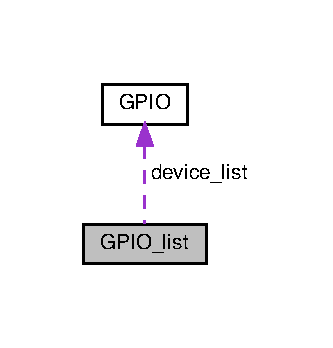
\includegraphics[width=160pt]{structGPIO__list__coll__graph}
\end{center}
\end{figure}
\subsection*{Data Fields}


\subsection{Detailed Description}
Struttura dati per la gestione di più device \hyperlink{structGPIO}{G\+P\+IO} da parte del driver. 

\subsection{Field Documentation}
\mbox{\Hypertarget{structGPIO__list_a170d1d78f27f6ab4c8badaaa4b3f2305}\label{structGPIO__list_a170d1d78f27f6ab4c8badaaa4b3f2305}} 
\index{G\+P\+I\+O\+\_\+list@{G\+P\+I\+O\+\_\+list}!device\+\_\+count@{device\+\_\+count}}
\index{device\+\_\+count@{device\+\_\+count}!G\+P\+I\+O\+\_\+list@{G\+P\+I\+O\+\_\+list}}
\subsubsection{\texorpdfstring{device\+\_\+count}{device\_count}}
{\footnotesize\ttfamily uint32\+\_\+t device\+\_\+count}

numero di device attivi e gestiti dal driver \mbox{\Hypertarget{structGPIO__list_a1f17219814029f429cd2f3fdf4190e0b}\label{structGPIO__list_a1f17219814029f429cd2f3fdf4190e0b}} 
\index{G\+P\+I\+O\+\_\+list@{G\+P\+I\+O\+\_\+list}!device\+\_\+list@{device\+\_\+list}}
\index{device\+\_\+list@{device\+\_\+list}!G\+P\+I\+O\+\_\+list@{G\+P\+I\+O\+\_\+list}}
\subsubsection{\texorpdfstring{device\+\_\+list}{device\_list}}
{\footnotesize\ttfamily \hyperlink{structGPIO}{G\+P\+IO}$\ast$$\ast$ device\+\_\+list}

array di puntatori a \hyperlink{structGPIO}{G\+P\+IO}, ciascuno dei quali si riferisce ad un device \mbox{\Hypertarget{structGPIO__list_aeff61809685e5df1b38aec1d871a49bb}\label{structGPIO__list_aeff61809685e5df1b38aec1d871a49bb}} 
\index{G\+P\+I\+O\+\_\+list@{G\+P\+I\+O\+\_\+list}!list\+\_\+size@{list\+\_\+size}}
\index{list\+\_\+size@{list\+\_\+size}!G\+P\+I\+O\+\_\+list@{G\+P\+I\+O\+\_\+list}}
\subsubsection{\texorpdfstring{list\+\_\+size}{list\_size}}
{\footnotesize\ttfamily uint32\+\_\+t list\+\_\+size}

dimensione della lista, ovvero il numero massimo di device gestibili 

The documentation for this struct was generated from the following file\+:\begin{DoxyCompactItemize}
\item 
/media/saverio/\+O\+S/\+Users/\+Saverio/\+Desktop/\+S\+E/git/codici\+\_\+da\+\_\+mandare/\+F\+P\+G\+A/\+G\+P\+I\+O/\+Driver/\+Kernel\+\_\+\+Mode/\hyperlink{GPIO__list_8h}{G\+P\+I\+O\+\_\+list.\+h}\end{DoxyCompactItemize}

\hypertarget{classGPIO__v1__0}{}\section{G\+P\+I\+O\+\_\+v1\+\_\+0 Entity Reference}
\label{classGPIO__v1__0}\index{G\+P\+I\+O\+\_\+v1\+\_\+0@{G\+P\+I\+O\+\_\+v1\+\_\+0}}


Inheritance diagram for G\+P\+I\+O\+\_\+v1\+\_\+0\+:\nopagebreak
\begin{figure}[H]
\begin{center}
\leavevmode
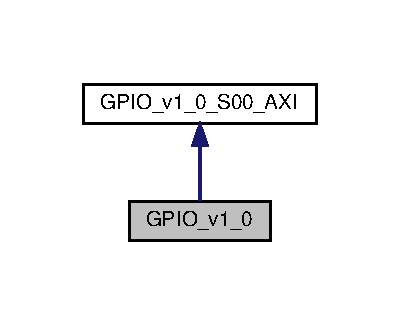
\includegraphics[width=192pt]{classGPIO__v1__0__inherit__graph}
\end{center}
\end{figure}


Collaboration diagram for G\+P\+I\+O\+\_\+v1\+\_\+0\+:\nopagebreak
\begin{figure}[H]
\begin{center}
\leavevmode
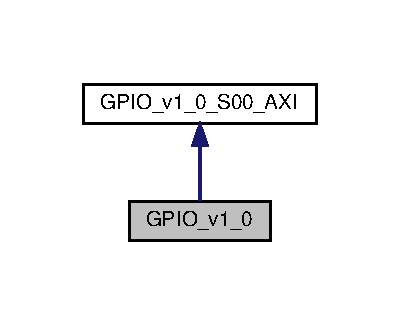
\includegraphics[width=192pt]{classGPIO__v1__0__coll__graph}
\end{center}
\end{figure}
\subsection*{Entities}
\begin{DoxyCompactItemize}
\item 
\hyperlink{classGPIO__v1__0_1_1arch__imp}{arch\+\_\+imp} architecture
\end{DoxyCompactItemize}
\subsection*{Libraries}
 \begin{DoxyCompactItemize}
\item 
\mbox{\Hypertarget{classGPIO__v1__0_a0a6af6eef40212dbaf130d57ce711256}\label{classGPIO__v1__0_a0a6af6eef40212dbaf130d57ce711256}} 
\hyperlink{classGPIO__v1__0_a0a6af6eef40212dbaf130d57ce711256}{ieee} 
\begin{DoxyCompactList}\small\item\em Viene utilizzata la libreria I\+E\+EE. \end{DoxyCompactList}\end{DoxyCompactItemize}
\subsection*{Use Clauses}
 \begin{DoxyCompactItemize}
\item 
\mbox{\Hypertarget{classGPIO__v1__0_acd03516902501cd1c7296a98e22c6fcb}\label{classGPIO__v1__0_acd03516902501cd1c7296a98e22c6fcb}} 
\hyperlink{classGPIO__v1__0_acd03516902501cd1c7296a98e22c6fcb}{std\+\_\+logic\+\_\+1164}   
\begin{DoxyCompactList}\small\item\em Sono utilizzati i segnali della standard logic. \end{DoxyCompactList}\item 
\mbox{\Hypertarget{classGPIO__v1__0_a2edc34402b573437d5f25fa90ba4013e}\label{classGPIO__v1__0_a2edc34402b573437d5f25fa90ba4013e}} 
\hyperlink{classGPIO__v1__0_a2edc34402b573437d5f25fa90ba4013e}{numeric\+\_\+std}   
\begin{DoxyCompactList}\small\item\em Vengono utilizzate le funzioni numeriche. \end{DoxyCompactList}\end{DoxyCompactItemize}
\subsection*{Generics}
 \begin{DoxyCompactItemize}
\item 
\mbox{\Hypertarget{classGPIO__v1__0_a16bbf9205afa677edb8a74dcd39ebb9f}\label{classGPIO__v1__0_a16bbf9205afa677edb8a74dcd39ebb9f}} 
\hyperlink{classGPIO__v1__0_a16bbf9205afa677edb8a74dcd39ebb9f}{width} {\bfseries {\bfseries \textcolor{vhdlchar}{integer}\textcolor{vhdlchar}{ }\textcolor{vhdlchar}{ }\textcolor{vhdlchar}{\+:}\textcolor{vhdlchar}{=}\textcolor{vhdlchar}{ }\textcolor{vhdlchar}{ } \textcolor{vhdldigit}{4} \textcolor{vhdlchar}{ }}}
\begin{DoxyCompactList}\small\item\em determina il numero di \hyperlink{structGPIO}{G\+P\+IO} da controllare \end{DoxyCompactList}\item 
\mbox{\Hypertarget{classGPIO__v1__0_afce7943994a4ddfa81f224225976a4c7}\label{classGPIO__v1__0_afce7943994a4ddfa81f224225976a4c7}} 
\hyperlink{classGPIO__v1__0_afce7943994a4ddfa81f224225976a4c7}{C\+\_\+\+S00\+\_\+\+A\+X\+I\+\_\+\+D\+A\+T\+A\+\_\+\+W\+I\+D\+TH} {\bfseries {\bfseries \textcolor{vhdlchar}{integer}\textcolor{vhdlchar}{ }\textcolor{vhdlchar}{ }\textcolor{vhdlchar}{\+:}\textcolor{vhdlchar}{=}\textcolor{vhdlchar}{ }\textcolor{vhdlchar}{ } \textcolor{vhdldigit}{32} \textcolor{vhdlchar}{ }}}
\item 
\mbox{\Hypertarget{classGPIO__v1__0_ab7787f274c76bb896ac98fdcfb570c65}\label{classGPIO__v1__0_ab7787f274c76bb896ac98fdcfb570c65}} 
\hyperlink{classGPIO__v1__0_ab7787f274c76bb896ac98fdcfb570c65}{C\+\_\+\+S00\+\_\+\+A\+X\+I\+\_\+\+A\+D\+D\+R\+\_\+\+W\+I\+D\+TH} {\bfseries {\bfseries \textcolor{vhdlchar}{integer}\textcolor{vhdlchar}{ }\textcolor{vhdlchar}{ }\textcolor{vhdlchar}{\+:}\textcolor{vhdlchar}{=}\textcolor{vhdlchar}{ }\textcolor{vhdlchar}{ } \textcolor{vhdldigit}{5} \textcolor{vhdlchar}{ }}}
\end{DoxyCompactItemize}
\subsection*{Ports}
 \begin{DoxyCompactItemize}
\item 
\mbox{\Hypertarget{classGPIO__v1__0_ac0744a550c27f11ab186fd7a1156a54e}\label{classGPIO__v1__0_ac0744a550c27f11ab186fd7a1156a54e}} 
\hyperlink{classGPIO__v1__0_ac0744a550c27f11ab186fd7a1156a54e}{pads}  {\bfseries {\bfseries \textcolor{vhdlchar}{inout}\textcolor{vhdlchar}{ }}} {\bfseries \textcolor{vhdlchar}{std\+\_\+logic\+\_\+vector}\textcolor{vhdlchar}{ }\textcolor{vhdlchar}{(}\textcolor{vhdlchar}{ }\textcolor{vhdlchar}{ }\textcolor{vhdlchar}{ }\textcolor{vhdlchar}{ }{\bfseries \hyperlink{classGPIO__v1__0_a16bbf9205afa677edb8a74dcd39ebb9f}{width}} \textcolor{vhdlchar}{-\/}\textcolor{vhdlchar}{ } \textcolor{vhdldigit}{1} \textcolor{vhdlchar}{ }\textcolor{vhdlchar}{downto}\textcolor{vhdlchar}{ }\textcolor{vhdlchar}{ } \textcolor{vhdldigit}{0} \textcolor{vhdlchar}{ }\textcolor{vhdlchar}{)}\textcolor{vhdlchar}{ }} 
\begin{DoxyCompactList}\small\item\em se \hyperlink{structGPIO}{G\+P\+IO} in modalità lettura mostra il valore letto, altrimenti forza un valore in uscita \end{DoxyCompactList}\item 
\mbox{\Hypertarget{classGPIO__v1__0_a5b78f3e3edfaf6e8ec79031b9e631e9d}\label{classGPIO__v1__0_a5b78f3e3edfaf6e8ec79031b9e631e9d}} 
\hyperlink{classGPIO__v1__0_a5b78f3e3edfaf6e8ec79031b9e631e9d}{interrupt}  {\bfseries {\bfseries \textcolor{vhdlchar}{out}\textcolor{vhdlchar}{ }}} {\bfseries \textcolor{vhdlchar}{std\+\_\+logic}\textcolor{vhdlchar}{ }} 
\begin{DoxyCompactList}\small\item\em segnale di interrupt \end{DoxyCompactList}\item 
\mbox{\Hypertarget{classGPIO__v1__0_a037f9e3df8559bfd59db37bcba9cb7a8}\label{classGPIO__v1__0_a037f9e3df8559bfd59db37bcba9cb7a8}} 
\hyperlink{classGPIO__v1__0_a037f9e3df8559bfd59db37bcba9cb7a8}{s00\+\_\+axi\+\_\+aclk}  {\bfseries {\bfseries \textcolor{vhdlchar}{in}\textcolor{vhdlchar}{ }}} {\bfseries \textcolor{vhdlchar}{std\+\_\+logic}\textcolor{vhdlchar}{ }} 
\item 
\mbox{\Hypertarget{classGPIO__v1__0_a8249c106fbd80196dcad2666c9f0b3fc}\label{classGPIO__v1__0_a8249c106fbd80196dcad2666c9f0b3fc}} 
\hyperlink{classGPIO__v1__0_a8249c106fbd80196dcad2666c9f0b3fc}{s00\+\_\+axi\+\_\+aresetn}  {\bfseries {\bfseries \textcolor{vhdlchar}{in}\textcolor{vhdlchar}{ }}} {\bfseries \textcolor{vhdlchar}{std\+\_\+logic}\textcolor{vhdlchar}{ }} 
\item 
\mbox{\Hypertarget{classGPIO__v1__0_a9fe80d3cc7f862afb670536e4e05dbeb}\label{classGPIO__v1__0_a9fe80d3cc7f862afb670536e4e05dbeb}} 
\hyperlink{classGPIO__v1__0_a9fe80d3cc7f862afb670536e4e05dbeb}{s00\+\_\+axi\+\_\+awaddr}  {\bfseries {\bfseries \textcolor{vhdlchar}{in}\textcolor{vhdlchar}{ }}} {\bfseries \textcolor{vhdlchar}{std\+\_\+logic\+\_\+vector}\textcolor{vhdlchar}{ }\textcolor{vhdlchar}{(}\textcolor{vhdlchar}{ }\textcolor{vhdlchar}{ }\textcolor{vhdlchar}{ }\textcolor{vhdlchar}{ }\textcolor{vhdlchar}{C\+\_\+\+S00\+\_\+\+A\+X\+I\+\_\+\+A\+D\+D\+R\+\_\+\+W\+I\+D\+TH}\textcolor{vhdlchar}{-\/}\textcolor{vhdlchar}{ } \textcolor{vhdldigit}{1} \textcolor{vhdlchar}{ }\textcolor{vhdlchar}{downto}\textcolor{vhdlchar}{ }\textcolor{vhdlchar}{ } \textcolor{vhdldigit}{0} \textcolor{vhdlchar}{ }\textcolor{vhdlchar}{)}\textcolor{vhdlchar}{ }} 
\item 
\mbox{\Hypertarget{classGPIO__v1__0_a719659c1addef5432978cc949d9e10ed}\label{classGPIO__v1__0_a719659c1addef5432978cc949d9e10ed}} 
\hyperlink{classGPIO__v1__0_a719659c1addef5432978cc949d9e10ed}{s00\+\_\+axi\+\_\+awprot}  {\bfseries {\bfseries \textcolor{vhdlchar}{in}\textcolor{vhdlchar}{ }}} {\bfseries \textcolor{vhdlchar}{std\+\_\+logic\+\_\+vector}\textcolor{vhdlchar}{ }\textcolor{vhdlchar}{(}\textcolor{vhdlchar}{ }\textcolor{vhdlchar}{ } \textcolor{vhdldigit}{2} \textcolor{vhdlchar}{ }\textcolor{vhdlchar}{downto}\textcolor{vhdlchar}{ }\textcolor{vhdlchar}{ } \textcolor{vhdldigit}{0} \textcolor{vhdlchar}{ }\textcolor{vhdlchar}{)}\textcolor{vhdlchar}{ }} 
\item 
\mbox{\Hypertarget{classGPIO__v1__0_a45aa02a72ae1a8389346d47173c60ed0}\label{classGPIO__v1__0_a45aa02a72ae1a8389346d47173c60ed0}} 
\hyperlink{classGPIO__v1__0_a45aa02a72ae1a8389346d47173c60ed0}{s00\+\_\+axi\+\_\+awvalid}  {\bfseries {\bfseries \textcolor{vhdlchar}{in}\textcolor{vhdlchar}{ }}} {\bfseries \textcolor{vhdlchar}{std\+\_\+logic}\textcolor{vhdlchar}{ }} 
\item 
\mbox{\Hypertarget{classGPIO__v1__0_ad0a1f71502d91a45dbc6c365f85c6566}\label{classGPIO__v1__0_ad0a1f71502d91a45dbc6c365f85c6566}} 
\hyperlink{classGPIO__v1__0_ad0a1f71502d91a45dbc6c365f85c6566}{s00\+\_\+axi\+\_\+awready}  {\bfseries {\bfseries \textcolor{vhdlchar}{out}\textcolor{vhdlchar}{ }}} {\bfseries \textcolor{vhdlchar}{std\+\_\+logic}\textcolor{vhdlchar}{ }} 
\item 
\mbox{\Hypertarget{classGPIO__v1__0_ae2b15b55ee463fd9dd030ee29db6bb17}\label{classGPIO__v1__0_ae2b15b55ee463fd9dd030ee29db6bb17}} 
\hyperlink{classGPIO__v1__0_ae2b15b55ee463fd9dd030ee29db6bb17}{s00\+\_\+axi\+\_\+wdata}  {\bfseries {\bfseries \textcolor{vhdlchar}{in}\textcolor{vhdlchar}{ }}} {\bfseries \textcolor{vhdlchar}{std\+\_\+logic\+\_\+vector}\textcolor{vhdlchar}{ }\textcolor{vhdlchar}{(}\textcolor{vhdlchar}{ }\textcolor{vhdlchar}{ }\textcolor{vhdlchar}{ }\textcolor{vhdlchar}{ }\textcolor{vhdlchar}{C\+\_\+\+S00\+\_\+\+A\+X\+I\+\_\+\+D\+A\+T\+A\+\_\+\+W\+I\+D\+TH}\textcolor{vhdlchar}{-\/}\textcolor{vhdlchar}{ } \textcolor{vhdldigit}{1} \textcolor{vhdlchar}{ }\textcolor{vhdlchar}{downto}\textcolor{vhdlchar}{ }\textcolor{vhdlchar}{ } \textcolor{vhdldigit}{0} \textcolor{vhdlchar}{ }\textcolor{vhdlchar}{)}\textcolor{vhdlchar}{ }} 
\item 
\mbox{\Hypertarget{classGPIO__v1__0_a120924bc3fd5fd10ec0f96e19c3f4904}\label{classGPIO__v1__0_a120924bc3fd5fd10ec0f96e19c3f4904}} 
\hyperlink{classGPIO__v1__0_a120924bc3fd5fd10ec0f96e19c3f4904}{s00\+\_\+axi\+\_\+wstrb}  {\bfseries {\bfseries \textcolor{vhdlchar}{in}\textcolor{vhdlchar}{ }}} {\bfseries \textcolor{vhdlchar}{std\+\_\+logic\+\_\+vector}\textcolor{vhdlchar}{ }\textcolor{vhdlchar}{(}\textcolor{vhdlchar}{ }\textcolor{vhdlchar}{(}\textcolor{vhdlchar}{ }\textcolor{vhdlchar}{ }\textcolor{vhdlchar}{ }\textcolor{vhdlchar}{ }\textcolor{vhdlchar}{C\+\_\+\+S00\+\_\+\+A\+X\+I\+\_\+\+D\+A\+T\+A\+\_\+\+W\+I\+D\+TH}\textcolor{vhdlchar}{/}\textcolor{vhdlchar}{ } \textcolor{vhdldigit}{8} \textcolor{vhdlchar}{ }\textcolor{vhdlchar}{)}\textcolor{vhdlchar}{ }\textcolor{vhdlchar}{-\/}\textcolor{vhdlchar}{ } \textcolor{vhdldigit}{1} \textcolor{vhdlchar}{ }\textcolor{vhdlchar}{downto}\textcolor{vhdlchar}{ }\textcolor{vhdlchar}{ } \textcolor{vhdldigit}{0} \textcolor{vhdlchar}{ }\textcolor{vhdlchar}{)}\textcolor{vhdlchar}{ }} 
\item 
\mbox{\Hypertarget{classGPIO__v1__0_a24e90907193647007d2947353740114d}\label{classGPIO__v1__0_a24e90907193647007d2947353740114d}} 
\hyperlink{classGPIO__v1__0_a24e90907193647007d2947353740114d}{s00\+\_\+axi\+\_\+wvalid}  {\bfseries {\bfseries \textcolor{vhdlchar}{in}\textcolor{vhdlchar}{ }}} {\bfseries \textcolor{vhdlchar}{std\+\_\+logic}\textcolor{vhdlchar}{ }} 
\item 
\mbox{\Hypertarget{classGPIO__v1__0_a3fc60abc0cfbfa90003a83bffdd476c4}\label{classGPIO__v1__0_a3fc60abc0cfbfa90003a83bffdd476c4}} 
\hyperlink{classGPIO__v1__0_a3fc60abc0cfbfa90003a83bffdd476c4}{s00\+\_\+axi\+\_\+wready}  {\bfseries {\bfseries \textcolor{vhdlchar}{out}\textcolor{vhdlchar}{ }}} {\bfseries \textcolor{vhdlchar}{std\+\_\+logic}\textcolor{vhdlchar}{ }} 
\item 
\mbox{\Hypertarget{classGPIO__v1__0_af8799be946d3f5354263e7deb15f94f1}\label{classGPIO__v1__0_af8799be946d3f5354263e7deb15f94f1}} 
\hyperlink{classGPIO__v1__0_af8799be946d3f5354263e7deb15f94f1}{s00\+\_\+axi\+\_\+bresp}  {\bfseries {\bfseries \textcolor{vhdlchar}{out}\textcolor{vhdlchar}{ }}} {\bfseries \textcolor{vhdlchar}{std\+\_\+logic\+\_\+vector}\textcolor{vhdlchar}{ }\textcolor{vhdlchar}{(}\textcolor{vhdlchar}{ }\textcolor{vhdlchar}{ } \textcolor{vhdldigit}{1} \textcolor{vhdlchar}{ }\textcolor{vhdlchar}{downto}\textcolor{vhdlchar}{ }\textcolor{vhdlchar}{ } \textcolor{vhdldigit}{0} \textcolor{vhdlchar}{ }\textcolor{vhdlchar}{)}\textcolor{vhdlchar}{ }} 
\item 
\mbox{\Hypertarget{classGPIO__v1__0_a5110b7dd4fb9548a2aab88f50dbe1d5e}\label{classGPIO__v1__0_a5110b7dd4fb9548a2aab88f50dbe1d5e}} 
\hyperlink{classGPIO__v1__0_a5110b7dd4fb9548a2aab88f50dbe1d5e}{s00\+\_\+axi\+\_\+bvalid}  {\bfseries {\bfseries \textcolor{vhdlchar}{out}\textcolor{vhdlchar}{ }}} {\bfseries \textcolor{vhdlchar}{std\+\_\+logic}\textcolor{vhdlchar}{ }} 
\item 
\mbox{\Hypertarget{classGPIO__v1__0_a1ef2019b0613bc23d4829eeeb24eb98d}\label{classGPIO__v1__0_a1ef2019b0613bc23d4829eeeb24eb98d}} 
\hyperlink{classGPIO__v1__0_a1ef2019b0613bc23d4829eeeb24eb98d}{s00\+\_\+axi\+\_\+bready}  {\bfseries {\bfseries \textcolor{vhdlchar}{in}\textcolor{vhdlchar}{ }}} {\bfseries \textcolor{vhdlchar}{std\+\_\+logic}\textcolor{vhdlchar}{ }} 
\item 
\mbox{\Hypertarget{classGPIO__v1__0_af70a86336cd6505064e45b69f4623939}\label{classGPIO__v1__0_af70a86336cd6505064e45b69f4623939}} 
\hyperlink{classGPIO__v1__0_af70a86336cd6505064e45b69f4623939}{s00\+\_\+axi\+\_\+araddr}  {\bfseries {\bfseries \textcolor{vhdlchar}{in}\textcolor{vhdlchar}{ }}} {\bfseries \textcolor{vhdlchar}{std\+\_\+logic\+\_\+vector}\textcolor{vhdlchar}{ }\textcolor{vhdlchar}{(}\textcolor{vhdlchar}{ }\textcolor{vhdlchar}{ }\textcolor{vhdlchar}{ }\textcolor{vhdlchar}{ }\textcolor{vhdlchar}{C\+\_\+\+S00\+\_\+\+A\+X\+I\+\_\+\+A\+D\+D\+R\+\_\+\+W\+I\+D\+TH}\textcolor{vhdlchar}{-\/}\textcolor{vhdlchar}{ } \textcolor{vhdldigit}{1} \textcolor{vhdlchar}{ }\textcolor{vhdlchar}{downto}\textcolor{vhdlchar}{ }\textcolor{vhdlchar}{ } \textcolor{vhdldigit}{0} \textcolor{vhdlchar}{ }\textcolor{vhdlchar}{)}\textcolor{vhdlchar}{ }} 
\item 
\mbox{\Hypertarget{classGPIO__v1__0_adc648df07895bf808b8c721e1dc6811b}\label{classGPIO__v1__0_adc648df07895bf808b8c721e1dc6811b}} 
\hyperlink{classGPIO__v1__0_adc648df07895bf808b8c721e1dc6811b}{s00\+\_\+axi\+\_\+arprot}  {\bfseries {\bfseries \textcolor{vhdlchar}{in}\textcolor{vhdlchar}{ }}} {\bfseries \textcolor{vhdlchar}{std\+\_\+logic\+\_\+vector}\textcolor{vhdlchar}{ }\textcolor{vhdlchar}{(}\textcolor{vhdlchar}{ }\textcolor{vhdlchar}{ } \textcolor{vhdldigit}{2} \textcolor{vhdlchar}{ }\textcolor{vhdlchar}{downto}\textcolor{vhdlchar}{ }\textcolor{vhdlchar}{ } \textcolor{vhdldigit}{0} \textcolor{vhdlchar}{ }\textcolor{vhdlchar}{)}\textcolor{vhdlchar}{ }} 
\item 
\mbox{\Hypertarget{classGPIO__v1__0_a94b78b2ae3cd13860f15afbdfb199e44}\label{classGPIO__v1__0_a94b78b2ae3cd13860f15afbdfb199e44}} 
\hyperlink{classGPIO__v1__0_a94b78b2ae3cd13860f15afbdfb199e44}{s00\+\_\+axi\+\_\+arvalid}  {\bfseries {\bfseries \textcolor{vhdlchar}{in}\textcolor{vhdlchar}{ }}} {\bfseries \textcolor{vhdlchar}{std\+\_\+logic}\textcolor{vhdlchar}{ }} 
\item 
\mbox{\Hypertarget{classGPIO__v1__0_ad35bd95f3352ff8dbdaea55205a98e53}\label{classGPIO__v1__0_ad35bd95f3352ff8dbdaea55205a98e53}} 
\hyperlink{classGPIO__v1__0_ad35bd95f3352ff8dbdaea55205a98e53}{s00\+\_\+axi\+\_\+arready}  {\bfseries {\bfseries \textcolor{vhdlchar}{out}\textcolor{vhdlchar}{ }}} {\bfseries \textcolor{vhdlchar}{std\+\_\+logic}\textcolor{vhdlchar}{ }} 
\item 
\mbox{\Hypertarget{classGPIO__v1__0_ad2655fadb987e0487c428aca187b55d0}\label{classGPIO__v1__0_ad2655fadb987e0487c428aca187b55d0}} 
\hyperlink{classGPIO__v1__0_ad2655fadb987e0487c428aca187b55d0}{s00\+\_\+axi\+\_\+rdata}  {\bfseries {\bfseries \textcolor{vhdlchar}{out}\textcolor{vhdlchar}{ }}} {\bfseries \textcolor{vhdlchar}{std\+\_\+logic\+\_\+vector}\textcolor{vhdlchar}{ }\textcolor{vhdlchar}{(}\textcolor{vhdlchar}{ }\textcolor{vhdlchar}{ }\textcolor{vhdlchar}{ }\textcolor{vhdlchar}{ }\textcolor{vhdlchar}{C\+\_\+\+S00\+\_\+\+A\+X\+I\+\_\+\+D\+A\+T\+A\+\_\+\+W\+I\+D\+TH}\textcolor{vhdlchar}{-\/}\textcolor{vhdlchar}{ } \textcolor{vhdldigit}{1} \textcolor{vhdlchar}{ }\textcolor{vhdlchar}{downto}\textcolor{vhdlchar}{ }\textcolor{vhdlchar}{ } \textcolor{vhdldigit}{0} \textcolor{vhdlchar}{ }\textcolor{vhdlchar}{)}\textcolor{vhdlchar}{ }} 
\item 
\mbox{\Hypertarget{classGPIO__v1__0_a1acee955f50f71e5595a03c6ca301cf0}\label{classGPIO__v1__0_a1acee955f50f71e5595a03c6ca301cf0}} 
\hyperlink{classGPIO__v1__0_a1acee955f50f71e5595a03c6ca301cf0}{s00\+\_\+axi\+\_\+rresp}  {\bfseries {\bfseries \textcolor{vhdlchar}{out}\textcolor{vhdlchar}{ }}} {\bfseries \textcolor{vhdlchar}{std\+\_\+logic\+\_\+vector}\textcolor{vhdlchar}{ }\textcolor{vhdlchar}{(}\textcolor{vhdlchar}{ }\textcolor{vhdlchar}{ } \textcolor{vhdldigit}{1} \textcolor{vhdlchar}{ }\textcolor{vhdlchar}{downto}\textcolor{vhdlchar}{ }\textcolor{vhdlchar}{ } \textcolor{vhdldigit}{0} \textcolor{vhdlchar}{ }\textcolor{vhdlchar}{)}\textcolor{vhdlchar}{ }} 
\item 
\mbox{\Hypertarget{classGPIO__v1__0_af180911f7eb262e530e26865bc97aa0b}\label{classGPIO__v1__0_af180911f7eb262e530e26865bc97aa0b}} 
\hyperlink{classGPIO__v1__0_af180911f7eb262e530e26865bc97aa0b}{s00\+\_\+axi\+\_\+rvalid}  {\bfseries {\bfseries \textcolor{vhdlchar}{out}\textcolor{vhdlchar}{ }}} {\bfseries \textcolor{vhdlchar}{std\+\_\+logic}\textcolor{vhdlchar}{ }} 
\item 
\mbox{\Hypertarget{classGPIO__v1__0_a8b82eb165d7024f6c7b25646f6ebdd4d}\label{classGPIO__v1__0_a8b82eb165d7024f6c7b25646f6ebdd4d}} 
\hyperlink{classGPIO__v1__0_a8b82eb165d7024f6c7b25646f6ebdd4d}{s00\+\_\+axi\+\_\+rready}  {\bfseries {\bfseries \textcolor{vhdlchar}{in}\textcolor{vhdlchar}{ }}} {\bfseries \textcolor{vhdlchar}{std\+\_\+logic}\textcolor{vhdlchar}{ }} 
\end{DoxyCompactItemize}


The documentation for this class was generated from the following file\+:\begin{DoxyCompactItemize}
\item 
/media/saverio/\+O\+S/\+Users/\+Saverio/\+Desktop/\+S\+E/git/codici\+\_\+da\+\_\+mandare/\+F\+P\+G\+A/\+G\+P\+I\+O/\+Hardware/\+G\+P\+I\+O\+\_\+1.\+0/hdl/\hyperlink{GPIO__v1__0_8vhd}{G\+P\+I\+O\+\_\+v1\+\_\+0.\+vhd}\end{DoxyCompactItemize}

\hypertarget{classGPIO__v1__0__S00__AXI}{}\section{G\+P\+I\+O\+\_\+v1\+\_\+0\+\_\+\+S00\+\_\+\+A\+XI Entity Reference}
\label{classGPIO__v1__0__S00__AXI}\index{G\+P\+I\+O\+\_\+v1\+\_\+0\+\_\+\+S00\+\_\+\+A\+XI@{G\+P\+I\+O\+\_\+v1\+\_\+0\+\_\+\+S00\+\_\+\+A\+XI}}


Inheritance diagram for G\+P\+I\+O\+\_\+v1\+\_\+0\+\_\+\+S00\+\_\+\+A\+XI\+:\nopagebreak
\begin{figure}[H]
\begin{center}
\leavevmode
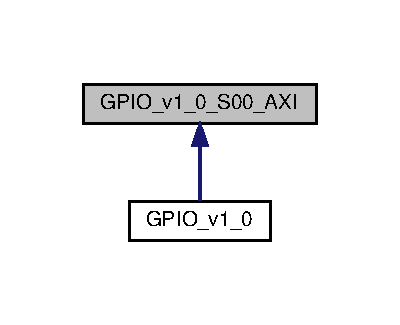
\includegraphics[width=192pt]{classGPIO__v1__0__S00__AXI__inherit__graph}
\end{center}
\end{figure}
\subsection*{Entities}
\begin{DoxyCompactItemize}
\item 
\hyperlink{classGPIO__v1__0__S00__AXI_1_1arch__imp}{arch\+\_\+imp} architecture
\end{DoxyCompactItemize}
\subsection*{Libraries}
 \begin{DoxyCompactItemize}
\item 
\mbox{\Hypertarget{classGPIO__v1__0__S00__AXI_a0a6af6eef40212dbaf130d57ce711256}\label{classGPIO__v1__0__S00__AXI_a0a6af6eef40212dbaf130d57ce711256}} 
\hyperlink{classGPIO__v1__0__S00__AXI_a0a6af6eef40212dbaf130d57ce711256}{ieee} 
\begin{DoxyCompactList}\small\item\em Viene utilizzato la libreria I\+E\+EE. \end{DoxyCompactList}\end{DoxyCompactItemize}
\subsection*{Use Clauses}
 \begin{DoxyCompactItemize}
\item 
\mbox{\Hypertarget{classGPIO__v1__0__S00__AXI_acd03516902501cd1c7296a98e22c6fcb}\label{classGPIO__v1__0__S00__AXI_acd03516902501cd1c7296a98e22c6fcb}} 
\hyperlink{classGPIO__v1__0__S00__AXI_acd03516902501cd1c7296a98e22c6fcb}{std\+\_\+logic\+\_\+1164}   
\begin{DoxyCompactList}\small\item\em Sono utilizzati i segnali della standard logic. \end{DoxyCompactList}\item 
\mbox{\Hypertarget{classGPIO__v1__0__S00__AXI_a2edc34402b573437d5f25fa90ba4013e}\label{classGPIO__v1__0__S00__AXI_a2edc34402b573437d5f25fa90ba4013e}} 
\hyperlink{classGPIO__v1__0__S00__AXI_a2edc34402b573437d5f25fa90ba4013e}{numeric\+\_\+std}   
\begin{DoxyCompactList}\small\item\em Vengono utilizzate le funzioni numeriche. \end{DoxyCompactList}\item 
\mbox{\Hypertarget{classGPIO__v1__0__S00__AXI_acb2d98d781f19c8f5f4109576ec45502}\label{classGPIO__v1__0__S00__AXI_acb2d98d781f19c8f5f4109576ec45502}} 
\hyperlink{classGPIO__v1__0__S00__AXI_acb2d98d781f19c8f5f4109576ec45502}{std\+\_\+logic\+\_\+misc}   
\begin{DoxyCompactList}\small\item\em Viene utilizzata la libreria misc di utility. \end{DoxyCompactList}\end{DoxyCompactItemize}
\subsection*{Generics}
 \begin{DoxyCompactItemize}
\item 
\mbox{\Hypertarget{classGPIO__v1__0__S00__AXI_a16bbf9205afa677edb8a74dcd39ebb9f}\label{classGPIO__v1__0__S00__AXI_a16bbf9205afa677edb8a74dcd39ebb9f}} 
\hyperlink{classGPIO__v1__0__S00__AXI_a16bbf9205afa677edb8a74dcd39ebb9f}{width} {\bfseries {\bfseries \textcolor{vhdlchar}{integer}\textcolor{vhdlchar}{ }\textcolor{vhdlchar}{ }\textcolor{vhdlchar}{\+:}\textcolor{vhdlchar}{=}\textcolor{vhdlchar}{ }\textcolor{vhdlchar}{ } \textcolor{vhdldigit}{4} \textcolor{vhdlchar}{ }}}
\begin{DoxyCompactList}\small\item\em determina il numero di \hyperlink{structGPIO}{G\+P\+IO} da controllare \end{DoxyCompactList}\item 
\mbox{\Hypertarget{classGPIO__v1__0__S00__AXI_a0fad312acd1f302ce7de30c5658df0bd}\label{classGPIO__v1__0__S00__AXI_a0fad312acd1f302ce7de30c5658df0bd}} 
\hyperlink{classGPIO__v1__0__S00__AXI_a0fad312acd1f302ce7de30c5658df0bd}{C\+\_\+\+S\+\_\+\+A\+X\+I\+\_\+\+D\+A\+T\+A\+\_\+\+W\+I\+D\+TH} {\bfseries {\bfseries \textcolor{vhdlchar}{integer}\textcolor{vhdlchar}{ }\textcolor{vhdlchar}{ }\textcolor{vhdlchar}{\+:}\textcolor{vhdlchar}{=}\textcolor{vhdlchar}{ }\textcolor{vhdlchar}{ } \textcolor{vhdldigit}{32} \textcolor{vhdlchar}{ }}}
\item 
\mbox{\Hypertarget{classGPIO__v1__0__S00__AXI_a9abff2eaa069440f3b7d9e9937d5ee8e}\label{classGPIO__v1__0__S00__AXI_a9abff2eaa069440f3b7d9e9937d5ee8e}} 
\hyperlink{classGPIO__v1__0__S00__AXI_a9abff2eaa069440f3b7d9e9937d5ee8e}{C\+\_\+\+S\+\_\+\+A\+X\+I\+\_\+\+A\+D\+D\+R\+\_\+\+W\+I\+D\+TH} {\bfseries {\bfseries \textcolor{vhdlchar}{integer}\textcolor{vhdlchar}{ }\textcolor{vhdlchar}{ }\textcolor{vhdlchar}{\+:}\textcolor{vhdlchar}{=}\textcolor{vhdlchar}{ }\textcolor{vhdlchar}{ } \textcolor{vhdldigit}{5} \textcolor{vhdlchar}{ }}}
\end{DoxyCompactItemize}
\subsection*{Ports}
 \begin{DoxyCompactItemize}
\item 
\mbox{\Hypertarget{classGPIO__v1__0__S00__AXI_ac0744a550c27f11ab186fd7a1156a54e}\label{classGPIO__v1__0__S00__AXI_ac0744a550c27f11ab186fd7a1156a54e}} 
\hyperlink{classGPIO__v1__0__S00__AXI_ac0744a550c27f11ab186fd7a1156a54e}{pads}  {\bfseries {\bfseries \textcolor{vhdlchar}{inout}\textcolor{vhdlchar}{ }}} {\bfseries \textcolor{vhdlchar}{std\+\_\+logic\+\_\+vector}\textcolor{vhdlchar}{ }\textcolor{vhdlchar}{(}\textcolor{vhdlchar}{ }\textcolor{vhdlchar}{ }\textcolor{vhdlchar}{ }\textcolor{vhdlchar}{ }{\bfseries \hyperlink{classGPIO__v1__0__S00__AXI_a16bbf9205afa677edb8a74dcd39ebb9f}{width}} \textcolor{vhdlchar}{-\/}\textcolor{vhdlchar}{ } \textcolor{vhdldigit}{1} \textcolor{vhdlchar}{ }\textcolor{vhdlchar}{downto}\textcolor{vhdlchar}{ }\textcolor{vhdlchar}{ } \textcolor{vhdldigit}{0} \textcolor{vhdlchar}{ }\textcolor{vhdlchar}{)}\textcolor{vhdlchar}{ }} 
\begin{DoxyCompactList}\small\item\em se \hyperlink{structGPIO}{G\+P\+IO} in modalità lettura mostra il valore letto, altrimenti forza un valore in uscita \end{DoxyCompactList}\item 
\mbox{\Hypertarget{classGPIO__v1__0__S00__AXI_a5b78f3e3edfaf6e8ec79031b9e631e9d}\label{classGPIO__v1__0__S00__AXI_a5b78f3e3edfaf6e8ec79031b9e631e9d}} 
\hyperlink{classGPIO__v1__0__S00__AXI_a5b78f3e3edfaf6e8ec79031b9e631e9d}{interrupt}  {\bfseries {\bfseries \textcolor{vhdlchar}{out}\textcolor{vhdlchar}{ }}} {\bfseries \textcolor{vhdlchar}{std\+\_\+logic}\textcolor{vhdlchar}{ }} 
\begin{DoxyCompactList}\small\item\em segnale di interrupt \end{DoxyCompactList}\item 
\mbox{\Hypertarget{classGPIO__v1__0__S00__AXI_a3f54d782a88290bdaa6baffd7cd84ab4}\label{classGPIO__v1__0__S00__AXI_a3f54d782a88290bdaa6baffd7cd84ab4}} 
\hyperlink{classGPIO__v1__0__S00__AXI_a3f54d782a88290bdaa6baffd7cd84ab4}{S\+\_\+\+A\+X\+I\+\_\+\+A\+C\+LK}  {\bfseries {\bfseries \textcolor{vhdlchar}{in}\textcolor{vhdlchar}{ }}} {\bfseries \textcolor{vhdlchar}{std\+\_\+logic}\textcolor{vhdlchar}{ }} 
\item 
\mbox{\Hypertarget{classGPIO__v1__0__S00__AXI_a089b396e17dee353ccc7d5389dda5532}\label{classGPIO__v1__0__S00__AXI_a089b396e17dee353ccc7d5389dda5532}} 
\hyperlink{classGPIO__v1__0__S00__AXI_a089b396e17dee353ccc7d5389dda5532}{S\+\_\+\+A\+X\+I\+\_\+\+A\+R\+E\+S\+E\+TN}  {\bfseries {\bfseries \textcolor{vhdlchar}{in}\textcolor{vhdlchar}{ }}} {\bfseries \textcolor{vhdlchar}{std\+\_\+logic}\textcolor{vhdlchar}{ }} 
\item 
\mbox{\Hypertarget{classGPIO__v1__0__S00__AXI_a61cc7b190ba9d540e56941330e4a0883}\label{classGPIO__v1__0__S00__AXI_a61cc7b190ba9d540e56941330e4a0883}} 
\hyperlink{classGPIO__v1__0__S00__AXI_a61cc7b190ba9d540e56941330e4a0883}{S\+\_\+\+A\+X\+I\+\_\+\+A\+W\+A\+D\+DR}  {\bfseries {\bfseries \textcolor{vhdlchar}{in}\textcolor{vhdlchar}{ }}} {\bfseries \textcolor{vhdlchar}{std\+\_\+logic\+\_\+vector}\textcolor{vhdlchar}{ }\textcolor{vhdlchar}{(}\textcolor{vhdlchar}{ }\textcolor{vhdlchar}{ }\textcolor{vhdlchar}{ }\textcolor{vhdlchar}{ }\textcolor{vhdlchar}{C\+\_\+\+S\+\_\+\+A\+X\+I\+\_\+\+A\+D\+D\+R\+\_\+\+W\+I\+D\+TH}\textcolor{vhdlchar}{-\/}\textcolor{vhdlchar}{ } \textcolor{vhdldigit}{1} \textcolor{vhdlchar}{ }\textcolor{vhdlchar}{downto}\textcolor{vhdlchar}{ }\textcolor{vhdlchar}{ } \textcolor{vhdldigit}{0} \textcolor{vhdlchar}{ }\textcolor{vhdlchar}{)}\textcolor{vhdlchar}{ }} 
\item 
\mbox{\Hypertarget{classGPIO__v1__0__S00__AXI_a459abcd98567ad24261377eed899593a}\label{classGPIO__v1__0__S00__AXI_a459abcd98567ad24261377eed899593a}} 
\hyperlink{classGPIO__v1__0__S00__AXI_a459abcd98567ad24261377eed899593a}{S\+\_\+\+A\+X\+I\+\_\+\+A\+W\+P\+R\+OT}  {\bfseries {\bfseries \textcolor{vhdlchar}{in}\textcolor{vhdlchar}{ }}} {\bfseries \textcolor{vhdlchar}{std\+\_\+logic\+\_\+vector}\textcolor{vhdlchar}{ }\textcolor{vhdlchar}{(}\textcolor{vhdlchar}{ }\textcolor{vhdlchar}{ } \textcolor{vhdldigit}{2} \textcolor{vhdlchar}{ }\textcolor{vhdlchar}{downto}\textcolor{vhdlchar}{ }\textcolor{vhdlchar}{ } \textcolor{vhdldigit}{0} \textcolor{vhdlchar}{ }\textcolor{vhdlchar}{)}\textcolor{vhdlchar}{ }} 
\item 
\mbox{\Hypertarget{classGPIO__v1__0__S00__AXI_af1f1cbf67bf647ba58353c261719a3a0}\label{classGPIO__v1__0__S00__AXI_af1f1cbf67bf647ba58353c261719a3a0}} 
\hyperlink{classGPIO__v1__0__S00__AXI_af1f1cbf67bf647ba58353c261719a3a0}{S\+\_\+\+A\+X\+I\+\_\+\+A\+W\+V\+A\+L\+ID}  {\bfseries {\bfseries \textcolor{vhdlchar}{in}\textcolor{vhdlchar}{ }}} {\bfseries \textcolor{vhdlchar}{std\+\_\+logic}\textcolor{vhdlchar}{ }} 
\item 
\mbox{\Hypertarget{classGPIO__v1__0__S00__AXI_ac04aab5cc834e762e893e061016921c6}\label{classGPIO__v1__0__S00__AXI_ac04aab5cc834e762e893e061016921c6}} 
\hyperlink{classGPIO__v1__0__S00__AXI_ac04aab5cc834e762e893e061016921c6}{S\+\_\+\+A\+X\+I\+\_\+\+A\+W\+R\+E\+A\+DY}  {\bfseries {\bfseries \textcolor{vhdlchar}{out}\textcolor{vhdlchar}{ }}} {\bfseries \textcolor{vhdlchar}{std\+\_\+logic}\textcolor{vhdlchar}{ }} 
\item 
\mbox{\Hypertarget{classGPIO__v1__0__S00__AXI_a292e5db13719faf3a8b3aab091773467}\label{classGPIO__v1__0__S00__AXI_a292e5db13719faf3a8b3aab091773467}} 
\hyperlink{classGPIO__v1__0__S00__AXI_a292e5db13719faf3a8b3aab091773467}{S\+\_\+\+A\+X\+I\+\_\+\+W\+D\+A\+TA}  {\bfseries {\bfseries \textcolor{vhdlchar}{in}\textcolor{vhdlchar}{ }}} {\bfseries \textcolor{vhdlchar}{std\+\_\+logic\+\_\+vector}\textcolor{vhdlchar}{ }\textcolor{vhdlchar}{(}\textcolor{vhdlchar}{ }\textcolor{vhdlchar}{ }\textcolor{vhdlchar}{ }\textcolor{vhdlchar}{ }\textcolor{vhdlchar}{C\+\_\+\+S\+\_\+\+A\+X\+I\+\_\+\+D\+A\+T\+A\+\_\+\+W\+I\+D\+TH}\textcolor{vhdlchar}{-\/}\textcolor{vhdlchar}{ } \textcolor{vhdldigit}{1} \textcolor{vhdlchar}{ }\textcolor{vhdlchar}{downto}\textcolor{vhdlchar}{ }\textcolor{vhdlchar}{ } \textcolor{vhdldigit}{0} \textcolor{vhdlchar}{ }\textcolor{vhdlchar}{)}\textcolor{vhdlchar}{ }} 
\item 
\mbox{\Hypertarget{classGPIO__v1__0__S00__AXI_accd8e04b79540b57ab15fee1cb6c04f5}\label{classGPIO__v1__0__S00__AXI_accd8e04b79540b57ab15fee1cb6c04f5}} 
\hyperlink{classGPIO__v1__0__S00__AXI_accd8e04b79540b57ab15fee1cb6c04f5}{S\+\_\+\+A\+X\+I\+\_\+\+W\+S\+T\+RB}  {\bfseries {\bfseries \textcolor{vhdlchar}{in}\textcolor{vhdlchar}{ }}} {\bfseries \textcolor{vhdlchar}{std\+\_\+logic\+\_\+vector}\textcolor{vhdlchar}{ }\textcolor{vhdlchar}{(}\textcolor{vhdlchar}{ }\textcolor{vhdlchar}{(}\textcolor{vhdlchar}{ }\textcolor{vhdlchar}{ }\textcolor{vhdlchar}{ }\textcolor{vhdlchar}{ }\textcolor{vhdlchar}{C\+\_\+\+S\+\_\+\+A\+X\+I\+\_\+\+D\+A\+T\+A\+\_\+\+W\+I\+D\+TH}\textcolor{vhdlchar}{/}\textcolor{vhdlchar}{ } \textcolor{vhdldigit}{8} \textcolor{vhdlchar}{ }\textcolor{vhdlchar}{)}\textcolor{vhdlchar}{ }\textcolor{vhdlchar}{-\/}\textcolor{vhdlchar}{ } \textcolor{vhdldigit}{1} \textcolor{vhdlchar}{ }\textcolor{vhdlchar}{downto}\textcolor{vhdlchar}{ }\textcolor{vhdlchar}{ } \textcolor{vhdldigit}{0} \textcolor{vhdlchar}{ }\textcolor{vhdlchar}{)}\textcolor{vhdlchar}{ }} 
\item 
\mbox{\Hypertarget{classGPIO__v1__0__S00__AXI_a60bd882e2de781af9a7c6c3d494225d5}\label{classGPIO__v1__0__S00__AXI_a60bd882e2de781af9a7c6c3d494225d5}} 
\hyperlink{classGPIO__v1__0__S00__AXI_a60bd882e2de781af9a7c6c3d494225d5}{S\+\_\+\+A\+X\+I\+\_\+\+W\+V\+A\+L\+ID}  {\bfseries {\bfseries \textcolor{vhdlchar}{in}\textcolor{vhdlchar}{ }}} {\bfseries \textcolor{vhdlchar}{std\+\_\+logic}\textcolor{vhdlchar}{ }} 
\item 
\mbox{\Hypertarget{classGPIO__v1__0__S00__AXI_ab84e4db7037141a360c2b59f45124f01}\label{classGPIO__v1__0__S00__AXI_ab84e4db7037141a360c2b59f45124f01}} 
\hyperlink{classGPIO__v1__0__S00__AXI_ab84e4db7037141a360c2b59f45124f01}{S\+\_\+\+A\+X\+I\+\_\+\+W\+R\+E\+A\+DY}  {\bfseries {\bfseries \textcolor{vhdlchar}{out}\textcolor{vhdlchar}{ }}} {\bfseries \textcolor{vhdlchar}{std\+\_\+logic}\textcolor{vhdlchar}{ }} 
\item 
\mbox{\Hypertarget{classGPIO__v1__0__S00__AXI_abca6c9777b38a5a6bc04886924bafcc8}\label{classGPIO__v1__0__S00__AXI_abca6c9777b38a5a6bc04886924bafcc8}} 
\hyperlink{classGPIO__v1__0__S00__AXI_abca6c9777b38a5a6bc04886924bafcc8}{S\+\_\+\+A\+X\+I\+\_\+\+B\+R\+E\+SP}  {\bfseries {\bfseries \textcolor{vhdlchar}{out}\textcolor{vhdlchar}{ }}} {\bfseries \textcolor{vhdlchar}{std\+\_\+logic\+\_\+vector}\textcolor{vhdlchar}{ }\textcolor{vhdlchar}{(}\textcolor{vhdlchar}{ }\textcolor{vhdlchar}{ } \textcolor{vhdldigit}{1} \textcolor{vhdlchar}{ }\textcolor{vhdlchar}{downto}\textcolor{vhdlchar}{ }\textcolor{vhdlchar}{ } \textcolor{vhdldigit}{0} \textcolor{vhdlchar}{ }\textcolor{vhdlchar}{)}\textcolor{vhdlchar}{ }} 
\item 
\mbox{\Hypertarget{classGPIO__v1__0__S00__AXI_a58f260d3ebaa69be91bb65ff9211823b}\label{classGPIO__v1__0__S00__AXI_a58f260d3ebaa69be91bb65ff9211823b}} 
\hyperlink{classGPIO__v1__0__S00__AXI_a58f260d3ebaa69be91bb65ff9211823b}{S\+\_\+\+A\+X\+I\+\_\+\+B\+V\+A\+L\+ID}  {\bfseries {\bfseries \textcolor{vhdlchar}{out}\textcolor{vhdlchar}{ }}} {\bfseries \textcolor{vhdlchar}{std\+\_\+logic}\textcolor{vhdlchar}{ }} 
\item 
\mbox{\Hypertarget{classGPIO__v1__0__S00__AXI_ac265989978a2be832d278f63fc0f06cb}\label{classGPIO__v1__0__S00__AXI_ac265989978a2be832d278f63fc0f06cb}} 
\hyperlink{classGPIO__v1__0__S00__AXI_ac265989978a2be832d278f63fc0f06cb}{S\+\_\+\+A\+X\+I\+\_\+\+B\+R\+E\+A\+DY}  {\bfseries {\bfseries \textcolor{vhdlchar}{in}\textcolor{vhdlchar}{ }}} {\bfseries \textcolor{vhdlchar}{std\+\_\+logic}\textcolor{vhdlchar}{ }} 
\item 
\mbox{\Hypertarget{classGPIO__v1__0__S00__AXI_a4d1dc8ecac269479747e5ac52c70ac45}\label{classGPIO__v1__0__S00__AXI_a4d1dc8ecac269479747e5ac52c70ac45}} 
\hyperlink{classGPIO__v1__0__S00__AXI_a4d1dc8ecac269479747e5ac52c70ac45}{S\+\_\+\+A\+X\+I\+\_\+\+A\+R\+A\+D\+DR}  {\bfseries {\bfseries \textcolor{vhdlchar}{in}\textcolor{vhdlchar}{ }}} {\bfseries \textcolor{vhdlchar}{std\+\_\+logic\+\_\+vector}\textcolor{vhdlchar}{ }\textcolor{vhdlchar}{(}\textcolor{vhdlchar}{ }\textcolor{vhdlchar}{ }\textcolor{vhdlchar}{ }\textcolor{vhdlchar}{ }\textcolor{vhdlchar}{C\+\_\+\+S\+\_\+\+A\+X\+I\+\_\+\+A\+D\+D\+R\+\_\+\+W\+I\+D\+TH}\textcolor{vhdlchar}{-\/}\textcolor{vhdlchar}{ } \textcolor{vhdldigit}{1} \textcolor{vhdlchar}{ }\textcolor{vhdlchar}{downto}\textcolor{vhdlchar}{ }\textcolor{vhdlchar}{ } \textcolor{vhdldigit}{0} \textcolor{vhdlchar}{ }\textcolor{vhdlchar}{)}\textcolor{vhdlchar}{ }} 
\item 
\mbox{\Hypertarget{classGPIO__v1__0__S00__AXI_a30a07c47d3c1182bbb7c904483bb374f}\label{classGPIO__v1__0__S00__AXI_a30a07c47d3c1182bbb7c904483bb374f}} 
\hyperlink{classGPIO__v1__0__S00__AXI_a30a07c47d3c1182bbb7c904483bb374f}{S\+\_\+\+A\+X\+I\+\_\+\+A\+R\+P\+R\+OT}  {\bfseries {\bfseries \textcolor{vhdlchar}{in}\textcolor{vhdlchar}{ }}} {\bfseries \textcolor{vhdlchar}{std\+\_\+logic\+\_\+vector}\textcolor{vhdlchar}{ }\textcolor{vhdlchar}{(}\textcolor{vhdlchar}{ }\textcolor{vhdlchar}{ } \textcolor{vhdldigit}{2} \textcolor{vhdlchar}{ }\textcolor{vhdlchar}{downto}\textcolor{vhdlchar}{ }\textcolor{vhdlchar}{ } \textcolor{vhdldigit}{0} \textcolor{vhdlchar}{ }\textcolor{vhdlchar}{)}\textcolor{vhdlchar}{ }} 
\item 
\mbox{\Hypertarget{classGPIO__v1__0__S00__AXI_a758f6340dd3340ee46deafbae18a47b2}\label{classGPIO__v1__0__S00__AXI_a758f6340dd3340ee46deafbae18a47b2}} 
\hyperlink{classGPIO__v1__0__S00__AXI_a758f6340dd3340ee46deafbae18a47b2}{S\+\_\+\+A\+X\+I\+\_\+\+A\+R\+V\+A\+L\+ID}  {\bfseries {\bfseries \textcolor{vhdlchar}{in}\textcolor{vhdlchar}{ }}} {\bfseries \textcolor{vhdlchar}{std\+\_\+logic}\textcolor{vhdlchar}{ }} 
\item 
\mbox{\Hypertarget{classGPIO__v1__0__S00__AXI_ade4e78e9c32af26578fc5c74ca3197e8}\label{classGPIO__v1__0__S00__AXI_ade4e78e9c32af26578fc5c74ca3197e8}} 
\hyperlink{classGPIO__v1__0__S00__AXI_ade4e78e9c32af26578fc5c74ca3197e8}{S\+\_\+\+A\+X\+I\+\_\+\+A\+R\+R\+E\+A\+DY}  {\bfseries {\bfseries \textcolor{vhdlchar}{out}\textcolor{vhdlchar}{ }}} {\bfseries \textcolor{vhdlchar}{std\+\_\+logic}\textcolor{vhdlchar}{ }} 
\item 
\mbox{\Hypertarget{classGPIO__v1__0__S00__AXI_a194c6eff7c88405e7934dbc2425ee4ab}\label{classGPIO__v1__0__S00__AXI_a194c6eff7c88405e7934dbc2425ee4ab}} 
\hyperlink{classGPIO__v1__0__S00__AXI_a194c6eff7c88405e7934dbc2425ee4ab}{S\+\_\+\+A\+X\+I\+\_\+\+R\+D\+A\+TA}  {\bfseries {\bfseries \textcolor{vhdlchar}{out}\textcolor{vhdlchar}{ }}} {\bfseries \textcolor{vhdlchar}{std\+\_\+logic\+\_\+vector}\textcolor{vhdlchar}{ }\textcolor{vhdlchar}{(}\textcolor{vhdlchar}{ }\textcolor{vhdlchar}{ }\textcolor{vhdlchar}{ }\textcolor{vhdlchar}{ }\textcolor{vhdlchar}{C\+\_\+\+S\+\_\+\+A\+X\+I\+\_\+\+D\+A\+T\+A\+\_\+\+W\+I\+D\+TH}\textcolor{vhdlchar}{-\/}\textcolor{vhdlchar}{ } \textcolor{vhdldigit}{1} \textcolor{vhdlchar}{ }\textcolor{vhdlchar}{downto}\textcolor{vhdlchar}{ }\textcolor{vhdlchar}{ } \textcolor{vhdldigit}{0} \textcolor{vhdlchar}{ }\textcolor{vhdlchar}{)}\textcolor{vhdlchar}{ }} 
\item 
\mbox{\Hypertarget{classGPIO__v1__0__S00__AXI_a67ba85504b4c51fb0eb00d18fd70ad92}\label{classGPIO__v1__0__S00__AXI_a67ba85504b4c51fb0eb00d18fd70ad92}} 
\hyperlink{classGPIO__v1__0__S00__AXI_a67ba85504b4c51fb0eb00d18fd70ad92}{S\+\_\+\+A\+X\+I\+\_\+\+R\+R\+E\+SP}  {\bfseries {\bfseries \textcolor{vhdlchar}{out}\textcolor{vhdlchar}{ }}} {\bfseries \textcolor{vhdlchar}{std\+\_\+logic\+\_\+vector}\textcolor{vhdlchar}{ }\textcolor{vhdlchar}{(}\textcolor{vhdlchar}{ }\textcolor{vhdlchar}{ } \textcolor{vhdldigit}{1} \textcolor{vhdlchar}{ }\textcolor{vhdlchar}{downto}\textcolor{vhdlchar}{ }\textcolor{vhdlchar}{ } \textcolor{vhdldigit}{0} \textcolor{vhdlchar}{ }\textcolor{vhdlchar}{)}\textcolor{vhdlchar}{ }} 
\item 
\mbox{\Hypertarget{classGPIO__v1__0__S00__AXI_a31f4e92d27c2c2005ee5f368a8249604}\label{classGPIO__v1__0__S00__AXI_a31f4e92d27c2c2005ee5f368a8249604}} 
\hyperlink{classGPIO__v1__0__S00__AXI_a31f4e92d27c2c2005ee5f368a8249604}{S\+\_\+\+A\+X\+I\+\_\+\+R\+V\+A\+L\+ID}  {\bfseries {\bfseries \textcolor{vhdlchar}{out}\textcolor{vhdlchar}{ }}} {\bfseries \textcolor{vhdlchar}{std\+\_\+logic}\textcolor{vhdlchar}{ }} 
\item 
\mbox{\Hypertarget{classGPIO__v1__0__S00__AXI_a5850bf8f42acdf01938057507dc703b7}\label{classGPIO__v1__0__S00__AXI_a5850bf8f42acdf01938057507dc703b7}} 
\hyperlink{classGPIO__v1__0__S00__AXI_a5850bf8f42acdf01938057507dc703b7}{S\+\_\+\+A\+X\+I\+\_\+\+R\+R\+E\+A\+DY}  {\bfseries {\bfseries \textcolor{vhdlchar}{in}\textcolor{vhdlchar}{ }}} {\bfseries \textcolor{vhdlchar}{std\+\_\+logic}\textcolor{vhdlchar}{ }} 
\end{DoxyCompactItemize}


The documentation for this class was generated from the following file\+:\begin{DoxyCompactItemize}
\item 
/media/saverio/\+O\+S/\+Users/\+Saverio/\+Desktop/\+S\+E/git/codici\+\_\+da\+\_\+mandare/\+F\+P\+G\+A/\+G\+P\+I\+O/\+Hardware/\+G\+P\+I\+O\+\_\+1.\+0/hdl/\hyperlink{GPIO__v1__0__S00__AXI_8vhd}{G\+P\+I\+O\+\_\+v1\+\_\+0\+\_\+\+S00\+\_\+\+A\+X\+I.\+vhd}\end{DoxyCompactItemize}

\hypertarget{classUART__v1__0}{}\section{U\+A\+R\+T\+\_\+v1\+\_\+0 Entity Reference}
\label{classUART__v1__0}\index{U\+A\+R\+T\+\_\+v1\+\_\+0@{U\+A\+R\+T\+\_\+v1\+\_\+0}}


Inheritance diagram for U\+A\+R\+T\+\_\+v1\+\_\+0\+:
\nopagebreak
\begin{figure}[H]
\begin{center}
\leavevmode
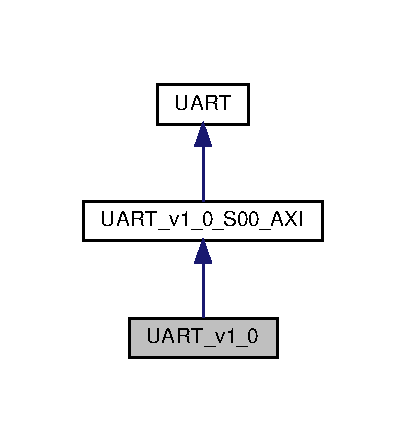
\includegraphics[width=195pt]{classUART__v1__0__inherit__graph}
\end{center}
\end{figure}


Collaboration diagram for U\+A\+R\+T\+\_\+v1\+\_\+0\+:
\nopagebreak
\begin{figure}[H]
\begin{center}
\leavevmode
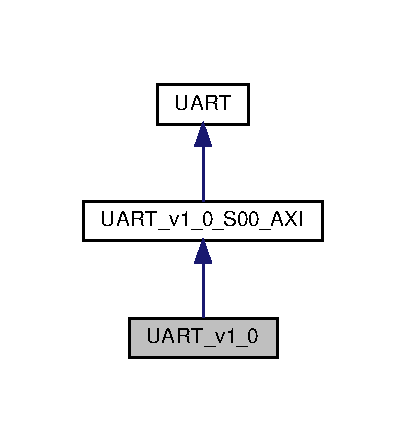
\includegraphics[width=195pt]{classUART__v1__0__coll__graph}
\end{center}
\end{figure}
\subsection*{Entities}
\begin{DoxyCompactItemize}
\item 
\hyperlink{classUART__v1__0_1_1arch__imp}{arch\+\_\+imp} architecture
\begin{DoxyCompactList}\small\item\em componente U\+A\+R\+T\+\_\+\+A\+X\+I\+\_\+\+S00  componente nel quale è incapsulato il componente \hyperlink{structUART}{U\+A\+RT} e la logica di gestione delle interruzioni. \end{DoxyCompactList}\end{DoxyCompactItemize}
\subsection*{Libraries}
 \begin{DoxyCompactItemize}
\item 
\mbox{\Hypertarget{classUART__v1__0_a0a6af6eef40212dbaf130d57ce711256}\label{classUART__v1__0_a0a6af6eef40212dbaf130d57ce711256}} 
\hyperlink{classUART__v1__0_a0a6af6eef40212dbaf130d57ce711256}{ieee} 
\begin{DoxyCompactList}\small\item\em Viene utilizzata la libreria I\+E\+EE. \end{DoxyCompactList}\end{DoxyCompactItemize}
\subsection*{Use Clauses}
 \begin{DoxyCompactItemize}
\item 
\mbox{\Hypertarget{classUART__v1__0_acd03516902501cd1c7296a98e22c6fcb}\label{classUART__v1__0_acd03516902501cd1c7296a98e22c6fcb}} 
\hyperlink{classUART__v1__0_acd03516902501cd1c7296a98e22c6fcb}{std\+\_\+logic\+\_\+1164}   
\begin{DoxyCompactList}\small\item\em Sono utilizzati i segnali della standard logic. \end{DoxyCompactList}\item 
\mbox{\Hypertarget{classUART__v1__0_a2edc34402b573437d5f25fa90ba4013e}\label{classUART__v1__0_a2edc34402b573437d5f25fa90ba4013e}} 
\hyperlink{classUART__v1__0_a2edc34402b573437d5f25fa90ba4013e}{numeric\+\_\+std}   
\begin{DoxyCompactList}\small\item\em Vengono utilizzate le funzioni numeriche. \end{DoxyCompactList}\end{DoxyCompactItemize}
\subsection*{Generics}
 \begin{DoxyCompactItemize}
\item 
\mbox{\Hypertarget{classUART__v1__0_af2979064a441fc814952a2a01b2e0bd3}\label{classUART__v1__0_af2979064a441fc814952a2a01b2e0bd3}} 
\hyperlink{classUART__v1__0_af2979064a441fc814952a2a01b2e0bd3}{baudrate} {\bfseries {\bfseries \textcolor{vhdlchar}{integer}\textcolor{vhdlchar}{ }\textcolor{vhdlchar}{ }\textcolor{vhdlchar}{\+:}\textcolor{vhdlchar}{=}\textcolor{vhdlchar}{ }\textcolor{vhdlchar}{ } \textcolor{vhdldigit}{9600} \textcolor{vhdlchar}{ }}}
\begin{DoxyCompactList}\small\item\em baudare trasmissione \end{DoxyCompactList}\item 
\mbox{\Hypertarget{classUART__v1__0_a378457a97325b4f40100f5b52b3dd886}\label{classUART__v1__0_a378457a97325b4f40100f5b52b3dd886}} 
\hyperlink{classUART__v1__0_a378457a97325b4f40100f5b52b3dd886}{clock\+\_\+freq} {\bfseries {\bfseries \textcolor{vhdlchar}{integer}\textcolor{vhdlchar}{ }\textcolor{vhdlchar}{ }\textcolor{vhdlchar}{\+:}\textcolor{vhdlchar}{=}\textcolor{vhdlchar}{ }\textcolor{vhdlchar}{ } \textcolor{vhdldigit}{50\+\_\+000\+\_\+000} \textcolor{vhdlchar}{ }}}
\begin{DoxyCompactList}\small\item\em frequenza clock ingresso \end{DoxyCompactList}\item 
\mbox{\Hypertarget{classUART__v1__0_afce7943994a4ddfa81f224225976a4c7}\label{classUART__v1__0_afce7943994a4ddfa81f224225976a4c7}} 
\hyperlink{classUART__v1__0_afce7943994a4ddfa81f224225976a4c7}{C\+\_\+\+S00\+\_\+\+A\+X\+I\+\_\+\+D\+A\+T\+A\+\_\+\+W\+I\+D\+TH} {\bfseries {\bfseries \textcolor{vhdlchar}{integer}\textcolor{vhdlchar}{ }\textcolor{vhdlchar}{ }\textcolor{vhdlchar}{\+:}\textcolor{vhdlchar}{=}\textcolor{vhdlchar}{ }\textcolor{vhdlchar}{ } \textcolor{vhdldigit}{32} \textcolor{vhdlchar}{ }}}
\item 
\mbox{\Hypertarget{classUART__v1__0_ab7787f274c76bb896ac98fdcfb570c65}\label{classUART__v1__0_ab7787f274c76bb896ac98fdcfb570c65}} 
\hyperlink{classUART__v1__0_ab7787f274c76bb896ac98fdcfb570c65}{C\+\_\+\+S00\+\_\+\+A\+X\+I\+\_\+\+A\+D\+D\+R\+\_\+\+W\+I\+D\+TH} {\bfseries {\bfseries \textcolor{vhdlchar}{integer}\textcolor{vhdlchar}{ }\textcolor{vhdlchar}{ }\textcolor{vhdlchar}{\+:}\textcolor{vhdlchar}{=}\textcolor{vhdlchar}{ }\textcolor{vhdlchar}{ } \textcolor{vhdldigit}{5} \textcolor{vhdlchar}{ }}}
\end{DoxyCompactItemize}
\subsection*{Ports}
 \begin{DoxyCompactItemize}
\item 
\mbox{\Hypertarget{classUART__v1__0_aa1eb566eeabe2a672e15ebb95aecc44f}\label{classUART__v1__0_aa1eb566eeabe2a672e15ebb95aecc44f}} 
\hyperlink{classUART__v1__0_aa1eb566eeabe2a672e15ebb95aecc44f}{tx}  {\bfseries {\bfseries \textcolor{vhdlchar}{out}\textcolor{vhdlchar}{ }}} {\bfseries \textcolor{vhdlchar}{std\+\_\+logic}\textcolor{vhdlchar}{ }} 
\begin{DoxyCompactList}\small\item\em linea uscita per la trasmissione \end{DoxyCompactList}\item 
\mbox{\Hypertarget{classUART__v1__0_a98ea5026beb91d6383a8a2aa2d69b32f}\label{classUART__v1__0_a98ea5026beb91d6383a8a2aa2d69b32f}} 
\hyperlink{classUART__v1__0_a98ea5026beb91d6383a8a2aa2d69b32f}{rx}  {\bfseries {\bfseries \textcolor{vhdlchar}{in}\textcolor{vhdlchar}{ }}} {\bfseries \textcolor{vhdlchar}{std\+\_\+logic}\textcolor{vhdlchar}{ }} 
\begin{DoxyCompactList}\small\item\em linea ingresso per la ricezione \end{DoxyCompactList}\item 
\mbox{\Hypertarget{classUART__v1__0_a5b78f3e3edfaf6e8ec79031b9e631e9d}\label{classUART__v1__0_a5b78f3e3edfaf6e8ec79031b9e631e9d}} 
\hyperlink{classUART__v1__0_a5b78f3e3edfaf6e8ec79031b9e631e9d}{interrupt}  {\bfseries {\bfseries \textcolor{vhdlchar}{out}\textcolor{vhdlchar}{ }}} {\bfseries \textcolor{vhdlchar}{std\+\_\+logic}\textcolor{vhdlchar}{ }} 
\begin{DoxyCompactList}\small\item\em segnale per richiede l\textquotesingle{}interrupt \end{DoxyCompactList}\item 
\mbox{\Hypertarget{classUART__v1__0_a037f9e3df8559bfd59db37bcba9cb7a8}\label{classUART__v1__0_a037f9e3df8559bfd59db37bcba9cb7a8}} 
\hyperlink{classUART__v1__0_a037f9e3df8559bfd59db37bcba9cb7a8}{s00\+\_\+axi\+\_\+aclk}  {\bfseries {\bfseries \textcolor{vhdlchar}{in}\textcolor{vhdlchar}{ }}} {\bfseries \textcolor{vhdlchar}{std\+\_\+logic}\textcolor{vhdlchar}{ }} 
\item 
\mbox{\Hypertarget{classUART__v1__0_a8249c106fbd80196dcad2666c9f0b3fc}\label{classUART__v1__0_a8249c106fbd80196dcad2666c9f0b3fc}} 
\hyperlink{classUART__v1__0_a8249c106fbd80196dcad2666c9f0b3fc}{s00\+\_\+axi\+\_\+aresetn}  {\bfseries {\bfseries \textcolor{vhdlchar}{in}\textcolor{vhdlchar}{ }}} {\bfseries \textcolor{vhdlchar}{std\+\_\+logic}\textcolor{vhdlchar}{ }} 
\item 
\mbox{\Hypertarget{classUART__v1__0_a9fe80d3cc7f862afb670536e4e05dbeb}\label{classUART__v1__0_a9fe80d3cc7f862afb670536e4e05dbeb}} 
\hyperlink{classUART__v1__0_a9fe80d3cc7f862afb670536e4e05dbeb}{s00\+\_\+axi\+\_\+awaddr}  {\bfseries {\bfseries \textcolor{vhdlchar}{in}\textcolor{vhdlchar}{ }}} {\bfseries \textcolor{vhdlchar}{std\+\_\+logic\+\_\+vector}\textcolor{vhdlchar}{ }\textcolor{vhdlchar}{(}\textcolor{vhdlchar}{ }\textcolor{vhdlchar}{ }\textcolor{vhdlchar}{ }\textcolor{vhdlchar}{ }\textcolor{vhdlchar}{C\+\_\+\+S00\+\_\+\+A\+X\+I\+\_\+\+A\+D\+D\+R\+\_\+\+W\+I\+D\+TH}\textcolor{vhdlchar}{-\/}\textcolor{vhdlchar}{ } \textcolor{vhdldigit}{1} \textcolor{vhdlchar}{ }\textcolor{vhdlchar}{downto}\textcolor{vhdlchar}{ }\textcolor{vhdlchar}{ } \textcolor{vhdldigit}{0} \textcolor{vhdlchar}{ }\textcolor{vhdlchar}{)}\textcolor{vhdlchar}{ }} 
\item 
\mbox{\Hypertarget{classUART__v1__0_a719659c1addef5432978cc949d9e10ed}\label{classUART__v1__0_a719659c1addef5432978cc949d9e10ed}} 
\hyperlink{classUART__v1__0_a719659c1addef5432978cc949d9e10ed}{s00\+\_\+axi\+\_\+awprot}  {\bfseries {\bfseries \textcolor{vhdlchar}{in}\textcolor{vhdlchar}{ }}} {\bfseries \textcolor{vhdlchar}{std\+\_\+logic\+\_\+vector}\textcolor{vhdlchar}{ }\textcolor{vhdlchar}{(}\textcolor{vhdlchar}{ }\textcolor{vhdlchar}{ } \textcolor{vhdldigit}{2} \textcolor{vhdlchar}{ }\textcolor{vhdlchar}{downto}\textcolor{vhdlchar}{ }\textcolor{vhdlchar}{ } \textcolor{vhdldigit}{0} \textcolor{vhdlchar}{ }\textcolor{vhdlchar}{)}\textcolor{vhdlchar}{ }} 
\item 
\mbox{\Hypertarget{classUART__v1__0_a45aa02a72ae1a8389346d47173c60ed0}\label{classUART__v1__0_a45aa02a72ae1a8389346d47173c60ed0}} 
\hyperlink{classUART__v1__0_a45aa02a72ae1a8389346d47173c60ed0}{s00\+\_\+axi\+\_\+awvalid}  {\bfseries {\bfseries \textcolor{vhdlchar}{in}\textcolor{vhdlchar}{ }}} {\bfseries \textcolor{vhdlchar}{std\+\_\+logic}\textcolor{vhdlchar}{ }} 
\item 
\mbox{\Hypertarget{classUART__v1__0_ad0a1f71502d91a45dbc6c365f85c6566}\label{classUART__v1__0_ad0a1f71502d91a45dbc6c365f85c6566}} 
\hyperlink{classUART__v1__0_ad0a1f71502d91a45dbc6c365f85c6566}{s00\+\_\+axi\+\_\+awready}  {\bfseries {\bfseries \textcolor{vhdlchar}{out}\textcolor{vhdlchar}{ }}} {\bfseries \textcolor{vhdlchar}{std\+\_\+logic}\textcolor{vhdlchar}{ }} 
\item 
\mbox{\Hypertarget{classUART__v1__0_ae2b15b55ee463fd9dd030ee29db6bb17}\label{classUART__v1__0_ae2b15b55ee463fd9dd030ee29db6bb17}} 
\hyperlink{classUART__v1__0_ae2b15b55ee463fd9dd030ee29db6bb17}{s00\+\_\+axi\+\_\+wdata}  {\bfseries {\bfseries \textcolor{vhdlchar}{in}\textcolor{vhdlchar}{ }}} {\bfseries \textcolor{vhdlchar}{std\+\_\+logic\+\_\+vector}\textcolor{vhdlchar}{ }\textcolor{vhdlchar}{(}\textcolor{vhdlchar}{ }\textcolor{vhdlchar}{ }\textcolor{vhdlchar}{ }\textcolor{vhdlchar}{ }\textcolor{vhdlchar}{C\+\_\+\+S00\+\_\+\+A\+X\+I\+\_\+\+D\+A\+T\+A\+\_\+\+W\+I\+D\+TH}\textcolor{vhdlchar}{-\/}\textcolor{vhdlchar}{ } \textcolor{vhdldigit}{1} \textcolor{vhdlchar}{ }\textcolor{vhdlchar}{downto}\textcolor{vhdlchar}{ }\textcolor{vhdlchar}{ } \textcolor{vhdldigit}{0} \textcolor{vhdlchar}{ }\textcolor{vhdlchar}{)}\textcolor{vhdlchar}{ }} 
\item 
\mbox{\Hypertarget{classUART__v1__0_a120924bc3fd5fd10ec0f96e19c3f4904}\label{classUART__v1__0_a120924bc3fd5fd10ec0f96e19c3f4904}} 
\hyperlink{classUART__v1__0_a120924bc3fd5fd10ec0f96e19c3f4904}{s00\+\_\+axi\+\_\+wstrb}  {\bfseries {\bfseries \textcolor{vhdlchar}{in}\textcolor{vhdlchar}{ }}} {\bfseries \textcolor{vhdlchar}{std\+\_\+logic\+\_\+vector}\textcolor{vhdlchar}{ }\textcolor{vhdlchar}{(}\textcolor{vhdlchar}{ }\textcolor{vhdlchar}{(}\textcolor{vhdlchar}{ }\textcolor{vhdlchar}{ }\textcolor{vhdlchar}{ }\textcolor{vhdlchar}{ }\textcolor{vhdlchar}{C\+\_\+\+S00\+\_\+\+A\+X\+I\+\_\+\+D\+A\+T\+A\+\_\+\+W\+I\+D\+TH}\textcolor{vhdlchar}{/}\textcolor{vhdlchar}{ } \textcolor{vhdldigit}{8} \textcolor{vhdlchar}{ }\textcolor{vhdlchar}{)}\textcolor{vhdlchar}{ }\textcolor{vhdlchar}{-\/}\textcolor{vhdlchar}{ } \textcolor{vhdldigit}{1} \textcolor{vhdlchar}{ }\textcolor{vhdlchar}{downto}\textcolor{vhdlchar}{ }\textcolor{vhdlchar}{ } \textcolor{vhdldigit}{0} \textcolor{vhdlchar}{ }\textcolor{vhdlchar}{)}\textcolor{vhdlchar}{ }} 
\item 
\mbox{\Hypertarget{classUART__v1__0_a24e90907193647007d2947353740114d}\label{classUART__v1__0_a24e90907193647007d2947353740114d}} 
\hyperlink{classUART__v1__0_a24e90907193647007d2947353740114d}{s00\+\_\+axi\+\_\+wvalid}  {\bfseries {\bfseries \textcolor{vhdlchar}{in}\textcolor{vhdlchar}{ }}} {\bfseries \textcolor{vhdlchar}{std\+\_\+logic}\textcolor{vhdlchar}{ }} 
\item 
\mbox{\Hypertarget{classUART__v1__0_a3fc60abc0cfbfa90003a83bffdd476c4}\label{classUART__v1__0_a3fc60abc0cfbfa90003a83bffdd476c4}} 
\hyperlink{classUART__v1__0_a3fc60abc0cfbfa90003a83bffdd476c4}{s00\+\_\+axi\+\_\+wready}  {\bfseries {\bfseries \textcolor{vhdlchar}{out}\textcolor{vhdlchar}{ }}} {\bfseries \textcolor{vhdlchar}{std\+\_\+logic}\textcolor{vhdlchar}{ }} 
\item 
\mbox{\Hypertarget{classUART__v1__0_af8799be946d3f5354263e7deb15f94f1}\label{classUART__v1__0_af8799be946d3f5354263e7deb15f94f1}} 
\hyperlink{classUART__v1__0_af8799be946d3f5354263e7deb15f94f1}{s00\+\_\+axi\+\_\+bresp}  {\bfseries {\bfseries \textcolor{vhdlchar}{out}\textcolor{vhdlchar}{ }}} {\bfseries \textcolor{vhdlchar}{std\+\_\+logic\+\_\+vector}\textcolor{vhdlchar}{ }\textcolor{vhdlchar}{(}\textcolor{vhdlchar}{ }\textcolor{vhdlchar}{ } \textcolor{vhdldigit}{1} \textcolor{vhdlchar}{ }\textcolor{vhdlchar}{downto}\textcolor{vhdlchar}{ }\textcolor{vhdlchar}{ } \textcolor{vhdldigit}{0} \textcolor{vhdlchar}{ }\textcolor{vhdlchar}{)}\textcolor{vhdlchar}{ }} 
\item 
\mbox{\Hypertarget{classUART__v1__0_a5110b7dd4fb9548a2aab88f50dbe1d5e}\label{classUART__v1__0_a5110b7dd4fb9548a2aab88f50dbe1d5e}} 
\hyperlink{classUART__v1__0_a5110b7dd4fb9548a2aab88f50dbe1d5e}{s00\+\_\+axi\+\_\+bvalid}  {\bfseries {\bfseries \textcolor{vhdlchar}{out}\textcolor{vhdlchar}{ }}} {\bfseries \textcolor{vhdlchar}{std\+\_\+logic}\textcolor{vhdlchar}{ }} 
\item 
\mbox{\Hypertarget{classUART__v1__0_a1ef2019b0613bc23d4829eeeb24eb98d}\label{classUART__v1__0_a1ef2019b0613bc23d4829eeeb24eb98d}} 
\hyperlink{classUART__v1__0_a1ef2019b0613bc23d4829eeeb24eb98d}{s00\+\_\+axi\+\_\+bready}  {\bfseries {\bfseries \textcolor{vhdlchar}{in}\textcolor{vhdlchar}{ }}} {\bfseries \textcolor{vhdlchar}{std\+\_\+logic}\textcolor{vhdlchar}{ }} 
\item 
\mbox{\Hypertarget{classUART__v1__0_af70a86336cd6505064e45b69f4623939}\label{classUART__v1__0_af70a86336cd6505064e45b69f4623939}} 
\hyperlink{classUART__v1__0_af70a86336cd6505064e45b69f4623939}{s00\+\_\+axi\+\_\+araddr}  {\bfseries {\bfseries \textcolor{vhdlchar}{in}\textcolor{vhdlchar}{ }}} {\bfseries \textcolor{vhdlchar}{std\+\_\+logic\+\_\+vector}\textcolor{vhdlchar}{ }\textcolor{vhdlchar}{(}\textcolor{vhdlchar}{ }\textcolor{vhdlchar}{ }\textcolor{vhdlchar}{ }\textcolor{vhdlchar}{ }\textcolor{vhdlchar}{C\+\_\+\+S00\+\_\+\+A\+X\+I\+\_\+\+A\+D\+D\+R\+\_\+\+W\+I\+D\+TH}\textcolor{vhdlchar}{-\/}\textcolor{vhdlchar}{ } \textcolor{vhdldigit}{1} \textcolor{vhdlchar}{ }\textcolor{vhdlchar}{downto}\textcolor{vhdlchar}{ }\textcolor{vhdlchar}{ } \textcolor{vhdldigit}{0} \textcolor{vhdlchar}{ }\textcolor{vhdlchar}{)}\textcolor{vhdlchar}{ }} 
\item 
\mbox{\Hypertarget{classUART__v1__0_adc648df07895bf808b8c721e1dc6811b}\label{classUART__v1__0_adc648df07895bf808b8c721e1dc6811b}} 
\hyperlink{classUART__v1__0_adc648df07895bf808b8c721e1dc6811b}{s00\+\_\+axi\+\_\+arprot}  {\bfseries {\bfseries \textcolor{vhdlchar}{in}\textcolor{vhdlchar}{ }}} {\bfseries \textcolor{vhdlchar}{std\+\_\+logic\+\_\+vector}\textcolor{vhdlchar}{ }\textcolor{vhdlchar}{(}\textcolor{vhdlchar}{ }\textcolor{vhdlchar}{ } \textcolor{vhdldigit}{2} \textcolor{vhdlchar}{ }\textcolor{vhdlchar}{downto}\textcolor{vhdlchar}{ }\textcolor{vhdlchar}{ } \textcolor{vhdldigit}{0} \textcolor{vhdlchar}{ }\textcolor{vhdlchar}{)}\textcolor{vhdlchar}{ }} 
\item 
\mbox{\Hypertarget{classUART__v1__0_a94b78b2ae3cd13860f15afbdfb199e44}\label{classUART__v1__0_a94b78b2ae3cd13860f15afbdfb199e44}} 
\hyperlink{classUART__v1__0_a94b78b2ae3cd13860f15afbdfb199e44}{s00\+\_\+axi\+\_\+arvalid}  {\bfseries {\bfseries \textcolor{vhdlchar}{in}\textcolor{vhdlchar}{ }}} {\bfseries \textcolor{vhdlchar}{std\+\_\+logic}\textcolor{vhdlchar}{ }} 
\item 
\mbox{\Hypertarget{classUART__v1__0_ad35bd95f3352ff8dbdaea55205a98e53}\label{classUART__v1__0_ad35bd95f3352ff8dbdaea55205a98e53}} 
\hyperlink{classUART__v1__0_ad35bd95f3352ff8dbdaea55205a98e53}{s00\+\_\+axi\+\_\+arready}  {\bfseries {\bfseries \textcolor{vhdlchar}{out}\textcolor{vhdlchar}{ }}} {\bfseries \textcolor{vhdlchar}{std\+\_\+logic}\textcolor{vhdlchar}{ }} 
\item 
\mbox{\Hypertarget{classUART__v1__0_ad2655fadb987e0487c428aca187b55d0}\label{classUART__v1__0_ad2655fadb987e0487c428aca187b55d0}} 
\hyperlink{classUART__v1__0_ad2655fadb987e0487c428aca187b55d0}{s00\+\_\+axi\+\_\+rdata}  {\bfseries {\bfseries \textcolor{vhdlchar}{out}\textcolor{vhdlchar}{ }}} {\bfseries \textcolor{vhdlchar}{std\+\_\+logic\+\_\+vector}\textcolor{vhdlchar}{ }\textcolor{vhdlchar}{(}\textcolor{vhdlchar}{ }\textcolor{vhdlchar}{ }\textcolor{vhdlchar}{ }\textcolor{vhdlchar}{ }\textcolor{vhdlchar}{C\+\_\+\+S00\+\_\+\+A\+X\+I\+\_\+\+D\+A\+T\+A\+\_\+\+W\+I\+D\+TH}\textcolor{vhdlchar}{-\/}\textcolor{vhdlchar}{ } \textcolor{vhdldigit}{1} \textcolor{vhdlchar}{ }\textcolor{vhdlchar}{downto}\textcolor{vhdlchar}{ }\textcolor{vhdlchar}{ } \textcolor{vhdldigit}{0} \textcolor{vhdlchar}{ }\textcolor{vhdlchar}{)}\textcolor{vhdlchar}{ }} 
\item 
\mbox{\Hypertarget{classUART__v1__0_a1acee955f50f71e5595a03c6ca301cf0}\label{classUART__v1__0_a1acee955f50f71e5595a03c6ca301cf0}} 
\hyperlink{classUART__v1__0_a1acee955f50f71e5595a03c6ca301cf0}{s00\+\_\+axi\+\_\+rresp}  {\bfseries {\bfseries \textcolor{vhdlchar}{out}\textcolor{vhdlchar}{ }}} {\bfseries \textcolor{vhdlchar}{std\+\_\+logic\+\_\+vector}\textcolor{vhdlchar}{ }\textcolor{vhdlchar}{(}\textcolor{vhdlchar}{ }\textcolor{vhdlchar}{ } \textcolor{vhdldigit}{1} \textcolor{vhdlchar}{ }\textcolor{vhdlchar}{downto}\textcolor{vhdlchar}{ }\textcolor{vhdlchar}{ } \textcolor{vhdldigit}{0} \textcolor{vhdlchar}{ }\textcolor{vhdlchar}{)}\textcolor{vhdlchar}{ }} 
\item 
\mbox{\Hypertarget{classUART__v1__0_af180911f7eb262e530e26865bc97aa0b}\label{classUART__v1__0_af180911f7eb262e530e26865bc97aa0b}} 
\hyperlink{classUART__v1__0_af180911f7eb262e530e26865bc97aa0b}{s00\+\_\+axi\+\_\+rvalid}  {\bfseries {\bfseries \textcolor{vhdlchar}{out}\textcolor{vhdlchar}{ }}} {\bfseries \textcolor{vhdlchar}{std\+\_\+logic}\textcolor{vhdlchar}{ }} 
\item 
\mbox{\Hypertarget{classUART__v1__0_a8b82eb165d7024f6c7b25646f6ebdd4d}\label{classUART__v1__0_a8b82eb165d7024f6c7b25646f6ebdd4d}} 
\hyperlink{classUART__v1__0_a8b82eb165d7024f6c7b25646f6ebdd4d}{s00\+\_\+axi\+\_\+rready}  {\bfseries {\bfseries \textcolor{vhdlchar}{in}\textcolor{vhdlchar}{ }}} {\bfseries \textcolor{vhdlchar}{std\+\_\+logic}\textcolor{vhdlchar}{ }} 
\end{DoxyCompactItemize}


The documentation for this class was generated from the following file\+:\begin{DoxyCompactItemize}
\item 
/media/saverio/\+O\+S/\+Users/\+Saverio/\+Desktop/\+S\+E/git/\+Andrea/\+F\+P\+G\+A/ip\+\_\+repo/\+U\+A\+R\+T\+\_\+1.\+0/hdl/\hyperlink{UART__v1__0_8vhd}{U\+A\+R\+T\+\_\+v1\+\_\+0.\+vhd}\end{DoxyCompactItemize}

\hypertarget{classUART__v1__0__S00__AXI}{}\section{U\+A\+R\+T\+\_\+v1\+\_\+0\+\_\+\+S00\+\_\+\+A\+XI Entity Reference}
\label{classUART__v1__0__S00__AXI}\index{U\+A\+R\+T\+\_\+v1\+\_\+0\+\_\+\+S00\+\_\+\+A\+XI@{U\+A\+R\+T\+\_\+v1\+\_\+0\+\_\+\+S00\+\_\+\+A\+XI}}


Inheritance diagram for U\+A\+R\+T\+\_\+v1\+\_\+0\+\_\+\+S00\+\_\+\+A\+XI\+:\nopagebreak
\begin{figure}[H]
\begin{center}
\leavevmode
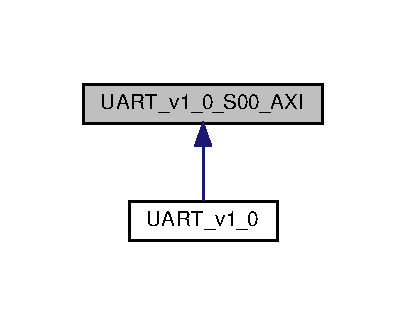
\includegraphics[width=195pt]{classUART__v1__0__S00__AXI__inherit__graph}
\end{center}
\end{figure}


Collaboration diagram for U\+A\+R\+T\+\_\+v1\+\_\+0\+\_\+\+S00\+\_\+\+A\+XI\+:\nopagebreak
\begin{figure}[H]
\begin{center}
\leavevmode
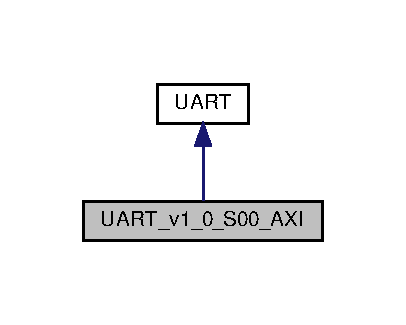
\includegraphics[width=195pt]{classUART__v1__0__S00__AXI__coll__graph}
\end{center}
\end{figure}
\subsection*{Entities}
\begin{DoxyCompactItemize}
\item 
\hyperlink{classUART__v1__0__S00__AXI_1_1arch__imp}{arch\+\_\+imp} architecture
\end{DoxyCompactItemize}
\subsection*{Libraries}
 \begin{DoxyCompactItemize}
\item 
\mbox{\Hypertarget{classUART__v1__0__S00__AXI_a0a6af6eef40212dbaf130d57ce711256}\label{classUART__v1__0__S00__AXI_a0a6af6eef40212dbaf130d57ce711256}} 
\hyperlink{classUART__v1__0__S00__AXI_a0a6af6eef40212dbaf130d57ce711256}{ieee} 
\begin{DoxyCompactList}\small\item\em Viene utilizzata la libreria I\+E\+EE. \end{DoxyCompactList}\end{DoxyCompactItemize}
\subsection*{Use Clauses}
 \begin{DoxyCompactItemize}
\item 
\mbox{\Hypertarget{classUART__v1__0__S00__AXI_acd03516902501cd1c7296a98e22c6fcb}\label{classUART__v1__0__S00__AXI_acd03516902501cd1c7296a98e22c6fcb}} 
\hyperlink{classUART__v1__0__S00__AXI_acd03516902501cd1c7296a98e22c6fcb}{std\+\_\+logic\+\_\+1164}   
\begin{DoxyCompactList}\small\item\em Sono utilizzati i segnali della standard logic. \end{DoxyCompactList}\item 
\mbox{\Hypertarget{classUART__v1__0__S00__AXI_a2edc34402b573437d5f25fa90ba4013e}\label{classUART__v1__0__S00__AXI_a2edc34402b573437d5f25fa90ba4013e}} 
\hyperlink{classUART__v1__0__S00__AXI_a2edc34402b573437d5f25fa90ba4013e}{numeric\+\_\+std}   
\begin{DoxyCompactList}\small\item\em Vengono utilizzate le funzioni numeriche. \end{DoxyCompactList}\item 
\mbox{\Hypertarget{classUART__v1__0__S00__AXI_acb2d98d781f19c8f5f4109576ec45502}\label{classUART__v1__0__S00__AXI_acb2d98d781f19c8f5f4109576ec45502}} 
\hyperlink{classUART__v1__0__S00__AXI_acb2d98d781f19c8f5f4109576ec45502}{std\+\_\+logic\+\_\+misc}   
\begin{DoxyCompactList}\small\item\em libreria necessaria per la funzione or\+\_\+reduce \end{DoxyCompactList}\end{DoxyCompactItemize}
\subsection*{Generics}
 \begin{DoxyCompactItemize}
\item 
\mbox{\Hypertarget{classUART__v1__0__S00__AXI_af2979064a441fc814952a2a01b2e0bd3}\label{classUART__v1__0__S00__AXI_af2979064a441fc814952a2a01b2e0bd3}} 
\hyperlink{classUART__v1__0__S00__AXI_af2979064a441fc814952a2a01b2e0bd3}{baudrate} {\bfseries {\bfseries \textcolor{vhdlchar}{integer}\textcolor{vhdlchar}{ }\textcolor{vhdlchar}{ }\textcolor{vhdlchar}{\+:}\textcolor{vhdlchar}{=}\textcolor{vhdlchar}{ }\textcolor{vhdlchar}{ } \textcolor{vhdldigit}{9600} \textcolor{vhdlchar}{ }}}
\item 
\mbox{\Hypertarget{classUART__v1__0__S00__AXI_a378457a97325b4f40100f5b52b3dd886}\label{classUART__v1__0__S00__AXI_a378457a97325b4f40100f5b52b3dd886}} 
\hyperlink{classUART__v1__0__S00__AXI_a378457a97325b4f40100f5b52b3dd886}{clock\+\_\+freq} {\bfseries {\bfseries \textcolor{vhdlchar}{integer}\textcolor{vhdlchar}{ }\textcolor{vhdlchar}{ }\textcolor{vhdlchar}{\+:}\textcolor{vhdlchar}{=}\textcolor{vhdlchar}{ }\textcolor{vhdlchar}{ } \textcolor{vhdldigit}{50\+\_\+000\+\_\+000} \textcolor{vhdlchar}{ }}}
\item 
\mbox{\Hypertarget{classUART__v1__0__S00__AXI_a0fad312acd1f302ce7de30c5658df0bd}\label{classUART__v1__0__S00__AXI_a0fad312acd1f302ce7de30c5658df0bd}} 
\hyperlink{classUART__v1__0__S00__AXI_a0fad312acd1f302ce7de30c5658df0bd}{C\+\_\+\+S\+\_\+\+A\+X\+I\+\_\+\+D\+A\+T\+A\+\_\+\+W\+I\+D\+TH} {\bfseries {\bfseries \textcolor{vhdlchar}{integer}\textcolor{vhdlchar}{ }\textcolor{vhdlchar}{ }\textcolor{vhdlchar}{\+:}\textcolor{vhdlchar}{=}\textcolor{vhdlchar}{ }\textcolor{vhdlchar}{ } \textcolor{vhdldigit}{32} \textcolor{vhdlchar}{ }}}
\item 
\mbox{\Hypertarget{classUART__v1__0__S00__AXI_a9abff2eaa069440f3b7d9e9937d5ee8e}\label{classUART__v1__0__S00__AXI_a9abff2eaa069440f3b7d9e9937d5ee8e}} 
\hyperlink{classUART__v1__0__S00__AXI_a9abff2eaa069440f3b7d9e9937d5ee8e}{C\+\_\+\+S\+\_\+\+A\+X\+I\+\_\+\+A\+D\+D\+R\+\_\+\+W\+I\+D\+TH} {\bfseries {\bfseries \textcolor{vhdlchar}{integer}\textcolor{vhdlchar}{ }\textcolor{vhdlchar}{ }\textcolor{vhdlchar}{\+:}\textcolor{vhdlchar}{=}\textcolor{vhdlchar}{ }\textcolor{vhdlchar}{ } \textcolor{vhdldigit}{5} \textcolor{vhdlchar}{ }}}
\end{DoxyCompactItemize}
\subsection*{Ports}
 \begin{DoxyCompactItemize}
\item 
\mbox{\Hypertarget{classUART__v1__0__S00__AXI_aa1eb566eeabe2a672e15ebb95aecc44f}\label{classUART__v1__0__S00__AXI_aa1eb566eeabe2a672e15ebb95aecc44f}} 
\hyperlink{classUART__v1__0__S00__AXI_aa1eb566eeabe2a672e15ebb95aecc44f}{tx}  {\bfseries {\bfseries \textcolor{vhdlchar}{out}\textcolor{vhdlchar}{ }}} {\bfseries \textcolor{vhdlchar}{std\+\_\+logic}\textcolor{vhdlchar}{ }} 
\item 
\mbox{\Hypertarget{classUART__v1__0__S00__AXI_a98ea5026beb91d6383a8a2aa2d69b32f}\label{classUART__v1__0__S00__AXI_a98ea5026beb91d6383a8a2aa2d69b32f}} 
\hyperlink{classUART__v1__0__S00__AXI_a98ea5026beb91d6383a8a2aa2d69b32f}{rx}  {\bfseries {\bfseries \textcolor{vhdlchar}{in}\textcolor{vhdlchar}{ }}} {\bfseries \textcolor{vhdlchar}{std\+\_\+logic}\textcolor{vhdlchar}{ }} 
\item 
\mbox{\Hypertarget{classUART__v1__0__S00__AXI_a5b78f3e3edfaf6e8ec79031b9e631e9d}\label{classUART__v1__0__S00__AXI_a5b78f3e3edfaf6e8ec79031b9e631e9d}} 
\hyperlink{classUART__v1__0__S00__AXI_a5b78f3e3edfaf6e8ec79031b9e631e9d}{interrupt}  {\bfseries {\bfseries \textcolor{vhdlchar}{out}\textcolor{vhdlchar}{ }}} {\bfseries \textcolor{vhdlchar}{std\+\_\+logic}\textcolor{vhdlchar}{ }} 
\item 
\mbox{\Hypertarget{classUART__v1__0__S00__AXI_a3f54d782a88290bdaa6baffd7cd84ab4}\label{classUART__v1__0__S00__AXI_a3f54d782a88290bdaa6baffd7cd84ab4}} 
\hyperlink{classUART__v1__0__S00__AXI_a3f54d782a88290bdaa6baffd7cd84ab4}{S\+\_\+\+A\+X\+I\+\_\+\+A\+C\+LK}  {\bfseries {\bfseries \textcolor{vhdlchar}{in}\textcolor{vhdlchar}{ }}} {\bfseries \textcolor{vhdlchar}{std\+\_\+logic}\textcolor{vhdlchar}{ }} 
\item 
\mbox{\Hypertarget{classUART__v1__0__S00__AXI_a089b396e17dee353ccc7d5389dda5532}\label{classUART__v1__0__S00__AXI_a089b396e17dee353ccc7d5389dda5532}} 
\hyperlink{classUART__v1__0__S00__AXI_a089b396e17dee353ccc7d5389dda5532}{S\+\_\+\+A\+X\+I\+\_\+\+A\+R\+E\+S\+E\+TN}  {\bfseries {\bfseries \textcolor{vhdlchar}{in}\textcolor{vhdlchar}{ }}} {\bfseries \textcolor{vhdlchar}{std\+\_\+logic}\textcolor{vhdlchar}{ }} 
\item 
\mbox{\Hypertarget{classUART__v1__0__S00__AXI_a61cc7b190ba9d540e56941330e4a0883}\label{classUART__v1__0__S00__AXI_a61cc7b190ba9d540e56941330e4a0883}} 
\hyperlink{classUART__v1__0__S00__AXI_a61cc7b190ba9d540e56941330e4a0883}{S\+\_\+\+A\+X\+I\+\_\+\+A\+W\+A\+D\+DR}  {\bfseries {\bfseries \textcolor{vhdlchar}{in}\textcolor{vhdlchar}{ }}} {\bfseries \textcolor{vhdlchar}{std\+\_\+logic\+\_\+vector}\textcolor{vhdlchar}{ }\textcolor{vhdlchar}{(}\textcolor{vhdlchar}{ }\textcolor{vhdlchar}{ }\textcolor{vhdlchar}{ }\textcolor{vhdlchar}{ }\textcolor{vhdlchar}{C\+\_\+\+S\+\_\+\+A\+X\+I\+\_\+\+A\+D\+D\+R\+\_\+\+W\+I\+D\+TH}\textcolor{vhdlchar}{-\/}\textcolor{vhdlchar}{ } \textcolor{vhdldigit}{1} \textcolor{vhdlchar}{ }\textcolor{vhdlchar}{downto}\textcolor{vhdlchar}{ }\textcolor{vhdlchar}{ } \textcolor{vhdldigit}{0} \textcolor{vhdlchar}{ }\textcolor{vhdlchar}{)}\textcolor{vhdlchar}{ }} 
\item 
\mbox{\Hypertarget{classUART__v1__0__S00__AXI_a459abcd98567ad24261377eed899593a}\label{classUART__v1__0__S00__AXI_a459abcd98567ad24261377eed899593a}} 
\hyperlink{classUART__v1__0__S00__AXI_a459abcd98567ad24261377eed899593a}{S\+\_\+\+A\+X\+I\+\_\+\+A\+W\+P\+R\+OT}  {\bfseries {\bfseries \textcolor{vhdlchar}{in}\textcolor{vhdlchar}{ }}} {\bfseries \textcolor{vhdlchar}{std\+\_\+logic\+\_\+vector}\textcolor{vhdlchar}{ }\textcolor{vhdlchar}{(}\textcolor{vhdlchar}{ }\textcolor{vhdlchar}{ } \textcolor{vhdldigit}{2} \textcolor{vhdlchar}{ }\textcolor{vhdlchar}{downto}\textcolor{vhdlchar}{ }\textcolor{vhdlchar}{ } \textcolor{vhdldigit}{0} \textcolor{vhdlchar}{ }\textcolor{vhdlchar}{)}\textcolor{vhdlchar}{ }} 
\item 
\mbox{\Hypertarget{classUART__v1__0__S00__AXI_af1f1cbf67bf647ba58353c261719a3a0}\label{classUART__v1__0__S00__AXI_af1f1cbf67bf647ba58353c261719a3a0}} 
\hyperlink{classUART__v1__0__S00__AXI_af1f1cbf67bf647ba58353c261719a3a0}{S\+\_\+\+A\+X\+I\+\_\+\+A\+W\+V\+A\+L\+ID}  {\bfseries {\bfseries \textcolor{vhdlchar}{in}\textcolor{vhdlchar}{ }}} {\bfseries \textcolor{vhdlchar}{std\+\_\+logic}\textcolor{vhdlchar}{ }} 
\item 
\mbox{\Hypertarget{classUART__v1__0__S00__AXI_ac04aab5cc834e762e893e061016921c6}\label{classUART__v1__0__S00__AXI_ac04aab5cc834e762e893e061016921c6}} 
\hyperlink{classUART__v1__0__S00__AXI_ac04aab5cc834e762e893e061016921c6}{S\+\_\+\+A\+X\+I\+\_\+\+A\+W\+R\+E\+A\+DY}  {\bfseries {\bfseries \textcolor{vhdlchar}{out}\textcolor{vhdlchar}{ }}} {\bfseries \textcolor{vhdlchar}{std\+\_\+logic}\textcolor{vhdlchar}{ }} 
\item 
\mbox{\Hypertarget{classUART__v1__0__S00__AXI_a292e5db13719faf3a8b3aab091773467}\label{classUART__v1__0__S00__AXI_a292e5db13719faf3a8b3aab091773467}} 
\hyperlink{classUART__v1__0__S00__AXI_a292e5db13719faf3a8b3aab091773467}{S\+\_\+\+A\+X\+I\+\_\+\+W\+D\+A\+TA}  {\bfseries {\bfseries \textcolor{vhdlchar}{in}\textcolor{vhdlchar}{ }}} {\bfseries \textcolor{vhdlchar}{std\+\_\+logic\+\_\+vector}\textcolor{vhdlchar}{ }\textcolor{vhdlchar}{(}\textcolor{vhdlchar}{ }\textcolor{vhdlchar}{ }\textcolor{vhdlchar}{ }\textcolor{vhdlchar}{ }\textcolor{vhdlchar}{C\+\_\+\+S\+\_\+\+A\+X\+I\+\_\+\+D\+A\+T\+A\+\_\+\+W\+I\+D\+TH}\textcolor{vhdlchar}{-\/}\textcolor{vhdlchar}{ } \textcolor{vhdldigit}{1} \textcolor{vhdlchar}{ }\textcolor{vhdlchar}{downto}\textcolor{vhdlchar}{ }\textcolor{vhdlchar}{ } \textcolor{vhdldigit}{0} \textcolor{vhdlchar}{ }\textcolor{vhdlchar}{)}\textcolor{vhdlchar}{ }} 
\item 
\mbox{\Hypertarget{classUART__v1__0__S00__AXI_accd8e04b79540b57ab15fee1cb6c04f5}\label{classUART__v1__0__S00__AXI_accd8e04b79540b57ab15fee1cb6c04f5}} 
\hyperlink{classUART__v1__0__S00__AXI_accd8e04b79540b57ab15fee1cb6c04f5}{S\+\_\+\+A\+X\+I\+\_\+\+W\+S\+T\+RB}  {\bfseries {\bfseries \textcolor{vhdlchar}{in}\textcolor{vhdlchar}{ }}} {\bfseries \textcolor{vhdlchar}{std\+\_\+logic\+\_\+vector}\textcolor{vhdlchar}{ }\textcolor{vhdlchar}{(}\textcolor{vhdlchar}{ }\textcolor{vhdlchar}{(}\textcolor{vhdlchar}{ }\textcolor{vhdlchar}{ }\textcolor{vhdlchar}{ }\textcolor{vhdlchar}{ }\textcolor{vhdlchar}{C\+\_\+\+S\+\_\+\+A\+X\+I\+\_\+\+D\+A\+T\+A\+\_\+\+W\+I\+D\+TH}\textcolor{vhdlchar}{/}\textcolor{vhdlchar}{ } \textcolor{vhdldigit}{8} \textcolor{vhdlchar}{ }\textcolor{vhdlchar}{)}\textcolor{vhdlchar}{ }\textcolor{vhdlchar}{-\/}\textcolor{vhdlchar}{ } \textcolor{vhdldigit}{1} \textcolor{vhdlchar}{ }\textcolor{vhdlchar}{downto}\textcolor{vhdlchar}{ }\textcolor{vhdlchar}{ } \textcolor{vhdldigit}{0} \textcolor{vhdlchar}{ }\textcolor{vhdlchar}{)}\textcolor{vhdlchar}{ }} 
\item 
\mbox{\Hypertarget{classUART__v1__0__S00__AXI_a60bd882e2de781af9a7c6c3d494225d5}\label{classUART__v1__0__S00__AXI_a60bd882e2de781af9a7c6c3d494225d5}} 
\hyperlink{classUART__v1__0__S00__AXI_a60bd882e2de781af9a7c6c3d494225d5}{S\+\_\+\+A\+X\+I\+\_\+\+W\+V\+A\+L\+ID}  {\bfseries {\bfseries \textcolor{vhdlchar}{in}\textcolor{vhdlchar}{ }}} {\bfseries \textcolor{vhdlchar}{std\+\_\+logic}\textcolor{vhdlchar}{ }} 
\item 
\mbox{\Hypertarget{classUART__v1__0__S00__AXI_ab84e4db7037141a360c2b59f45124f01}\label{classUART__v1__0__S00__AXI_ab84e4db7037141a360c2b59f45124f01}} 
\hyperlink{classUART__v1__0__S00__AXI_ab84e4db7037141a360c2b59f45124f01}{S\+\_\+\+A\+X\+I\+\_\+\+W\+R\+E\+A\+DY}  {\bfseries {\bfseries \textcolor{vhdlchar}{out}\textcolor{vhdlchar}{ }}} {\bfseries \textcolor{vhdlchar}{std\+\_\+logic}\textcolor{vhdlchar}{ }} 
\item 
\mbox{\Hypertarget{classUART__v1__0__S00__AXI_abca6c9777b38a5a6bc04886924bafcc8}\label{classUART__v1__0__S00__AXI_abca6c9777b38a5a6bc04886924bafcc8}} 
\hyperlink{classUART__v1__0__S00__AXI_abca6c9777b38a5a6bc04886924bafcc8}{S\+\_\+\+A\+X\+I\+\_\+\+B\+R\+E\+SP}  {\bfseries {\bfseries \textcolor{vhdlchar}{out}\textcolor{vhdlchar}{ }}} {\bfseries \textcolor{vhdlchar}{std\+\_\+logic\+\_\+vector}\textcolor{vhdlchar}{ }\textcolor{vhdlchar}{(}\textcolor{vhdlchar}{ }\textcolor{vhdlchar}{ } \textcolor{vhdldigit}{1} \textcolor{vhdlchar}{ }\textcolor{vhdlchar}{downto}\textcolor{vhdlchar}{ }\textcolor{vhdlchar}{ } \textcolor{vhdldigit}{0} \textcolor{vhdlchar}{ }\textcolor{vhdlchar}{)}\textcolor{vhdlchar}{ }} 
\item 
\mbox{\Hypertarget{classUART__v1__0__S00__AXI_a58f260d3ebaa69be91bb65ff9211823b}\label{classUART__v1__0__S00__AXI_a58f260d3ebaa69be91bb65ff9211823b}} 
\hyperlink{classUART__v1__0__S00__AXI_a58f260d3ebaa69be91bb65ff9211823b}{S\+\_\+\+A\+X\+I\+\_\+\+B\+V\+A\+L\+ID}  {\bfseries {\bfseries \textcolor{vhdlchar}{out}\textcolor{vhdlchar}{ }}} {\bfseries \textcolor{vhdlchar}{std\+\_\+logic}\textcolor{vhdlchar}{ }} 
\item 
\mbox{\Hypertarget{classUART__v1__0__S00__AXI_ac265989978a2be832d278f63fc0f06cb}\label{classUART__v1__0__S00__AXI_ac265989978a2be832d278f63fc0f06cb}} 
\hyperlink{classUART__v1__0__S00__AXI_ac265989978a2be832d278f63fc0f06cb}{S\+\_\+\+A\+X\+I\+\_\+\+B\+R\+E\+A\+DY}  {\bfseries {\bfseries \textcolor{vhdlchar}{in}\textcolor{vhdlchar}{ }}} {\bfseries \textcolor{vhdlchar}{std\+\_\+logic}\textcolor{vhdlchar}{ }} 
\item 
\mbox{\Hypertarget{classUART__v1__0__S00__AXI_a4d1dc8ecac269479747e5ac52c70ac45}\label{classUART__v1__0__S00__AXI_a4d1dc8ecac269479747e5ac52c70ac45}} 
\hyperlink{classUART__v1__0__S00__AXI_a4d1dc8ecac269479747e5ac52c70ac45}{S\+\_\+\+A\+X\+I\+\_\+\+A\+R\+A\+D\+DR}  {\bfseries {\bfseries \textcolor{vhdlchar}{in}\textcolor{vhdlchar}{ }}} {\bfseries \textcolor{vhdlchar}{std\+\_\+logic\+\_\+vector}\textcolor{vhdlchar}{ }\textcolor{vhdlchar}{(}\textcolor{vhdlchar}{ }\textcolor{vhdlchar}{ }\textcolor{vhdlchar}{ }\textcolor{vhdlchar}{ }\textcolor{vhdlchar}{C\+\_\+\+S\+\_\+\+A\+X\+I\+\_\+\+A\+D\+D\+R\+\_\+\+W\+I\+D\+TH}\textcolor{vhdlchar}{-\/}\textcolor{vhdlchar}{ } \textcolor{vhdldigit}{1} \textcolor{vhdlchar}{ }\textcolor{vhdlchar}{downto}\textcolor{vhdlchar}{ }\textcolor{vhdlchar}{ } \textcolor{vhdldigit}{0} \textcolor{vhdlchar}{ }\textcolor{vhdlchar}{)}\textcolor{vhdlchar}{ }} 
\item 
\mbox{\Hypertarget{classUART__v1__0__S00__AXI_a30a07c47d3c1182bbb7c904483bb374f}\label{classUART__v1__0__S00__AXI_a30a07c47d3c1182bbb7c904483bb374f}} 
\hyperlink{classUART__v1__0__S00__AXI_a30a07c47d3c1182bbb7c904483bb374f}{S\+\_\+\+A\+X\+I\+\_\+\+A\+R\+P\+R\+OT}  {\bfseries {\bfseries \textcolor{vhdlchar}{in}\textcolor{vhdlchar}{ }}} {\bfseries \textcolor{vhdlchar}{std\+\_\+logic\+\_\+vector}\textcolor{vhdlchar}{ }\textcolor{vhdlchar}{(}\textcolor{vhdlchar}{ }\textcolor{vhdlchar}{ } \textcolor{vhdldigit}{2} \textcolor{vhdlchar}{ }\textcolor{vhdlchar}{downto}\textcolor{vhdlchar}{ }\textcolor{vhdlchar}{ } \textcolor{vhdldigit}{0} \textcolor{vhdlchar}{ }\textcolor{vhdlchar}{)}\textcolor{vhdlchar}{ }} 
\item 
\mbox{\Hypertarget{classUART__v1__0__S00__AXI_a758f6340dd3340ee46deafbae18a47b2}\label{classUART__v1__0__S00__AXI_a758f6340dd3340ee46deafbae18a47b2}} 
\hyperlink{classUART__v1__0__S00__AXI_a758f6340dd3340ee46deafbae18a47b2}{S\+\_\+\+A\+X\+I\+\_\+\+A\+R\+V\+A\+L\+ID}  {\bfseries {\bfseries \textcolor{vhdlchar}{in}\textcolor{vhdlchar}{ }}} {\bfseries \textcolor{vhdlchar}{std\+\_\+logic}\textcolor{vhdlchar}{ }} 
\item 
\mbox{\Hypertarget{classUART__v1__0__S00__AXI_ade4e78e9c32af26578fc5c74ca3197e8}\label{classUART__v1__0__S00__AXI_ade4e78e9c32af26578fc5c74ca3197e8}} 
\hyperlink{classUART__v1__0__S00__AXI_ade4e78e9c32af26578fc5c74ca3197e8}{S\+\_\+\+A\+X\+I\+\_\+\+A\+R\+R\+E\+A\+DY}  {\bfseries {\bfseries \textcolor{vhdlchar}{out}\textcolor{vhdlchar}{ }}} {\bfseries \textcolor{vhdlchar}{std\+\_\+logic}\textcolor{vhdlchar}{ }} 
\item 
\mbox{\Hypertarget{classUART__v1__0__S00__AXI_a194c6eff7c88405e7934dbc2425ee4ab}\label{classUART__v1__0__S00__AXI_a194c6eff7c88405e7934dbc2425ee4ab}} 
\hyperlink{classUART__v1__0__S00__AXI_a194c6eff7c88405e7934dbc2425ee4ab}{S\+\_\+\+A\+X\+I\+\_\+\+R\+D\+A\+TA}  {\bfseries {\bfseries \textcolor{vhdlchar}{out}\textcolor{vhdlchar}{ }}} {\bfseries \textcolor{vhdlchar}{std\+\_\+logic\+\_\+vector}\textcolor{vhdlchar}{ }\textcolor{vhdlchar}{(}\textcolor{vhdlchar}{ }\textcolor{vhdlchar}{ }\textcolor{vhdlchar}{ }\textcolor{vhdlchar}{ }\textcolor{vhdlchar}{C\+\_\+\+S\+\_\+\+A\+X\+I\+\_\+\+D\+A\+T\+A\+\_\+\+W\+I\+D\+TH}\textcolor{vhdlchar}{-\/}\textcolor{vhdlchar}{ } \textcolor{vhdldigit}{1} \textcolor{vhdlchar}{ }\textcolor{vhdlchar}{downto}\textcolor{vhdlchar}{ }\textcolor{vhdlchar}{ } \textcolor{vhdldigit}{0} \textcolor{vhdlchar}{ }\textcolor{vhdlchar}{)}\textcolor{vhdlchar}{ }} 
\item 
\mbox{\Hypertarget{classUART__v1__0__S00__AXI_a67ba85504b4c51fb0eb00d18fd70ad92}\label{classUART__v1__0__S00__AXI_a67ba85504b4c51fb0eb00d18fd70ad92}} 
\hyperlink{classUART__v1__0__S00__AXI_a67ba85504b4c51fb0eb00d18fd70ad92}{S\+\_\+\+A\+X\+I\+\_\+\+R\+R\+E\+SP}  {\bfseries {\bfseries \textcolor{vhdlchar}{out}\textcolor{vhdlchar}{ }}} {\bfseries \textcolor{vhdlchar}{std\+\_\+logic\+\_\+vector}\textcolor{vhdlchar}{ }\textcolor{vhdlchar}{(}\textcolor{vhdlchar}{ }\textcolor{vhdlchar}{ } \textcolor{vhdldigit}{1} \textcolor{vhdlchar}{ }\textcolor{vhdlchar}{downto}\textcolor{vhdlchar}{ }\textcolor{vhdlchar}{ } \textcolor{vhdldigit}{0} \textcolor{vhdlchar}{ }\textcolor{vhdlchar}{)}\textcolor{vhdlchar}{ }} 
\item 
\mbox{\Hypertarget{classUART__v1__0__S00__AXI_a31f4e92d27c2c2005ee5f368a8249604}\label{classUART__v1__0__S00__AXI_a31f4e92d27c2c2005ee5f368a8249604}} 
\hyperlink{classUART__v1__0__S00__AXI_a31f4e92d27c2c2005ee5f368a8249604}{S\+\_\+\+A\+X\+I\+\_\+\+R\+V\+A\+L\+ID}  {\bfseries {\bfseries \textcolor{vhdlchar}{out}\textcolor{vhdlchar}{ }}} {\bfseries \textcolor{vhdlchar}{std\+\_\+logic}\textcolor{vhdlchar}{ }} 
\item 
\mbox{\Hypertarget{classUART__v1__0__S00__AXI_a5850bf8f42acdf01938057507dc703b7}\label{classUART__v1__0__S00__AXI_a5850bf8f42acdf01938057507dc703b7}} 
\hyperlink{classUART__v1__0__S00__AXI_a5850bf8f42acdf01938057507dc703b7}{S\+\_\+\+A\+X\+I\+\_\+\+R\+R\+E\+A\+DY}  {\bfseries {\bfseries \textcolor{vhdlchar}{in}\textcolor{vhdlchar}{ }}} {\bfseries \textcolor{vhdlchar}{std\+\_\+logic}\textcolor{vhdlchar}{ }} 
\end{DoxyCompactItemize}


The documentation for this class was generated from the following file\+:\begin{DoxyCompactItemize}
\item 
/media/saverio/\+O\+S/\+Users/\+Saverio/\+Desktop/\+S\+E/git/codici\+\_\+da\+\_\+mandare/\+F\+P\+G\+A/\+U\+A\+R\+T/\+Hardware/\+U\+A\+R\+T\+\_\+1.\+0/hdl/\hyperlink{UART__v1__0__S00__AXI_8vhd}{U\+A\+R\+T\+\_\+v1\+\_\+0\+\_\+\+S00\+\_\+\+A\+X\+I.\+vhd}\end{DoxyCompactItemize}

\chapter{File Documentation}
\hypertarget{UART__v1__0_8vhd}{}\section{/media/saverio/\+O\+S/\+Users/\+Saverio/\+Desktop/\+S\+E/git/\+Andrea/\+F\+P\+G\+A/ip\+\_\+repo/\+U\+A\+R\+T\+\_\+1.0/hdl/\+U\+A\+R\+T\+\_\+v1\+\_\+0.vhd File Reference}
\label{UART__v1__0_8vhd}\index{/media/saverio/\+O\+S/\+Users/\+Saverio/\+Desktop/\+S\+E/git/\+Andrea/\+F\+P\+G\+A/ip\+\_\+repo/\+U\+A\+R\+T\+\_\+1.\+0/hdl/\+U\+A\+R\+T\+\_\+v1\+\_\+0.\+vhd@{/media/saverio/\+O\+S/\+Users/\+Saverio/\+Desktop/\+S\+E/git/\+Andrea/\+F\+P\+G\+A/ip\+\_\+repo/\+U\+A\+R\+T\+\_\+1.\+0/hdl/\+U\+A\+R\+T\+\_\+v1\+\_\+0.\+vhd}}


U\+A\+RT A\+XI I\+P\+C\+O\+RE with interrupt.  


\subsection*{Entities}
\begin{DoxyCompactItemize}
\item 
\hyperlink{classUART__v1__0}{U\+A\+R\+T\+\_\+v1\+\_\+0} entity
\item 
\hyperlink{classUART__v1__0_1_1arch__imp}{arch\+\_\+imp} architecture
\begin{DoxyCompactList}\small\item\em componente U\+A\+R\+T\+\_\+\+A\+X\+I\+\_\+\+S00  componente nel quale è incapsulato il componente U\+A\+RT e la logica di gestione delle interruzioni. \end{DoxyCompactList}\end{DoxyCompactItemize}


\subsection{Detailed Description}
U\+A\+RT A\+XI I\+P\+C\+O\+RE with interrupt. 


\hypertarget{UART__v1__0__S00__AXI_8vhd}{}\section{/media/saverio/\+O\+S/\+Users/\+Saverio/\+Desktop/\+S\+E/git/\+Andrea/\+F\+P\+G\+A/ip\+\_\+repo/\+U\+A\+R\+T\+\_\+1.0/hdl/\+U\+A\+R\+T\+\_\+v1\+\_\+0\+\_\+\+S00\+\_\+\+A\+XI.vhd File Reference}
\label{UART__v1__0__S00__AXI_8vhd}\index{/media/saverio/\+O\+S/\+Users/\+Saverio/\+Desktop/\+S\+E/git/\+Andrea/\+F\+P\+G\+A/ip\+\_\+repo/\+U\+A\+R\+T\+\_\+1.\+0/hdl/\+U\+A\+R\+T\+\_\+v1\+\_\+0\+\_\+\+S00\+\_\+\+A\+X\+I.\+vhd@{/media/saverio/\+O\+S/\+Users/\+Saverio/\+Desktop/\+S\+E/git/\+Andrea/\+F\+P\+G\+A/ip\+\_\+repo/\+U\+A\+R\+T\+\_\+1.\+0/hdl/\+U\+A\+R\+T\+\_\+v1\+\_\+0\+\_\+\+S00\+\_\+\+A\+X\+I.\+vhd}}


\hyperlink{structUART}{U\+A\+RT} A\+XI I\+P\+C\+O\+RE with interrupt.  


\subsection*{Entities}
\begin{DoxyCompactItemize}
\item 
\hyperlink{classUART__v1__0__S00__AXI}{U\+A\+R\+T\+\_\+v1\+\_\+0\+\_\+\+S00\+\_\+\+A\+XI} entity
\item 
\hyperlink{classUART__v1__0__S00__AXI_1_1arch__imp}{arch\+\_\+imp} architecture
\end{DoxyCompactItemize}


\subsection{Detailed Description}
\hyperlink{structUART}{U\+A\+RT} A\+XI I\+P\+C\+O\+RE with interrupt. 


\hypertarget{GPIO_8c}{}\section{/media/saverio/\+O\+S/\+Users/\+Saverio/\+Desktop/\+S\+E/git/codici\+\_\+da\+\_\+mandare/\+F\+P\+G\+A/\+G\+P\+I\+O/\+Driver/\+Kernel\+\_\+\+Mode/\+G\+P\+IO.c File Reference}
\label{GPIO_8c}\index{/media/saverio/\+O\+S/\+Users/\+Saverio/\+Desktop/\+S\+E/git/codici\+\_\+da\+\_\+mandare/\+F\+P\+G\+A/\+G\+P\+I\+O/\+Driver/\+Kernel\+\_\+\+Mode/\+G\+P\+I\+O.\+c@{/media/saverio/\+O\+S/\+Users/\+Saverio/\+Desktop/\+S\+E/git/codici\+\_\+da\+\_\+mandare/\+F\+P\+G\+A/\+G\+P\+I\+O/\+Driver/\+Kernel\+\_\+\+Mode/\+G\+P\+I\+O.\+c}}


Funzioni utilizzate per interagire con la singola entità \hyperlink{structGPIO}{G\+P\+IO} permette la gestione dell\textquotesingle{} interrupt.  




\subsection{Detailed Description}
Funzioni utilizzate per interagire con la singola entità \hyperlink{structGPIO}{G\+P\+IO} permette la gestione dell\textquotesingle{} interrupt. 



\subsection{Function Documentation}
\mbox{\Hypertarget{GPIO_8c_a35e453e72ddf756e45ee2d312eb760ab}\label{GPIO_8c_a35e453e72ddf756e45ee2d312eb760ab}} 
\index{G\+P\+I\+O.\+c@{G\+P\+I\+O.\+c}!G\+P\+I\+O\+\_\+\+Destroy@{G\+P\+I\+O\+\_\+\+Destroy}}
\index{G\+P\+I\+O\+\_\+\+Destroy@{G\+P\+I\+O\+\_\+\+Destroy}!G\+P\+I\+O.\+c@{G\+P\+I\+O.\+c}}
\subsubsection{\texorpdfstring{G\+P\+I\+O\+\_\+\+Destroy()}{GPIO\_Destroy()}}
{\footnotesize\ttfamily void G\+P\+I\+O\+\_\+\+Destroy (\begin{DoxyParamCaption}\item[{\hyperlink{structGPIO}{G\+P\+IO}$\ast$}]{device }\end{DoxyParamCaption})}



Rimuove un device \hyperlink{structGPIO}{G\+P\+IO} con le relative strutture kernel allocate per il suo funzionamento. 


\begin{DoxyParams}{Parameters}
{\em device} & puntatore a struttura \hyperlink{structGPIO}{G\+P\+IO} che indica l\textquotesingle{}istanza \hyperlink{structGPIO}{G\+P\+IO} da rimuovere \\
\hline
\end{DoxyParams}
\mbox{\Hypertarget{GPIO_8c_a88017c9a3bf24e68865541255a3cf065}\label{GPIO_8c_a88017c9a3bf24e68865541255a3cf065}} 
\index{G\+P\+I\+O.\+c@{G\+P\+I\+O.\+c}!G\+P\+I\+O\+\_\+\+Get\+Device\+Address@{G\+P\+I\+O\+\_\+\+Get\+Device\+Address}}
\index{G\+P\+I\+O\+\_\+\+Get\+Device\+Address@{G\+P\+I\+O\+\_\+\+Get\+Device\+Address}!G\+P\+I\+O.\+c@{G\+P\+I\+O.\+c}}
\subsubsection{\texorpdfstring{G\+P\+I\+O\+\_\+\+Get\+Device\+Address()}{GPIO\_GetDeviceAddress()}}
{\footnotesize\ttfamily void$\ast$ G\+P\+I\+O\+\_\+\+Get\+Device\+Address (\begin{DoxyParamCaption}\item[{\hyperlink{structGPIO}{G\+P\+IO}$\ast$}]{device }\end{DoxyParamCaption})}



Restituisce l\textquotesingle{}indirizzo virtuale di memoria cui è mappato un device. 


\begin{DoxyParams}{Parameters}
{\em device} & puntatore a struttura \hyperlink{structGPIO}{G\+P\+IO}, che si riferisce al device su cui operare \\
\hline
\end{DoxyParams}
\mbox{\Hypertarget{GPIO_8c_abfd5d2d0153f5cbea672c14fb78f500b}\label{GPIO_8c_abfd5d2d0153f5cbea672c14fb78f500b}} 
\index{G\+P\+I\+O.\+c@{G\+P\+I\+O.\+c}!G\+P\+I\+O\+\_\+\+Get\+Poll\+Mask@{G\+P\+I\+O\+\_\+\+Get\+Poll\+Mask}}
\index{G\+P\+I\+O\+\_\+\+Get\+Poll\+Mask@{G\+P\+I\+O\+\_\+\+Get\+Poll\+Mask}!G\+P\+I\+O.\+c@{G\+P\+I\+O.\+c}}
\subsubsection{\texorpdfstring{G\+P\+I\+O\+\_\+\+Get\+Poll\+Mask()}{GPIO\_GetPollMask()}}
{\footnotesize\ttfamily unsigned G\+P\+I\+O\+\_\+\+Get\+Poll\+Mask (\begin{DoxyParamCaption}\item[{\hyperlink{structGPIO}{G\+P\+IO} $\ast$}]{device,  }\item[{struct file $\ast$}]{file\+\_\+ptr,  }\item[{struct poll\+\_\+table\+\_\+struct $\ast$}]{wait }\end{DoxyParamCaption})}



Verifica che le operazioni di lettura risultino non-\/bloccanti. 


\begin{DoxyParams}{Parameters}
{\em device} & puntatore a struttura \hyperlink{structGPIO}{G\+P\+IO}, che si riferisce al device su cui operare \\
\hline
{\em file} & puntatore al descrittore file del device \\
\hline
{\em wait} & puntatore alla struttura poll\+\_\+table\\
\hline
\end{DoxyParams}
\begin{DoxyReturn}{Returns}
maschera di bit che indica se sia possibile effettuare operazioni di lettura non bloccanti.
\end{DoxyReturn}
Back-\/end di tre diverse sys-\/calls\+: poll, epoll e select, \mbox{\Hypertarget{GPIO_8c_a9acce2a93067430307df45f0cc8aa02a}\label{GPIO_8c_a9acce2a93067430307df45f0cc8aa02a}} 
\index{G\+P\+I\+O.\+c@{G\+P\+I\+O.\+c}!G\+P\+I\+O\+\_\+\+Global\+Interrupt\+Disable@{G\+P\+I\+O\+\_\+\+Global\+Interrupt\+Disable}}
\index{G\+P\+I\+O\+\_\+\+Global\+Interrupt\+Disable@{G\+P\+I\+O\+\_\+\+Global\+Interrupt\+Disable}!G\+P\+I\+O.\+c@{G\+P\+I\+O.\+c}}
\subsubsection{\texorpdfstring{G\+P\+I\+O\+\_\+\+Global\+Interrupt\+Disable()}{GPIO\_GlobalInterruptDisable()}}
{\footnotesize\ttfamily void G\+P\+I\+O\+\_\+\+Global\+Interrupt\+Disable (\begin{DoxyParamCaption}\item[{\hyperlink{structGPIO}{G\+P\+IO}$\ast$}]{device }\end{DoxyParamCaption})}



Disabilitazione interrupt globali;. 


\begin{DoxyParams}{Parameters}
{\em device} & puntatore a struttura \hyperlink{structGPIO}{G\+P\+IO}, che si riferisce al device su cui operare \\
\hline
\end{DoxyParams}
\mbox{\Hypertarget{GPIO_8c_ace8fd580466277115b8b7d913d050823}\label{GPIO_8c_ace8fd580466277115b8b7d913d050823}} 
\index{G\+P\+I\+O.\+c@{G\+P\+I\+O.\+c}!G\+P\+I\+O\+\_\+\+Global\+Interrupt\+Enable@{G\+P\+I\+O\+\_\+\+Global\+Interrupt\+Enable}}
\index{G\+P\+I\+O\+\_\+\+Global\+Interrupt\+Enable@{G\+P\+I\+O\+\_\+\+Global\+Interrupt\+Enable}!G\+P\+I\+O.\+c@{G\+P\+I\+O.\+c}}
\subsubsection{\texorpdfstring{G\+P\+I\+O\+\_\+\+Global\+Interrupt\+Enable()}{GPIO\_GlobalInterruptEnable()}}
{\footnotesize\ttfamily void G\+P\+I\+O\+\_\+\+Global\+Interrupt\+Enable (\begin{DoxyParamCaption}\item[{\hyperlink{structGPIO}{G\+P\+IO}$\ast$}]{device }\end{DoxyParamCaption})}



Abilitazione interrupt globali;. 


\begin{DoxyParams}{Parameters}
{\em device} & puntatore a struttura \hyperlink{structGPIO}{G\+P\+IO}, che si riferisce al device su cui operare \\
\hline
\end{DoxyParams}
\mbox{\Hypertarget{GPIO_8c_ad1d3c415a8f65c105fb7d4baf4e29e5c}\label{GPIO_8c_ad1d3c415a8f65c105fb7d4baf4e29e5c}} 
\index{G\+P\+I\+O.\+c@{G\+P\+I\+O.\+c}!G\+P\+I\+O\+\_\+\+Init@{G\+P\+I\+O\+\_\+\+Init}}
\index{G\+P\+I\+O\+\_\+\+Init@{G\+P\+I\+O\+\_\+\+Init}!G\+P\+I\+O.\+c@{G\+P\+I\+O.\+c}}
\subsubsection{\texorpdfstring{G\+P\+I\+O\+\_\+\+Init()}{GPIO\_Init()}}
{\footnotesize\ttfamily int G\+P\+I\+O\+\_\+\+Init (\begin{DoxyParamCaption}\item[{\hyperlink{structGPIO}{G\+P\+IO}$\ast$}]{G\+P\+I\+O\+\_\+device,  }\item[{struct module $\ast$}]{owner,  }\item[{struct platform\+\_\+device $\ast$}]{pdev,  }\item[{struct class$\ast$}]{class,  }\item[{const char$\ast$}]{driver\+\_\+name,  }\item[{const char$\ast$}]{device\+\_\+name,  }\item[{uint32\+\_\+t}]{serial,  }\item[{struct file\+\_\+operations $\ast$}]{f\+\_\+ops,  }\item[{irq\+\_\+handler\+\_\+t}]{irq\+\_\+handler,  }\item[{uint32\+\_\+t}]{irq\+\_\+mask }\end{DoxyParamCaption})}



Inizializza una struttura \hyperlink{structGPIO}{G\+P\+IO} per il corrispondente device. 


\begin{DoxyParams}{Parameters}
{\em G\+P\+I\+O\+\_\+device} & puntatore a struttura \hyperlink{structGPIO}{G\+P\+IO}, corrispondente al device su cui operare \\
\hline
{\em owner} & puntatore a struttura struct module, proprietario del device (T\+H\+I\+S\+\_\+\+M\+O\+D\+U\+LE) \\
\hline
{\em pdev} & puntatore a struct platform\+\_\+device \\
\hline
{\em driver\+\_\+name} & nome del driver \\
\hline
{\em device\+\_\+name} & nome del device \\
\hline
{\em serial} & numero seriale del device \\
\hline
{\em f\+\_\+ops} & puntatore a struttura struct file\+\_\+operations, specifica le funzioni che agiscono sul device \\
\hline
{\em irq\+\_\+handler} & puntatore irq\+\_\+handler\+\_\+t alla funzione che gestisce gli interrupt generati dal device \\
\hline
{\em irq\+\_\+mask} & maschera delle interruzioni attive del device\\
\hline
\end{DoxyParams}

\begin{DoxyRetVals}{Return values}
{\em 0} & se non si è verificato nessun errore \\
\hline
\end{DoxyRetVals}
Inizializzazione della wait-\/queue per la system-\/call read() e poll()

Inizializzazione degli spinlock

Abilitazione degli interrupt del device \mbox{\Hypertarget{GPIO_8c_a0c89651b9f8711b02a3584f1968fac3b}\label{GPIO_8c_a0c89651b9f8711b02a3584f1968fac3b}} 
\index{G\+P\+I\+O.\+c@{G\+P\+I\+O.\+c}!G\+P\+I\+O\+\_\+\+Pending\+Pin\+Interrupt@{G\+P\+I\+O\+\_\+\+Pending\+Pin\+Interrupt}}
\index{G\+P\+I\+O\+\_\+\+Pending\+Pin\+Interrupt@{G\+P\+I\+O\+\_\+\+Pending\+Pin\+Interrupt}!G\+P\+I\+O.\+c@{G\+P\+I\+O.\+c}}
\subsubsection{\texorpdfstring{G\+P\+I\+O\+\_\+\+Pending\+Pin\+Interrupt()}{GPIO\_PendingPinInterrupt()}}
{\footnotesize\ttfamily unsigned G\+P\+I\+O\+\_\+\+Pending\+Pin\+Interrupt (\begin{DoxyParamCaption}\item[{\hyperlink{structGPIO}{G\+P\+IO}$\ast$}]{device }\end{DoxyParamCaption})}



Fornisce una maschera che indica quali interrupt non sono ancora stati serviti e che quindi risultano pending. 


\begin{DoxyParams}{Parameters}
{\em device} & puntatore a struttura \hyperlink{structGPIO}{G\+P\+IO}, che si riferisce al device su cui operare\\
\hline
\end{DoxyParams}
\begin{DoxyReturn}{Returns}
maschera riportante i pin per i quali gli interrupt non sono stati ancora serviti 
\end{DoxyReturn}
\mbox{\Hypertarget{GPIO_8c_af8147f170ccf8ee218d04b6aca631ba3}\label{GPIO_8c_af8147f170ccf8ee218d04b6aca631ba3}} 
\index{G\+P\+I\+O.\+c@{G\+P\+I\+O.\+c}!G\+P\+I\+O\+\_\+\+Pin\+Interrupt\+Ack@{G\+P\+I\+O\+\_\+\+Pin\+Interrupt\+Ack}}
\index{G\+P\+I\+O\+\_\+\+Pin\+Interrupt\+Ack@{G\+P\+I\+O\+\_\+\+Pin\+Interrupt\+Ack}!G\+P\+I\+O.\+c@{G\+P\+I\+O.\+c}}
\subsubsection{\texorpdfstring{G\+P\+I\+O\+\_\+\+Pin\+Interrupt\+Ack()}{GPIO\_PinInterruptAck()}}
{\footnotesize\ttfamily void G\+P\+I\+O\+\_\+\+Pin\+Interrupt\+Ack (\begin{DoxyParamCaption}\item[{\hyperlink{structGPIO}{G\+P\+IO}$\ast$}]{device,  }\item[{unsigned}]{mask }\end{DoxyParamCaption})}



Invia al device notifica di servizio di un interrupt;. 


\begin{DoxyParams}{Parameters}
{\em device} & puntatore a struttura \hyperlink{structGPIO}{G\+P\+IO}, che si riferisce al device su cui operare\\
\hline
{\em mask} & maschera di selezione degli interrupt da notificare \\
\hline
\end{DoxyParams}
\mbox{\Hypertarget{GPIO_8c_aa6651afb078323181b89b424bdae1b32}\label{GPIO_8c_aa6651afb078323181b89b424bdae1b32}} 
\index{G\+P\+I\+O.\+c@{G\+P\+I\+O.\+c}!G\+P\+I\+O\+\_\+\+Pin\+Interrupt\+Disable@{G\+P\+I\+O\+\_\+\+Pin\+Interrupt\+Disable}}
\index{G\+P\+I\+O\+\_\+\+Pin\+Interrupt\+Disable@{G\+P\+I\+O\+\_\+\+Pin\+Interrupt\+Disable}!G\+P\+I\+O.\+c@{G\+P\+I\+O.\+c}}
\subsubsection{\texorpdfstring{G\+P\+I\+O\+\_\+\+Pin\+Interrupt\+Disable()}{GPIO\_PinInterruptDisable()}}
{\footnotesize\ttfamily void G\+P\+I\+O\+\_\+\+Pin\+Interrupt\+Disable (\begin{DoxyParamCaption}\item[{\hyperlink{structGPIO}{G\+P\+IO}$\ast$}]{device,  }\item[{unsigned}]{mask }\end{DoxyParamCaption})}



Disabilitazione interrupt per i singoli pin del device. 


\begin{DoxyParams}{Parameters}
{\em device} & puntatore a struttura \hyperlink{structGPIO}{G\+P\+IO}, che si riferisce al device su cui operare\\
\hline
{\em mask} & maschera di selezione degli interrupt da disabilitare \\
\hline
\end{DoxyParams}
\mbox{\Hypertarget{GPIO_8c_a2fa8f2472358735588b580dea628a0c6}\label{GPIO_8c_a2fa8f2472358735588b580dea628a0c6}} 
\index{G\+P\+I\+O.\+c@{G\+P\+I\+O.\+c}!G\+P\+I\+O\+\_\+\+Pin\+Interrupt\+Enable@{G\+P\+I\+O\+\_\+\+Pin\+Interrupt\+Enable}}
\index{G\+P\+I\+O\+\_\+\+Pin\+Interrupt\+Enable@{G\+P\+I\+O\+\_\+\+Pin\+Interrupt\+Enable}!G\+P\+I\+O.\+c@{G\+P\+I\+O.\+c}}
\subsubsection{\texorpdfstring{G\+P\+I\+O\+\_\+\+Pin\+Interrupt\+Enable()}{GPIO\_PinInterruptEnable()}}
{\footnotesize\ttfamily void G\+P\+I\+O\+\_\+\+Pin\+Interrupt\+Enable (\begin{DoxyParamCaption}\item[{\hyperlink{structGPIO}{G\+P\+IO}$\ast$}]{device,  }\item[{unsigned}]{mask }\end{DoxyParamCaption})}



Abilitazione interrupt per i singoli pin del device. 


\begin{DoxyParams}{Parameters}
{\em device} & puntatore a struttura \hyperlink{structGPIO}{G\+P\+IO}, che si riferisce al device su cui operare \\
\hline
{\em mask} & maschera di selezione degli interrupt da abilitare \\
\hline
\end{DoxyParams}
\mbox{\Hypertarget{GPIO_8c_a1bee66d415014122270d76e4c2192842}\label{GPIO_8c_a1bee66d415014122270d76e4c2192842}} 
\index{G\+P\+I\+O.\+c@{G\+P\+I\+O.\+c}!G\+P\+I\+O\+\_\+\+Reset\+Can\+Read@{G\+P\+I\+O\+\_\+\+Reset\+Can\+Read}}
\index{G\+P\+I\+O\+\_\+\+Reset\+Can\+Read@{G\+P\+I\+O\+\_\+\+Reset\+Can\+Read}!G\+P\+I\+O.\+c@{G\+P\+I\+O.\+c}}
\subsubsection{\texorpdfstring{G\+P\+I\+O\+\_\+\+Reset\+Can\+Read()}{GPIO\_ResetCanRead()}}
{\footnotesize\ttfamily void G\+P\+I\+O\+\_\+\+Reset\+Can\+Read (\begin{DoxyParamCaption}\item[{\hyperlink{structGPIO}{G\+P\+IO}$\ast$}]{device }\end{DoxyParamCaption})}



Utilizzata per resettare il flag \char`\"{}can\+\_\+read\char`\"{} di uno specifico device \hyperlink{structGPIO}{G\+P\+IO}. 


\begin{DoxyParams}{Parameters}
{\em device} & puntatore a struttura \hyperlink{structGPIO}{G\+P\+IO}, che si riferisce al device su cui operare \\
\hline
\end{DoxyParams}
\mbox{\Hypertarget{GPIO_8c_af9854f82763d67da8ebb06b7aa10c064}\label{GPIO_8c_af9854f82763d67da8ebb06b7aa10c064}} 
\index{G\+P\+I\+O.\+c@{G\+P\+I\+O.\+c}!G\+P\+I\+O\+\_\+\+Set\+Can\+Read@{G\+P\+I\+O\+\_\+\+Set\+Can\+Read}}
\index{G\+P\+I\+O\+\_\+\+Set\+Can\+Read@{G\+P\+I\+O\+\_\+\+Set\+Can\+Read}!G\+P\+I\+O.\+c@{G\+P\+I\+O.\+c}}
\subsubsection{\texorpdfstring{G\+P\+I\+O\+\_\+\+Set\+Can\+Read()}{GPIO\_SetCanRead()}}
{\footnotesize\ttfamily void G\+P\+I\+O\+\_\+\+Set\+Can\+Read (\begin{DoxyParamCaption}\item[{\hyperlink{structGPIO}{G\+P\+IO}$\ast$}]{device }\end{DoxyParamCaption})}



Utilizzata per asserire il flag \char`\"{}can\+\_\+read\char`\"{} di uno specifico device \hyperlink{structGPIO}{G\+P\+IO}. 


\begin{DoxyParams}{Parameters}
{\em device} & puntatore a struttura \hyperlink{structGPIO}{G\+P\+IO}, device su cui operare \\
\hline
\end{DoxyParams}
\mbox{\Hypertarget{GPIO_8c_abe7a165f864923f292b33d2d25fa8525}\label{GPIO_8c_abe7a165f864923f292b33d2d25fa8525}} 
\index{G\+P\+I\+O.\+c@{G\+P\+I\+O.\+c}!G\+P\+I\+O\+\_\+\+Test\+Can\+Read\+And\+Sleep@{G\+P\+I\+O\+\_\+\+Test\+Can\+Read\+And\+Sleep}}
\index{G\+P\+I\+O\+\_\+\+Test\+Can\+Read\+And\+Sleep@{G\+P\+I\+O\+\_\+\+Test\+Can\+Read\+And\+Sleep}!G\+P\+I\+O.\+c@{G\+P\+I\+O.\+c}}
\subsubsection{\texorpdfstring{G\+P\+I\+O\+\_\+\+Test\+Can\+Read\+And\+Sleep()}{GPIO\_TestCanReadAndSleep()}}
{\footnotesize\ttfamily void G\+P\+I\+O\+\_\+\+Test\+Can\+Read\+And\+Sleep (\begin{DoxyParamCaption}\item[{\hyperlink{structGPIO}{G\+P\+IO}$\ast$}]{device }\end{DoxyParamCaption})}



Testa il valore del flag \char`\"{}can\+\_\+read\char`\"{}. Se è uguale a 0, ovvero non è possibile effettuare una lettura, mette in sleep il processo. 


\begin{DoxyParams}{Parameters}
{\em device} & puntatore a struttura \hyperlink{structGPIO}{G\+P\+IO}, che si riferisce al device su cui operare \\
\hline
\end{DoxyParams}
\mbox{\Hypertarget{GPIO_8c_a2055d1dae8287604bd216a00b45fbb80}\label{GPIO_8c_a2055d1dae8287604bd216a00b45fbb80}} 
\index{G\+P\+I\+O.\+c@{G\+P\+I\+O.\+c}!G\+P\+I\+O\+\_\+\+Wake\+Up@{G\+P\+I\+O\+\_\+\+Wake\+Up}}
\index{G\+P\+I\+O\+\_\+\+Wake\+Up@{G\+P\+I\+O\+\_\+\+Wake\+Up}!G\+P\+I\+O.\+c@{G\+P\+I\+O.\+c}}
\subsubsection{\texorpdfstring{G\+P\+I\+O\+\_\+\+Wake\+Up()}{GPIO\_WakeUp()}}
{\footnotesize\ttfamily void G\+P\+I\+O\+\_\+\+Wake\+Up (\begin{DoxyParamCaption}\item[{\hyperlink{structGPIO}{G\+P\+IO}$\ast$}]{device }\end{DoxyParamCaption})}



Risveglia i processi in attesa sulle code di read e poll. 


\begin{DoxyParams}{Parameters}
{\em device} & puntatore a struttura \hyperlink{structGPIO}{G\+P\+IO}, che si riferisce al device su cui operare \\
\hline
\end{DoxyParams}

\hypertarget{GPIO_8h}{}\section{/media/saverio/\+O\+S/\+Users/\+Saverio/\+Desktop/\+S\+E/git/codici\+\_\+da\+\_\+mandare/\+F\+P\+G\+A/\+G\+P\+I\+O/\+Driver/\+Kernel\+\_\+\+Mode/\+G\+P\+IO.h File Reference}
\label{GPIO_8h}\index{/media/saverio/\+O\+S/\+Users/\+Saverio/\+Desktop/\+S\+E/git/codici\+\_\+da\+\_\+mandare/\+F\+P\+G\+A/\+G\+P\+I\+O/\+Driver/\+Kernel\+\_\+\+Mode/\+G\+P\+I\+O.\+h@{/media/saverio/\+O\+S/\+Users/\+Saverio/\+Desktop/\+S\+E/git/codici\+\_\+da\+\_\+mandare/\+F\+P\+G\+A/\+G\+P\+I\+O/\+Driver/\+Kernel\+\_\+\+Mode/\+G\+P\+I\+O.\+h}}
\subsection*{Data Structures}
\begin{DoxyCompactItemize}
\item 
struct \hyperlink{structGPIO}{G\+P\+IO}
\begin{DoxyCompactList}\small\item\em Stuttura che astrae un device \hyperlink{structGPIO}{G\+P\+IO} in kernel-\/mode. Contiene ciò che è necessario al funzionamento del driver. \end{DoxyCompactList}\end{DoxyCompactItemize}


\subsection{Function Documentation}
\mbox{\Hypertarget{GPIO_8h_ae9f470eb45c41eb41960b84b006e7f98}\label{GPIO_8h_ae9f470eb45c41eb41960b84b006e7f98}} 
\index{G\+P\+I\+O.\+h@{G\+P\+I\+O.\+h}!G\+P\+I\+O\+\_\+\+Destroy@{G\+P\+I\+O\+\_\+\+Destroy}}
\index{G\+P\+I\+O\+\_\+\+Destroy@{G\+P\+I\+O\+\_\+\+Destroy}!G\+P\+I\+O.\+h@{G\+P\+I\+O.\+h}}
\subsubsection{\texorpdfstring{G\+P\+I\+O\+\_\+\+Destroy()}{GPIO\_Destroy()}}
{\footnotesize\ttfamily void G\+P\+I\+O\+\_\+\+Destroy (\begin{DoxyParamCaption}\item[{\hyperlink{structGPIO}{G\+P\+IO}$\ast$}]{device }\end{DoxyParamCaption})}



Rimuove un device \hyperlink{structGPIO}{G\+P\+IO} con le relative strutture kernel allocate per il suo funzionamento. 


\begin{DoxyParams}{Parameters}
{\em device} & puntatore a struttura \hyperlink{structGPIO}{G\+P\+IO} che indica l\textquotesingle{}istanza \hyperlink{structGPIO}{G\+P\+IO} da rimuovere \\
\hline
\end{DoxyParams}
\mbox{\Hypertarget{GPIO_8h_aca2a7227ae03f4858903e069b43fbb83}\label{GPIO_8h_aca2a7227ae03f4858903e069b43fbb83}} 
\index{G\+P\+I\+O.\+h@{G\+P\+I\+O.\+h}!G\+P\+I\+O\+\_\+\+Get\+Device\+Address@{G\+P\+I\+O\+\_\+\+Get\+Device\+Address}}
\index{G\+P\+I\+O\+\_\+\+Get\+Device\+Address@{G\+P\+I\+O\+\_\+\+Get\+Device\+Address}!G\+P\+I\+O.\+h@{G\+P\+I\+O.\+h}}
\subsubsection{\texorpdfstring{G\+P\+I\+O\+\_\+\+Get\+Device\+Address()}{GPIO\_GetDeviceAddress()}}
{\footnotesize\ttfamily void$\ast$ G\+P\+I\+O\+\_\+\+Get\+Device\+Address (\begin{DoxyParamCaption}\item[{\hyperlink{structGPIO}{G\+P\+IO}$\ast$}]{device }\end{DoxyParamCaption})}



Restituisce l\textquotesingle{}indirizzo virtuale di memoria cui è mappato un device. 


\begin{DoxyParams}{Parameters}
{\em device} & puntatore a struttura \hyperlink{structGPIO}{G\+P\+IO}, che si riferisce al device su cui operare \\
\hline
\end{DoxyParams}
\mbox{\Hypertarget{GPIO_8h_a93b3e95be8d5116c4a3b7172191ea08b}\label{GPIO_8h_a93b3e95be8d5116c4a3b7172191ea08b}} 
\index{G\+P\+I\+O.\+h@{G\+P\+I\+O.\+h}!G\+P\+I\+O\+\_\+\+Get\+Poll\+Mask@{G\+P\+I\+O\+\_\+\+Get\+Poll\+Mask}}
\index{G\+P\+I\+O\+\_\+\+Get\+Poll\+Mask@{G\+P\+I\+O\+\_\+\+Get\+Poll\+Mask}!G\+P\+I\+O.\+h@{G\+P\+I\+O.\+h}}
\subsubsection{\texorpdfstring{G\+P\+I\+O\+\_\+\+Get\+Poll\+Mask()}{GPIO\_GetPollMask()}}
{\footnotesize\ttfamily unsigned G\+P\+I\+O\+\_\+\+Get\+Poll\+Mask (\begin{DoxyParamCaption}\item[{\hyperlink{structGPIO}{G\+P\+IO} $\ast$}]{device,  }\item[{struct file $\ast$}]{file\+\_\+ptr,  }\item[{struct poll\+\_\+table\+\_\+struct $\ast$}]{wait }\end{DoxyParamCaption})}



Verifica che le operazioni di lettura risultino non-\/bloccanti. 


\begin{DoxyParams}{Parameters}
{\em device} & puntatore a struttura \hyperlink{structGPIO}{G\+P\+IO}, che si riferisce al device su cui operare \\
\hline
{\em file} & puntatore al descrittore file del device \\
\hline
{\em wait} & puntatore alla struttura poll\+\_\+table\\
\hline
\end{DoxyParams}
\begin{DoxyReturn}{Returns}
maschera di bit che indica se sia possibile effettuare operazioni di lettura non bloccanti.
\end{DoxyReturn}
Back-\/end di tre diverse sys-\/calls\+: poll, epoll e select, \mbox{\Hypertarget{GPIO_8h_ab78a74ec328eff170ce812d3018991dc}\label{GPIO_8h_ab78a74ec328eff170ce812d3018991dc}} 
\index{G\+P\+I\+O.\+h@{G\+P\+I\+O.\+h}!G\+P\+I\+O\+\_\+\+Global\+Interrupt\+Disable@{G\+P\+I\+O\+\_\+\+Global\+Interrupt\+Disable}}
\index{G\+P\+I\+O\+\_\+\+Global\+Interrupt\+Disable@{G\+P\+I\+O\+\_\+\+Global\+Interrupt\+Disable}!G\+P\+I\+O.\+h@{G\+P\+I\+O.\+h}}
\subsubsection{\texorpdfstring{G\+P\+I\+O\+\_\+\+Global\+Interrupt\+Disable()}{GPIO\_GlobalInterruptDisable()}}
{\footnotesize\ttfamily void G\+P\+I\+O\+\_\+\+Global\+Interrupt\+Disable (\begin{DoxyParamCaption}\item[{\hyperlink{structGPIO}{G\+P\+IO}$\ast$}]{device }\end{DoxyParamCaption})}



Disabilitazione interrupt globali;. 


\begin{DoxyParams}{Parameters}
{\em device} & puntatore a struttura \hyperlink{structGPIO}{G\+P\+IO}, che si riferisce al device su cui operare \\
\hline
\end{DoxyParams}
\mbox{\Hypertarget{GPIO_8h_a374f303b7644f23ee71916db80f8557e}\label{GPIO_8h_a374f303b7644f23ee71916db80f8557e}} 
\index{G\+P\+I\+O.\+h@{G\+P\+I\+O.\+h}!G\+P\+I\+O\+\_\+\+Global\+Interrupt\+Enable@{G\+P\+I\+O\+\_\+\+Global\+Interrupt\+Enable}}
\index{G\+P\+I\+O\+\_\+\+Global\+Interrupt\+Enable@{G\+P\+I\+O\+\_\+\+Global\+Interrupt\+Enable}!G\+P\+I\+O.\+h@{G\+P\+I\+O.\+h}}
\subsubsection{\texorpdfstring{G\+P\+I\+O\+\_\+\+Global\+Interrupt\+Enable()}{GPIO\_GlobalInterruptEnable()}}
{\footnotesize\ttfamily void G\+P\+I\+O\+\_\+\+Global\+Interrupt\+Enable (\begin{DoxyParamCaption}\item[{\hyperlink{structGPIO}{G\+P\+IO}$\ast$}]{device }\end{DoxyParamCaption})}



Abilitazione interrupt globali;. 


\begin{DoxyParams}{Parameters}
{\em device} & puntatore a struttura \hyperlink{structGPIO}{G\+P\+IO}, che si riferisce al device su cui operare \\
\hline
\end{DoxyParams}
\mbox{\Hypertarget{GPIO_8h_a2bdc0e046738ef6395d8bacc334bf306}\label{GPIO_8h_a2bdc0e046738ef6395d8bacc334bf306}} 
\index{G\+P\+I\+O.\+h@{G\+P\+I\+O.\+h}!G\+P\+I\+O\+\_\+\+Init@{G\+P\+I\+O\+\_\+\+Init}}
\index{G\+P\+I\+O\+\_\+\+Init@{G\+P\+I\+O\+\_\+\+Init}!G\+P\+I\+O.\+h@{G\+P\+I\+O.\+h}}
\subsubsection{\texorpdfstring{G\+P\+I\+O\+\_\+\+Init()}{GPIO\_Init()}}
{\footnotesize\ttfamily int G\+P\+I\+O\+\_\+\+Init (\begin{DoxyParamCaption}\item[{\hyperlink{structGPIO}{G\+P\+IO}$\ast$}]{G\+P\+I\+O\+\_\+device,  }\item[{struct module $\ast$}]{owner,  }\item[{struct platform\+\_\+device $\ast$}]{pdev,  }\item[{struct class$\ast$}]{class,  }\item[{const char$\ast$}]{driver\+\_\+name,  }\item[{const char$\ast$}]{device\+\_\+name,  }\item[{uint32\+\_\+t}]{serial,  }\item[{struct file\+\_\+operations $\ast$}]{f\+\_\+ops,  }\item[{irq\+\_\+handler\+\_\+t}]{irq\+\_\+handler,  }\item[{uint32\+\_\+t}]{irq\+\_\+mask }\end{DoxyParamCaption})}



Inizializza una struttura \hyperlink{structGPIO}{G\+P\+IO} per il corrispondente device. 


\begin{DoxyParams}{Parameters}
{\em G\+P\+I\+O\+\_\+device} & puntatore a struttura \hyperlink{structGPIO}{G\+P\+IO}, corrispondente al device su cui operare \\
\hline
{\em owner} & puntatore a struttura struct module, proprietario del device (T\+H\+I\+S\+\_\+\+M\+O\+D\+U\+LE) \\
\hline
{\em pdev} & puntatore a struct platform\+\_\+device \\
\hline
{\em driver\+\_\+name} & nome del driver \\
\hline
{\em device\+\_\+name} & nome del device \\
\hline
{\em serial} & numero seriale del device \\
\hline
{\em f\+\_\+ops} & puntatore a struttura struct file\+\_\+operations, specifica le funzioni che agiscono sul device \\
\hline
{\em irq\+\_\+handler} & puntatore irq\+\_\+handler\+\_\+t alla funzione che gestisce gli interrupt generati dal device \\
\hline
{\em irq\+\_\+mask} & maschera delle interruzioni attive del device\\
\hline
\end{DoxyParams}

\begin{DoxyRetVals}{Return values}
{\em 0} & se non si è verificato nessun errore \\
\hline
\end{DoxyRetVals}
Inizializzazione della wait-\/queue per la system-\/call read() e poll()

Inizializzazione degli spinlock

Abilitazione degli interrupt del device \mbox{\Hypertarget{GPIO_8h_a324d5eaa900c8b7507ac55b7fb53f893}\label{GPIO_8h_a324d5eaa900c8b7507ac55b7fb53f893}} 
\index{G\+P\+I\+O.\+h@{G\+P\+I\+O.\+h}!G\+P\+I\+O\+\_\+\+Pending\+Pin\+Interrupt@{G\+P\+I\+O\+\_\+\+Pending\+Pin\+Interrupt}}
\index{G\+P\+I\+O\+\_\+\+Pending\+Pin\+Interrupt@{G\+P\+I\+O\+\_\+\+Pending\+Pin\+Interrupt}!G\+P\+I\+O.\+h@{G\+P\+I\+O.\+h}}
\subsubsection{\texorpdfstring{G\+P\+I\+O\+\_\+\+Pending\+Pin\+Interrupt()}{GPIO\_PendingPinInterrupt()}}
{\footnotesize\ttfamily unsigned G\+P\+I\+O\+\_\+\+Pending\+Pin\+Interrupt (\begin{DoxyParamCaption}\item[{\hyperlink{structGPIO}{G\+P\+IO}$\ast$}]{device }\end{DoxyParamCaption})}



Fornisce una maschera che indica quali interrupt non sono ancora stati serviti e che quindi risultano pending. 


\begin{DoxyParams}{Parameters}
{\em device} & puntatore a struttura \hyperlink{structGPIO}{G\+P\+IO}, che si riferisce al device su cui operare\\
\hline
\end{DoxyParams}
\begin{DoxyReturn}{Returns}
maschera riportante i pin per i quali gli interrupt non sono stati ancora serviti 
\end{DoxyReturn}
\mbox{\Hypertarget{GPIO_8h_aaa8925cfa563ec59e210e2c2cb9dc465}\label{GPIO_8h_aaa8925cfa563ec59e210e2c2cb9dc465}} 
\index{G\+P\+I\+O.\+h@{G\+P\+I\+O.\+h}!G\+P\+I\+O\+\_\+\+Pin\+Interrupt\+Ack@{G\+P\+I\+O\+\_\+\+Pin\+Interrupt\+Ack}}
\index{G\+P\+I\+O\+\_\+\+Pin\+Interrupt\+Ack@{G\+P\+I\+O\+\_\+\+Pin\+Interrupt\+Ack}!G\+P\+I\+O.\+h@{G\+P\+I\+O.\+h}}
\subsubsection{\texorpdfstring{G\+P\+I\+O\+\_\+\+Pin\+Interrupt\+Ack()}{GPIO\_PinInterruptAck()}}
{\footnotesize\ttfamily void G\+P\+I\+O\+\_\+\+Pin\+Interrupt\+Ack (\begin{DoxyParamCaption}\item[{\hyperlink{structGPIO}{G\+P\+IO}$\ast$}]{device,  }\item[{unsigned}]{mask }\end{DoxyParamCaption})}



Invia al device notifica di servizio di un interrupt;. 


\begin{DoxyParams}{Parameters}
{\em device} & puntatore a struttura \hyperlink{structGPIO}{G\+P\+IO}, che si riferisce al device su cui operare\\
\hline
{\em mask} & maschera di selezione degli interrupt da notificare \\
\hline
\end{DoxyParams}
\mbox{\Hypertarget{GPIO_8h_a603c7de30c7def8e378cc75bdeaaf3c4}\label{GPIO_8h_a603c7de30c7def8e378cc75bdeaaf3c4}} 
\index{G\+P\+I\+O.\+h@{G\+P\+I\+O.\+h}!G\+P\+I\+O\+\_\+\+Pin\+Interrupt\+Disable@{G\+P\+I\+O\+\_\+\+Pin\+Interrupt\+Disable}}
\index{G\+P\+I\+O\+\_\+\+Pin\+Interrupt\+Disable@{G\+P\+I\+O\+\_\+\+Pin\+Interrupt\+Disable}!G\+P\+I\+O.\+h@{G\+P\+I\+O.\+h}}
\subsubsection{\texorpdfstring{G\+P\+I\+O\+\_\+\+Pin\+Interrupt\+Disable()}{GPIO\_PinInterruptDisable()}}
{\footnotesize\ttfamily void G\+P\+I\+O\+\_\+\+Pin\+Interrupt\+Disable (\begin{DoxyParamCaption}\item[{\hyperlink{structGPIO}{G\+P\+IO}$\ast$}]{device,  }\item[{unsigned}]{mask }\end{DoxyParamCaption})}



Disabilitazione interrupt per i singoli pin del device. 


\begin{DoxyParams}{Parameters}
{\em device} & puntatore a struttura \hyperlink{structGPIO}{G\+P\+IO}, che si riferisce al device su cui operare\\
\hline
{\em mask} & maschera di selezione degli interrupt da disabilitare \\
\hline
\end{DoxyParams}
\mbox{\Hypertarget{GPIO_8h_ac472e1fe423199660417cd8c48a39032}\label{GPIO_8h_ac472e1fe423199660417cd8c48a39032}} 
\index{G\+P\+I\+O.\+h@{G\+P\+I\+O.\+h}!G\+P\+I\+O\+\_\+\+Pin\+Interrupt\+Enable@{G\+P\+I\+O\+\_\+\+Pin\+Interrupt\+Enable}}
\index{G\+P\+I\+O\+\_\+\+Pin\+Interrupt\+Enable@{G\+P\+I\+O\+\_\+\+Pin\+Interrupt\+Enable}!G\+P\+I\+O.\+h@{G\+P\+I\+O.\+h}}
\subsubsection{\texorpdfstring{G\+P\+I\+O\+\_\+\+Pin\+Interrupt\+Enable()}{GPIO\_PinInterruptEnable()}}
{\footnotesize\ttfamily void G\+P\+I\+O\+\_\+\+Pin\+Interrupt\+Enable (\begin{DoxyParamCaption}\item[{\hyperlink{structGPIO}{G\+P\+IO}$\ast$}]{device,  }\item[{unsigned}]{mask }\end{DoxyParamCaption})}



Abilitazione interrupt per i singoli pin del device. 


\begin{DoxyParams}{Parameters}
{\em device} & puntatore a struttura \hyperlink{structGPIO}{G\+P\+IO}, che si riferisce al device su cui operare \\
\hline
{\em mask} & maschera di selezione degli interrupt da abilitare \\
\hline
\end{DoxyParams}
\mbox{\Hypertarget{GPIO_8h_a29354156e9edaa1b96d3e2d2260af7a3}\label{GPIO_8h_a29354156e9edaa1b96d3e2d2260af7a3}} 
\index{G\+P\+I\+O.\+h@{G\+P\+I\+O.\+h}!G\+P\+I\+O\+\_\+\+Reset\+Can\+Read@{G\+P\+I\+O\+\_\+\+Reset\+Can\+Read}}
\index{G\+P\+I\+O\+\_\+\+Reset\+Can\+Read@{G\+P\+I\+O\+\_\+\+Reset\+Can\+Read}!G\+P\+I\+O.\+h@{G\+P\+I\+O.\+h}}
\subsubsection{\texorpdfstring{G\+P\+I\+O\+\_\+\+Reset\+Can\+Read()}{GPIO\_ResetCanRead()}}
{\footnotesize\ttfamily void G\+P\+I\+O\+\_\+\+Reset\+Can\+Read (\begin{DoxyParamCaption}\item[{\hyperlink{structGPIO}{G\+P\+IO}$\ast$}]{device }\end{DoxyParamCaption})}



Utilizzata per resettare il flag \char`\"{}can\+\_\+read\char`\"{} di uno specifico device \hyperlink{structGPIO}{G\+P\+IO}. 


\begin{DoxyParams}{Parameters}
{\em device} & puntatore a struttura \hyperlink{structGPIO}{G\+P\+IO}, che si riferisce al device su cui operare \\
\hline
\end{DoxyParams}
\mbox{\Hypertarget{GPIO_8h_a37b69ac0bb974d14886c02d938c1bc13}\label{GPIO_8h_a37b69ac0bb974d14886c02d938c1bc13}} 
\index{G\+P\+I\+O.\+h@{G\+P\+I\+O.\+h}!G\+P\+I\+O\+\_\+\+Set\+Can\+Read@{G\+P\+I\+O\+\_\+\+Set\+Can\+Read}}
\index{G\+P\+I\+O\+\_\+\+Set\+Can\+Read@{G\+P\+I\+O\+\_\+\+Set\+Can\+Read}!G\+P\+I\+O.\+h@{G\+P\+I\+O.\+h}}
\subsubsection{\texorpdfstring{G\+P\+I\+O\+\_\+\+Set\+Can\+Read()}{GPIO\_SetCanRead()}}
{\footnotesize\ttfamily void G\+P\+I\+O\+\_\+\+Set\+Can\+Read (\begin{DoxyParamCaption}\item[{\hyperlink{structGPIO}{G\+P\+IO}$\ast$}]{device }\end{DoxyParamCaption})}



Utilizzata per asserire il flag \char`\"{}can\+\_\+read\char`\"{} di uno specifico device \hyperlink{structGPIO}{G\+P\+IO}. 


\begin{DoxyParams}{Parameters}
{\em device} & puntatore a struttura \hyperlink{structGPIO}{G\+P\+IO}, device su cui operare \\
\hline
\end{DoxyParams}
\mbox{\Hypertarget{GPIO_8h_adcba9eaa803c2debc04a9593c95c597f}\label{GPIO_8h_adcba9eaa803c2debc04a9593c95c597f}} 
\index{G\+P\+I\+O.\+h@{G\+P\+I\+O.\+h}!G\+P\+I\+O\+\_\+\+Test\+Can\+Read\+And\+Sleep@{G\+P\+I\+O\+\_\+\+Test\+Can\+Read\+And\+Sleep}}
\index{G\+P\+I\+O\+\_\+\+Test\+Can\+Read\+And\+Sleep@{G\+P\+I\+O\+\_\+\+Test\+Can\+Read\+And\+Sleep}!G\+P\+I\+O.\+h@{G\+P\+I\+O.\+h}}
\subsubsection{\texorpdfstring{G\+P\+I\+O\+\_\+\+Test\+Can\+Read\+And\+Sleep()}{GPIO\_TestCanReadAndSleep()}}
{\footnotesize\ttfamily void G\+P\+I\+O\+\_\+\+Test\+Can\+Read\+And\+Sleep (\begin{DoxyParamCaption}\item[{\hyperlink{structGPIO}{G\+P\+IO}$\ast$}]{device }\end{DoxyParamCaption})}



Testa il valore del flag \char`\"{}can\+\_\+read\char`\"{}. Se è uguale a 0, ovvero non è possibile effettuare una lettura, mette in sleep il processo. 


\begin{DoxyParams}{Parameters}
{\em device} & puntatore a struttura \hyperlink{structGPIO}{G\+P\+IO}, che si riferisce al device su cui operare \\
\hline
\end{DoxyParams}
\mbox{\Hypertarget{GPIO_8h_ae40b29016fc33e8302a0b30f1807e6fc}\label{GPIO_8h_ae40b29016fc33e8302a0b30f1807e6fc}} 
\index{G\+P\+I\+O.\+h@{G\+P\+I\+O.\+h}!G\+P\+I\+O\+\_\+\+Wake\+Up@{G\+P\+I\+O\+\_\+\+Wake\+Up}}
\index{G\+P\+I\+O\+\_\+\+Wake\+Up@{G\+P\+I\+O\+\_\+\+Wake\+Up}!G\+P\+I\+O.\+h@{G\+P\+I\+O.\+h}}
\subsubsection{\texorpdfstring{G\+P\+I\+O\+\_\+\+Wake\+Up()}{GPIO\_WakeUp()}}
{\footnotesize\ttfamily void G\+P\+I\+O\+\_\+\+Wake\+Up (\begin{DoxyParamCaption}\item[{\hyperlink{structGPIO}{G\+P\+IO}$\ast$}]{device }\end{DoxyParamCaption})}



Risveglia i processi in attesa sulle code di read e poll. 


\begin{DoxyParams}{Parameters}
{\em device} & puntatore a struttura \hyperlink{structGPIO}{G\+P\+IO}, che si riferisce al device su cui operare \\
\hline
\end{DoxyParams}

\hypertarget{GPIO__kernel__main_8c}{}\section{/media/saverio/\+O\+S/\+Users/\+Saverio/\+Desktop/\+S\+E/git/codici\+\_\+da\+\_\+mandare/\+F\+P\+G\+A/\+G\+P\+I\+O/\+Driver/\+Kernel\+\_\+\+Mode/\+G\+P\+I\+O\+\_\+kernel\+\_\+main.c File Reference}
\label{GPIO__kernel__main_8c}\index{/media/saverio/\+O\+S/\+Users/\+Saverio/\+Desktop/\+S\+E/git/codici\+\_\+da\+\_\+mandare/\+F\+P\+G\+A/\+G\+P\+I\+O/\+Driver/\+Kernel\+\_\+\+Mode/\+G\+P\+I\+O\+\_\+kernel\+\_\+main.\+c@{/media/saverio/\+O\+S/\+Users/\+Saverio/\+Desktop/\+S\+E/git/codici\+\_\+da\+\_\+mandare/\+F\+P\+G\+A/\+G\+P\+I\+O/\+Driver/\+Kernel\+\_\+\+Mode/\+G\+P\+I\+O\+\_\+kernel\+\_\+main.\+c}}


\subsection{Function Documentation}
\mbox{\Hypertarget{GPIO__kernel__main_8c_af75f24d2c3fa57cbe0155ed32b3598ff}\label{GPIO__kernel__main_8c_af75f24d2c3fa57cbe0155ed32b3598ff}} 
\index{G\+P\+I\+O\+\_\+kernel\+\_\+main.\+c@{G\+P\+I\+O\+\_\+kernel\+\_\+main.\+c}!G\+P\+I\+O\+\_\+irq\+\_\+handler@{G\+P\+I\+O\+\_\+irq\+\_\+handler}}
\index{G\+P\+I\+O\+\_\+irq\+\_\+handler@{G\+P\+I\+O\+\_\+irq\+\_\+handler}!G\+P\+I\+O\+\_\+kernel\+\_\+main.\+c@{G\+P\+I\+O\+\_\+kernel\+\_\+main.\+c}}
\subsubsection{\texorpdfstring{G\+P\+I\+O\+\_\+irq\+\_\+handler()}{GPIO\_irq\_handler()}}
{\footnotesize\ttfamily static irqreturn\+\_\+t G\+P\+I\+O\+\_\+irq\+\_\+handler (\begin{DoxyParamCaption}\item[{int}]{irq,  }\item[{struct pt\+\_\+regs $\ast$}]{regs }\end{DoxyParamCaption})\hspace{0.3cm}{\ttfamily [static]}}



Interrupt-\/handler. 


\begin{DoxyParams}{Parameters}
{\em irq} & Interrupt-\/number a cui il device è connesso \\
\hline
{\em regs} & registri sullo stack alla system call entry\\
\hline
\end{DoxyParams}

\begin{DoxyRetVals}{Return values}
{\em I\+R\+Q\+\_\+\+H\+A\+N\+D\+L\+ED} & dopo aver servito l\textquotesingle{}interruzione \\
\hline
\end{DoxyRetVals}
\mbox{\Hypertarget{GPIO__kernel__main_8c_a325c239634eb54ae285cd460ad10e643}\label{GPIO__kernel__main_8c_a325c239634eb54ae285cd460ad10e643}} 
\index{G\+P\+I\+O\+\_\+kernel\+\_\+main.\+c@{G\+P\+I\+O\+\_\+kernel\+\_\+main.\+c}!G\+P\+I\+O\+\_\+llseek@{G\+P\+I\+O\+\_\+llseek}}
\index{G\+P\+I\+O\+\_\+llseek@{G\+P\+I\+O\+\_\+llseek}!G\+P\+I\+O\+\_\+kernel\+\_\+main.\+c@{G\+P\+I\+O\+\_\+kernel\+\_\+main.\+c}}
\subsubsection{\texorpdfstring{G\+P\+I\+O\+\_\+llseek()}{GPIO\_llseek()}}
{\footnotesize\ttfamily static loff\+\_\+t G\+P\+I\+O\+\_\+llseek (\begin{DoxyParamCaption}\item[{struct file $\ast$}]{file\+\_\+ptr,  }\item[{loff\+\_\+t}]{off,  }\item[{int}]{whence }\end{DoxyParamCaption})\hspace{0.3cm}{\ttfamily [static]}}



Implementa le system-\/call lseek() e llseek(). 


\begin{DoxyParams}{Parameters}
{\em file\+\_\+ptr} & puntatore al descrittore file del device \\
\hline
{\em off} & offset da aggiungere al parametro whence per il posizionamento \\
\hline
{\em whence} & può assumere i valori S\+E\+E\+K\+\_\+\+S\+ET, S\+E\+E\+K\+\_\+\+C\+UR o S\+E\+E\+K\+\_\+\+E\+ND per specificare rispettivamente il riferimento dall\textquotesingle{}inizio file, dalla posizione corrente o dalla fine.\\
\hline
\end{DoxyParams}
\begin{DoxyReturn}{Returns}
Nuova posizione della \char`\"{}testina\char`\"{} di lettura/scrittura 
\end{DoxyReturn}
\mbox{\Hypertarget{GPIO__kernel__main_8c_adbb434cb7bda775580ff370112a68589}\label{GPIO__kernel__main_8c_adbb434cb7bda775580ff370112a68589}} 
\index{G\+P\+I\+O\+\_\+kernel\+\_\+main.\+c@{G\+P\+I\+O\+\_\+kernel\+\_\+main.\+c}!G\+P\+I\+O\+\_\+open@{G\+P\+I\+O\+\_\+open}}
\index{G\+P\+I\+O\+\_\+open@{G\+P\+I\+O\+\_\+open}!G\+P\+I\+O\+\_\+kernel\+\_\+main.\+c@{G\+P\+I\+O\+\_\+kernel\+\_\+main.\+c}}
\subsubsection{\texorpdfstring{G\+P\+I\+O\+\_\+open()}{GPIO\_open()}}
{\footnotesize\ttfamily static int G\+P\+I\+O\+\_\+open (\begin{DoxyParamCaption}\item[{struct inode $\ast$}]{inode,  }\item[{struct file $\ast$}]{file\+\_\+ptr }\end{DoxyParamCaption})\hspace{0.3cm}{\ttfamily [static]}}



Invocata all\textquotesingle{}apertura del file corrispondente al device. 


\begin{DoxyRetVals}{Return values}
{\em 0} & se non si verifica nessun errore \\
\hline
\end{DoxyRetVals}
\mbox{\Hypertarget{GPIO__kernel__main_8c_a79c6e738ce840a31fd9e4de41941bd0f}\label{GPIO__kernel__main_8c_a79c6e738ce840a31fd9e4de41941bd0f}} 
\index{G\+P\+I\+O\+\_\+kernel\+\_\+main.\+c@{G\+P\+I\+O\+\_\+kernel\+\_\+main.\+c}!G\+P\+I\+O\+\_\+poll@{G\+P\+I\+O\+\_\+poll}}
\index{G\+P\+I\+O\+\_\+poll@{G\+P\+I\+O\+\_\+poll}!G\+P\+I\+O\+\_\+kernel\+\_\+main.\+c@{G\+P\+I\+O\+\_\+kernel\+\_\+main.\+c}}
\subsubsection{\texorpdfstring{G\+P\+I\+O\+\_\+poll()}{GPIO\_poll()}}
{\footnotesize\ttfamily static unsigned int G\+P\+I\+O\+\_\+poll (\begin{DoxyParamCaption}\item[{struct file $\ast$}]{file\+\_\+ptr,  }\item[{struct poll\+\_\+table\+\_\+struct $\ast$}]{wait }\end{DoxyParamCaption})\hspace{0.3cm}{\ttfamily [static]}}



Verifica che le operazioni di lettura risultino non-\/bloccanti. 


\begin{DoxyParams}{Parameters}
{\em device} & puntatore a struttura \hyperlink{structGPIO}{G\+P\+IO}, che si riferisce al device su cui operare \\
\hline
{\em file\+\_\+ptr} & puntatore al descrittore file del device \\
\hline
{\em wait} & puntatore alla struttura poll\+\_\+table\\
\hline
\end{DoxyParams}
\begin{DoxyReturn}{Returns}
maschera di bit che indica se sia possibile effettuare operazioni di lettura non bloccanti.
\end{DoxyReturn}
Back-\/end di tre diverse sys-\/calls\+: poll, epoll e select, \mbox{\Hypertarget{GPIO__kernel__main_8c_a1f390ac245be9888bae4f11329a17057}\label{GPIO__kernel__main_8c_a1f390ac245be9888bae4f11329a17057}} 
\index{G\+P\+I\+O\+\_\+kernel\+\_\+main.\+c@{G\+P\+I\+O\+\_\+kernel\+\_\+main.\+c}!G\+P\+I\+O\+\_\+probe@{G\+P\+I\+O\+\_\+probe}}
\index{G\+P\+I\+O\+\_\+probe@{G\+P\+I\+O\+\_\+probe}!G\+P\+I\+O\+\_\+kernel\+\_\+main.\+c@{G\+P\+I\+O\+\_\+kernel\+\_\+main.\+c}}
\subsubsection{\texorpdfstring{G\+P\+I\+O\+\_\+probe()}{GPIO\_probe()}}
{\footnotesize\ttfamily static int G\+P\+I\+O\+\_\+probe (\begin{DoxyParamCaption}\item[{struct platform\+\_\+device $\ast$}]{pdev }\end{DoxyParamCaption})\hspace{0.3cm}{\ttfamily [static]}}

Inizializzazione del driver \mbox{\Hypertarget{GPIO__kernel__main_8c_af76394b0e572b3864def7b9da59e546d}\label{GPIO__kernel__main_8c_af76394b0e572b3864def7b9da59e546d}} 
\index{G\+P\+I\+O\+\_\+kernel\+\_\+main.\+c@{G\+P\+I\+O\+\_\+kernel\+\_\+main.\+c}!G\+P\+I\+O\+\_\+read@{G\+P\+I\+O\+\_\+read}}
\index{G\+P\+I\+O\+\_\+read@{G\+P\+I\+O\+\_\+read}!G\+P\+I\+O\+\_\+kernel\+\_\+main.\+c@{G\+P\+I\+O\+\_\+kernel\+\_\+main.\+c}}
\subsubsection{\texorpdfstring{G\+P\+I\+O\+\_\+read()}{GPIO\_read()}}
{\footnotesize\ttfamily static ssize\+\_\+t G\+P\+I\+O\+\_\+read (\begin{DoxyParamCaption}\item[{struct file $\ast$}]{file\+\_\+ptr,  }\item[{char $\ast$}]{buf,  }\item[{size\+\_\+t}]{count,  }\item[{loff\+\_\+t $\ast$}]{off }\end{DoxyParamCaption})\hspace{0.3cm}{\ttfamily [static]}}



Legge dati dal device. 


\begin{DoxyParams}{Parameters}
{\em file\+\_\+ptr} & puntatore al descrittore file del device \\
\hline
{\em buf} & puntatore all\textquotesingle{}area di memoria dove verranno copiati i count bytes letti \\
\hline
{\em count} & numeri di bytes da trasferire \\
\hline
{\em off} & long offset type che indica la posizione alla quale si sta effettuando l\textquotesingle{}accesso\\
\hline
\end{DoxyParams}
\begin{DoxyNote}{Note}
l\textquotesingle{}aggiunta del flag O\+\_\+\+N\+O\+N\+B\+L\+O\+CK all\textquotesingle{}apertura del file descriptor associato al device farà sì che il processo chiamante non verrà bloccato se alla chiamata di una lettura non troverà dati disponibili 
\end{DoxyNote}
\mbox{\Hypertarget{GPIO__kernel__main_8c_a77709311b9a8100bd413ddd92e632a9f}\label{GPIO__kernel__main_8c_a77709311b9a8100bd413ddd92e632a9f}} 
\index{G\+P\+I\+O\+\_\+kernel\+\_\+main.\+c@{G\+P\+I\+O\+\_\+kernel\+\_\+main.\+c}!G\+P\+I\+O\+\_\+release@{G\+P\+I\+O\+\_\+release}}
\index{G\+P\+I\+O\+\_\+release@{G\+P\+I\+O\+\_\+release}!G\+P\+I\+O\+\_\+kernel\+\_\+main.\+c@{G\+P\+I\+O\+\_\+kernel\+\_\+main.\+c}}
\subsubsection{\texorpdfstring{G\+P\+I\+O\+\_\+release()}{GPIO\_release()}}
{\footnotesize\ttfamily static int G\+P\+I\+O\+\_\+release (\begin{DoxyParamCaption}\item[{struct inode $\ast$}]{inode,  }\item[{struct file $\ast$}]{file\+\_\+ptr }\end{DoxyParamCaption})\hspace{0.3cm}{\ttfamily [static]}}



Invocata alla chiusura del file corrispondente al device. 


\begin{DoxyParams}{Parameters}
{\em inode} & struttura dati sul file system che archivia e descrive attributi base su file, directory o qualsiasi altro oggetto \\
\hline
{\em file\+\_\+ptr} & puntatore al descrittore file del device\\
\hline
\end{DoxyParams}

\begin{DoxyRetVals}{Return values}
{\em 0} & se non si verifica nessun errore \\
\hline
\end{DoxyRetVals}
\mbox{\Hypertarget{GPIO__kernel__main_8c_a88901764a1cd9596c49549707d87e895}\label{GPIO__kernel__main_8c_a88901764a1cd9596c49549707d87e895}} 
\index{G\+P\+I\+O\+\_\+kernel\+\_\+main.\+c@{G\+P\+I\+O\+\_\+kernel\+\_\+main.\+c}!G\+P\+I\+O\+\_\+remove@{G\+P\+I\+O\+\_\+remove}}
\index{G\+P\+I\+O\+\_\+remove@{G\+P\+I\+O\+\_\+remove}!G\+P\+I\+O\+\_\+kernel\+\_\+main.\+c@{G\+P\+I\+O\+\_\+kernel\+\_\+main.\+c}}
\subsubsection{\texorpdfstring{G\+P\+I\+O\+\_\+remove()}{GPIO\_remove()}}
{\footnotesize\ttfamily static int G\+P\+I\+O\+\_\+remove (\begin{DoxyParamCaption}\item[{struct platform\+\_\+device $\ast$}]{pdev }\end{DoxyParamCaption})\hspace{0.3cm}{\ttfamily [static]}}

Viene chiamata automaticamente alla rimozione del modulo.


\begin{DoxyParams}{Parameters}
{\em pdev} & \\
\hline
\end{DoxyParams}

\begin{DoxyRetVals}{Return values}
{\em 0} & se non si verifica nessun errore\\
\hline
\end{DoxyRetVals}
Dealloca tutta la memoria utilizzata dal driver, de-\/inizializzando il device e disattivando gli interrupt per il device, effettuando tutte le operazioni inverse della funzione \hyperlink{GPIO__kernel__main_8c_a1f390ac245be9888bae4f11329a17057}{G\+P\+I\+O\+\_\+probe()}. \mbox{\Hypertarget{GPIO__kernel__main_8c_a8436654b5aa7dfd5932595b05d58ba24}\label{GPIO__kernel__main_8c_a8436654b5aa7dfd5932595b05d58ba24}} 
\index{G\+P\+I\+O\+\_\+kernel\+\_\+main.\+c@{G\+P\+I\+O\+\_\+kernel\+\_\+main.\+c}!G\+P\+I\+O\+\_\+write@{G\+P\+I\+O\+\_\+write}}
\index{G\+P\+I\+O\+\_\+write@{G\+P\+I\+O\+\_\+write}!G\+P\+I\+O\+\_\+kernel\+\_\+main.\+c@{G\+P\+I\+O\+\_\+kernel\+\_\+main.\+c}}
\subsubsection{\texorpdfstring{G\+P\+I\+O\+\_\+write()}{GPIO\_write()}}
{\footnotesize\ttfamily static ssize\+\_\+t G\+P\+I\+O\+\_\+write (\begin{DoxyParamCaption}\item[{struct file $\ast$}]{file\+\_\+ptr,  }\item[{const char $\ast$}]{buf,  }\item[{size\+\_\+t}]{size,  }\item[{loff\+\_\+t $\ast$}]{off }\end{DoxyParamCaption})\hspace{0.3cm}{\ttfamily [static]}}



Invia dati al device. 


\begin{DoxyParams}{Parameters}
{\em file\+\_\+ptr} & puntatore al descrittore file del device \\
\hline
{\em buf} & puntatore all\textquotesingle{}area di memoria dalla quale verranno copiati i count bytes \\
\hline
{\em count} & numeri di bytes da trasferire \\
\hline
{\em off} & long offset type che indica la posizione alla quale si sta effettuando l\textquotesingle{}accesso \\
\hline
\end{DoxyParams}
\mbox{\Hypertarget{GPIO__kernel__main_8c_a1cb526e2e779a460032fd9cb65d5483e}\label{GPIO__kernel__main_8c_a1cb526e2e779a460032fd9cb65d5483e}} 
\index{G\+P\+I\+O\+\_\+kernel\+\_\+main.\+c@{G\+P\+I\+O\+\_\+kernel\+\_\+main.\+c}!module\+\_\+platform\+\_\+driver@{module\+\_\+platform\+\_\+driver}}
\index{module\+\_\+platform\+\_\+driver@{module\+\_\+platform\+\_\+driver}!G\+P\+I\+O\+\_\+kernel\+\_\+main.\+c@{G\+P\+I\+O\+\_\+kernel\+\_\+main.\+c}}
\subsubsection{\texorpdfstring{module\+\_\+platform\+\_\+driver()}{module\_platform\_driver()}}
{\footnotesize\ttfamily module\+\_\+platform\+\_\+driver (\begin{DoxyParamCaption}\item[{\hyperlink{GPIO__kernel__main_8c_a92e7fd18b96e1d2fbaf601ae8b14c6f3}{G\+P\+I\+O\+\_\+driver}}]{ }\end{DoxyParamCaption})}



la macro \hyperlink{GPIO__kernel__main_8c_a1cb526e2e779a460032fd9cb65d5483e}{module\+\_\+platform\+\_\+driver()} prende in input la struttura platform\+\_\+driver ed implementa le funzioni module\+\_\+init() e module\+\_\+close() standard, chiamate quando il modulo viene caricato o rimosso dal kernel. 


\begin{DoxyParams}{Parameters}
{\em G\+P\+I\+O\+\_\+driver} & struttura platform\+\_\+driver associata al driver \\
\hline
\end{DoxyParams}


\subsection{Variable Documentation}
\mbox{\Hypertarget{GPIO__kernel__main_8c_a422309d376dbdba198b2722c5a2ecdef}\label{GPIO__kernel__main_8c_a422309d376dbdba198b2722c5a2ecdef}} 
\index{G\+P\+I\+O\+\_\+kernel\+\_\+main.\+c@{G\+P\+I\+O\+\_\+kernel\+\_\+main.\+c}!\+\_\+\+\_\+test\+\_\+int\+\_\+driver\+\_\+id@{\+\_\+\+\_\+test\+\_\+int\+\_\+driver\+\_\+id}}
\index{\+\_\+\+\_\+test\+\_\+int\+\_\+driver\+\_\+id@{\+\_\+\+\_\+test\+\_\+int\+\_\+driver\+\_\+id}!G\+P\+I\+O\+\_\+kernel\+\_\+main.\+c@{G\+P\+I\+O\+\_\+kernel\+\_\+main.\+c}}
\subsubsection{\texorpdfstring{\+\_\+\+\_\+test\+\_\+int\+\_\+driver\+\_\+id}{\_\_test\_int\_driver\_id}}
{\footnotesize\ttfamily const struct of\+\_\+device\+\_\+id \+\_\+\+\_\+test\+\_\+int\+\_\+driver\+\_\+id\mbox{[}$\,$\mbox{]}\hspace{0.3cm}{\ttfamily [static]}}

{\bfseries Initial value\+:}
\begin{DoxyCode}
=\{
    \{.compatible = \textcolor{stringliteral}{"GPIO"}\},
    \{\}
\}
\end{DoxyCode}


Identifica il device all\textquotesingle{}interno del device tree. 

\mbox{\Hypertarget{GPIO__kernel__main_8c_a92e7fd18b96e1d2fbaf601ae8b14c6f3}\label{GPIO__kernel__main_8c_a92e7fd18b96e1d2fbaf601ae8b14c6f3}} 
\index{G\+P\+I\+O\+\_\+kernel\+\_\+main.\+c@{G\+P\+I\+O\+\_\+kernel\+\_\+main.\+c}!G\+P\+I\+O\+\_\+driver@{G\+P\+I\+O\+\_\+driver}}
\index{G\+P\+I\+O\+\_\+driver@{G\+P\+I\+O\+\_\+driver}!G\+P\+I\+O\+\_\+kernel\+\_\+main.\+c@{G\+P\+I\+O\+\_\+kernel\+\_\+main.\+c}}
\subsubsection{\texorpdfstring{G\+P\+I\+O\+\_\+driver}{GPIO\_driver}}
{\footnotesize\ttfamily struct platform\+\_\+driver G\+P\+I\+O\+\_\+driver\hspace{0.3cm}{\ttfamily [static]}}

{\bfseries Initial value\+:}
\begin{DoxyCode}
= \{
    .driver = \{
                .name = DRIVER\_NAME,
                .owner = THIS\_MODULE,
                .of\_match\_table = of\_match\_ptr(\hyperlink{GPIO__kernel__main_8c_a422309d376dbdba198b2722c5a2ecdef}{\_\_test\_int\_driver\_id}),
        \},  
    .probe = \hyperlink{GPIO__kernel__main_8c_a1f390ac245be9888bae4f11329a17057}{GPIO\_probe},
    .remove = \hyperlink{GPIO__kernel__main_8c_a88901764a1cd9596c49549707d87e895}{GPIO\_remove}    
\}
\end{DoxyCode}


Definisce le funzioni probe() e remove() da chiamare al caricamento del driver. 

\mbox{\Hypertarget{GPIO__kernel__main_8c_add4b2f7c403fc3cdf3e986623efae4f8}\label{GPIO__kernel__main_8c_add4b2f7c403fc3cdf3e986623efae4f8}} 
\index{G\+P\+I\+O\+\_\+kernel\+\_\+main.\+c@{G\+P\+I\+O\+\_\+kernel\+\_\+main.\+c}!G\+P\+I\+O\+\_\+fops@{G\+P\+I\+O\+\_\+fops}}
\index{G\+P\+I\+O\+\_\+fops@{G\+P\+I\+O\+\_\+fops}!G\+P\+I\+O\+\_\+kernel\+\_\+main.\+c@{G\+P\+I\+O\+\_\+kernel\+\_\+main.\+c}}
\subsubsection{\texorpdfstring{G\+P\+I\+O\+\_\+fops}{GPIO\_fops}}
{\footnotesize\ttfamily struct file\+\_\+operations G\+P\+I\+O\+\_\+fops\hspace{0.3cm}{\ttfamily [static]}}

{\bfseries Initial value\+:}
\begin{DoxyCode}
= \{
        .owner      = THIS\_MODULE,
        .llseek     = \hyperlink{GPIO__kernel__main_8c_a325c239634eb54ae285cd460ad10e643}{GPIO\_llseek},
        .read       = \hyperlink{GPIO__kernel__main_8c_af76394b0e572b3864def7b9da59e546d}{GPIO\_read},
        .write      = \hyperlink{GPIO__kernel__main_8c_a8436654b5aa7dfd5932595b05d58ba24}{GPIO\_write},
        .poll       = \hyperlink{GPIO__kernel__main_8c_a79c6e738ce840a31fd9e4de41941bd0f}{GPIO\_poll},
        .open       = \hyperlink{GPIO__kernel__main_8c_adbb434cb7bda775580ff370112a68589}{GPIO\_open},
        .release    = \hyperlink{GPIO__kernel__main_8c_a77709311b9a8100bd413ddd92e632a9f}{GPIO\_release}
\}
\end{DoxyCode}


Struttura che specifica le funzioni che agiscono sul device. 


\hypertarget{GPIO__list_8c}{}\section{/media/saverio/\+O\+S/\+Users/\+Saverio/\+Desktop/\+S\+E/git/codici\+\_\+da\+\_\+mandare/\+F\+P\+G\+A/\+G\+P\+I\+O/\+Driver/\+K\+E\+R\+N\+E\+L\+\_\+\+M\+O\+D\+E/\+G\+P\+I\+O\+\_\+list.c File Reference}
\label{GPIO__list_8c}\index{/media/saverio/\+O\+S/\+Users/\+Saverio/\+Desktop/\+S\+E/git/codici\+\_\+da\+\_\+mandare/\+F\+P\+G\+A/\+G\+P\+I\+O/\+Driver/\+K\+E\+R\+N\+E\+L\+\_\+\+M\+O\+D\+E/\+G\+P\+I\+O\+\_\+list.\+c@{/media/saverio/\+O\+S/\+Users/\+Saverio/\+Desktop/\+S\+E/git/codici\+\_\+da\+\_\+mandare/\+F\+P\+G\+A/\+G\+P\+I\+O/\+Driver/\+K\+E\+R\+N\+E\+L\+\_\+\+M\+O\+D\+E/\+G\+P\+I\+O\+\_\+list.\+c}}


permette la gestione di più componenti \hyperlink{structGPIO}{G\+P\+IO}  




\subsection{Detailed Description}
permette la gestione di più componenti \hyperlink{structGPIO}{G\+P\+IO} 



\subsection{Function Documentation}
\mbox{\Hypertarget{GPIO__list_8c_a5b6a15692f6e7f753ec1189f28cf0094}\label{GPIO__list_8c_a5b6a15692f6e7f753ec1189f28cf0094}} 
\index{G\+P\+I\+O\+\_\+list.\+c@{G\+P\+I\+O\+\_\+list.\+c}!G\+P\+I\+O\+\_\+list\+\_\+add@{G\+P\+I\+O\+\_\+list\+\_\+add}}
\index{G\+P\+I\+O\+\_\+list\+\_\+add@{G\+P\+I\+O\+\_\+list\+\_\+add}!G\+P\+I\+O\+\_\+list.\+c@{G\+P\+I\+O\+\_\+list.\+c}}
\subsubsection{\texorpdfstring{G\+P\+I\+O\+\_\+list\+\_\+add()}{GPIO\_list\_add()}}
{\footnotesize\ttfamily int G\+P\+I\+O\+\_\+list\+\_\+add (\begin{DoxyParamCaption}\item[{\hyperlink{structGPIO__list}{G\+P\+I\+O\+\_\+list} $\ast$}]{list,  }\item[{\hyperlink{structGPIO}{G\+P\+IO} $\ast$}]{device }\end{DoxyParamCaption})}



Aggiunge un oggetto \hyperlink{structGPIO}{G\+P\+IO} alla lista. 


\begin{DoxyParams}{Parameters}
{\em list} & puntatore a \hyperlink{structGPIO__list}{G\+P\+I\+O\+\_\+list}, lista a cui aggiungere l\textquotesingle{}oggetto \\
\hline
{\em device} & puntatore a \hyperlink{structGPIO}{G\+P\+IO}, oggetto da aggiungere alla lista \\
\hline
\end{DoxyParams}

\begin{DoxyRetVals}{Return values}
{\em -\/1} & se è ststo già inserito il numero massimo di device \\
\hline
{\em 0} & se non si manifesta nessun errore \\
\hline
\end{DoxyRetVals}
\mbox{\Hypertarget{GPIO__list_8c_a1e98abd5d766c22036e3196df638d6f1}\label{GPIO__list_8c_a1e98abd5d766c22036e3196df638d6f1}} 
\index{G\+P\+I\+O\+\_\+list.\+c@{G\+P\+I\+O\+\_\+list.\+c}!G\+P\+I\+O\+\_\+list\+\_\+\+Destroy@{G\+P\+I\+O\+\_\+list\+\_\+\+Destroy}}
\index{G\+P\+I\+O\+\_\+list\+\_\+\+Destroy@{G\+P\+I\+O\+\_\+list\+\_\+\+Destroy}!G\+P\+I\+O\+\_\+list.\+c@{G\+P\+I\+O\+\_\+list.\+c}}
\subsubsection{\texorpdfstring{G\+P\+I\+O\+\_\+list\+\_\+\+Destroy()}{GPIO\_list\_Destroy()}}
{\footnotesize\ttfamily void G\+P\+I\+O\+\_\+list\+\_\+\+Destroy (\begin{DoxyParamCaption}\item[{\hyperlink{structGPIO__list}{G\+P\+I\+O\+\_\+list}$\ast$}]{list }\end{DoxyParamCaption})}



Dealloca gli oggetti internamente contenuti nella \hyperlink{structGPIO__list}{G\+P\+I\+O\+\_\+list}. 


\begin{DoxyParams}{Parameters}
{\em list} & puntatore a \hyperlink{structGPIO__list}{G\+P\+I\+O\+\_\+list}, lista da distruggere \\
\hline
\end{DoxyParams}
\mbox{\Hypertarget{GPIO__list_8c_aadde14c3f62c61fe125433511b1c7bc8}\label{GPIO__list_8c_aadde14c3f62c61fe125433511b1c7bc8}} 
\index{G\+P\+I\+O\+\_\+list.\+c@{G\+P\+I\+O\+\_\+list.\+c}!G\+P\+I\+O\+\_\+list\+\_\+device\+\_\+count@{G\+P\+I\+O\+\_\+list\+\_\+device\+\_\+count}}
\index{G\+P\+I\+O\+\_\+list\+\_\+device\+\_\+count@{G\+P\+I\+O\+\_\+list\+\_\+device\+\_\+count}!G\+P\+I\+O\+\_\+list.\+c@{G\+P\+I\+O\+\_\+list.\+c}}
\subsubsection{\texorpdfstring{G\+P\+I\+O\+\_\+list\+\_\+device\+\_\+count()}{GPIO\_list\_device\_count()}}
{\footnotesize\ttfamily uint32\+\_\+t G\+P\+I\+O\+\_\+list\+\_\+device\+\_\+count (\begin{DoxyParamCaption}\item[{\hyperlink{structGPIO__list}{G\+P\+I\+O\+\_\+list} $\ast$}]{list }\end{DoxyParamCaption})}



Restituisce il numero di device presenti nella lista. 


\begin{DoxyParams}{Parameters}
{\em list} & puntatore a \hyperlink{structGPIO__list}{G\+P\+I\+O\+\_\+list}, lista di cui si intende conoscere il numero di oggetti \hyperlink{structGPIO}{G\+P\+IO} contenuti \\
\hline
\end{DoxyParams}
\begin{DoxyReturn}{Returns}
numero di device presenti nella lista 
\end{DoxyReturn}
\mbox{\Hypertarget{GPIO__list_8c_a8275d06888c9bf1d568159d9537e3f0b}\label{GPIO__list_8c_a8275d06888c9bf1d568159d9537e3f0b}} 
\index{G\+P\+I\+O\+\_\+list.\+c@{G\+P\+I\+O\+\_\+list.\+c}!G\+P\+I\+O\+\_\+list\+\_\+find\+\_\+by\+\_\+minor@{G\+P\+I\+O\+\_\+list\+\_\+find\+\_\+by\+\_\+minor}}
\index{G\+P\+I\+O\+\_\+list\+\_\+find\+\_\+by\+\_\+minor@{G\+P\+I\+O\+\_\+list\+\_\+find\+\_\+by\+\_\+minor}!G\+P\+I\+O\+\_\+list.\+c@{G\+P\+I\+O\+\_\+list.\+c}}
\subsubsection{\texorpdfstring{G\+P\+I\+O\+\_\+list\+\_\+find\+\_\+by\+\_\+minor()}{GPIO\_list\_find\_by\_minor()}}
{\footnotesize\ttfamily \hyperlink{structGPIO}{G\+P\+IO}$\ast$ G\+P\+I\+O\+\_\+list\+\_\+find\+\_\+by\+\_\+minor (\begin{DoxyParamCaption}\item[{\hyperlink{structGPIO__list}{G\+P\+I\+O\+\_\+list} $\ast$}]{list,  }\item[{dev\+\_\+t}]{dev }\end{DoxyParamCaption})}



Ricerca un oggetto \hyperlink{structGPIO}{G\+P\+IO} all\textquotesingle{}interno della lista tramite il minor number associato al device. 


\begin{DoxyParams}{Parameters}
{\em list} & puntatore a \hyperlink{structGPIO__list}{G\+P\+I\+O\+\_\+list}, lista in cui effettuare la ricerca \\
\hline
{\em dev} & major/minor number associato al device, parametro con cui viene invocata la open() o la release() \\
\hline
\end{DoxyParams}
\begin{DoxyReturn}{Returns}
indirizzo dell\textquotesingle{}oggetto \hyperlink{structGPIO}{G\+P\+IO}, se è presente nella lista, N\+U\+LL altrimenti 
\end{DoxyReturn}
\mbox{\Hypertarget{GPIO__list_8c_af4266922709c02f239942181afb5fcd4}\label{GPIO__list_8c_af4266922709c02f239942181afb5fcd4}} 
\index{G\+P\+I\+O\+\_\+list.\+c@{G\+P\+I\+O\+\_\+list.\+c}!G\+P\+I\+O\+\_\+list\+\_\+find\+\_\+by\+\_\+pdev@{G\+P\+I\+O\+\_\+list\+\_\+find\+\_\+by\+\_\+pdev}}
\index{G\+P\+I\+O\+\_\+list\+\_\+find\+\_\+by\+\_\+pdev@{G\+P\+I\+O\+\_\+list\+\_\+find\+\_\+by\+\_\+pdev}!G\+P\+I\+O\+\_\+list.\+c@{G\+P\+I\+O\+\_\+list.\+c}}
\subsubsection{\texorpdfstring{G\+P\+I\+O\+\_\+list\+\_\+find\+\_\+by\+\_\+pdev()}{GPIO\_list\_find\_by\_pdev()}}
{\footnotesize\ttfamily \hyperlink{structGPIO}{G\+P\+IO}$\ast$ G\+P\+I\+O\+\_\+list\+\_\+find\+\_\+by\+\_\+pdev (\begin{DoxyParamCaption}\item[{\hyperlink{structGPIO__list}{G\+P\+I\+O\+\_\+list} $\ast$}]{list,  }\item[{struct platform\+\_\+device $\ast$}]{pdev }\end{DoxyParamCaption})}



Ricerca un oggetto \hyperlink{structGPIO}{G\+P\+IO} all\textquotesingle{}interno della lista tramite il campo pdev. 


\begin{DoxyParams}{Parameters}
{\em list} & puntatore a \hyperlink{structGPIO__list}{G\+P\+I\+O\+\_\+list} in cui effettuare la ricerca \\
\hline
{\em pdev} & puntatore a struct platform\+\_\+device \\
\hline
\end{DoxyParams}
\begin{DoxyReturn}{Returns}
indirizzo dell\textquotesingle{}oggetto \hyperlink{structGPIO}{G\+P\+IO}, se è contenuto nella lista, N\+U\+LL altrimenti 
\end{DoxyReturn}
\mbox{\Hypertarget{GPIO__list_8c_a1590cfa83f24fa300a43f948f23da21d}\label{GPIO__list_8c_a1590cfa83f24fa300a43f948f23da21d}} 
\index{G\+P\+I\+O\+\_\+list.\+c@{G\+P\+I\+O\+\_\+list.\+c}!G\+P\+I\+O\+\_\+list\+\_\+find\+\_\+irq\+\_\+line@{G\+P\+I\+O\+\_\+list\+\_\+find\+\_\+irq\+\_\+line}}
\index{G\+P\+I\+O\+\_\+list\+\_\+find\+\_\+irq\+\_\+line@{G\+P\+I\+O\+\_\+list\+\_\+find\+\_\+irq\+\_\+line}!G\+P\+I\+O\+\_\+list.\+c@{G\+P\+I\+O\+\_\+list.\+c}}
\subsubsection{\texorpdfstring{G\+P\+I\+O\+\_\+list\+\_\+find\+\_\+irq\+\_\+line()}{GPIO\_list\_find\_irq\_line()}}
{\footnotesize\ttfamily \hyperlink{structGPIO}{G\+P\+IO}$\ast$ G\+P\+I\+O\+\_\+list\+\_\+find\+\_\+irq\+\_\+line (\begin{DoxyParamCaption}\item[{\hyperlink{structGPIO__list}{G\+P\+I\+O\+\_\+list} $\ast$}]{list,  }\item[{int}]{irq\+\_\+line }\end{DoxyParamCaption})}



Ricerca un oggetto \hyperlink{structGPIO}{G\+P\+IO} all\textquotesingle{}interno della lista tramite l\textquotesingle{} interrupt-\/number. 


\begin{DoxyParams}{Parameters}
{\em list} & puntatore a \hyperlink{structGPIO__list}{G\+P\+I\+O\+\_\+list}, lista in cui effettuare la ricerca \\
\hline
{\em irq\+\_\+line} & linea di interruzione alla quale il device è connesso \\
\hline
\end{DoxyParams}
\begin{DoxyReturn}{Returns}
indirizzo dell\textquotesingle{}oggetto \hyperlink{structGPIO}{G\+P\+IO}, se è presente nella lista, N\+U\+LL altrimenti 
\end{DoxyReturn}
\mbox{\Hypertarget{GPIO__list_8c_acba199e3ce66ad00ed455d4b68073586}\label{GPIO__list_8c_acba199e3ce66ad00ed455d4b68073586}} 
\index{G\+P\+I\+O\+\_\+list.\+c@{G\+P\+I\+O\+\_\+list.\+c}!G\+P\+I\+O\+\_\+list\+\_\+\+Init@{G\+P\+I\+O\+\_\+list\+\_\+\+Init}}
\index{G\+P\+I\+O\+\_\+list\+\_\+\+Init@{G\+P\+I\+O\+\_\+list\+\_\+\+Init}!G\+P\+I\+O\+\_\+list.\+c@{G\+P\+I\+O\+\_\+list.\+c}}
\subsubsection{\texorpdfstring{G\+P\+I\+O\+\_\+list\+\_\+\+Init()}{GPIO\_list\_Init()}}
{\footnotesize\ttfamily int G\+P\+I\+O\+\_\+list\+\_\+\+Init (\begin{DoxyParamCaption}\item[{\hyperlink{structGPIO__list}{G\+P\+I\+O\+\_\+list} $\ast$}]{list,  }\item[{uint32\+\_\+t}]{list\+\_\+size }\end{DoxyParamCaption})}



Inizializza una struttura dati \hyperlink{structGPIO__list}{G\+P\+I\+O\+\_\+list}. 


\begin{DoxyParams}{Parameters}
{\em list} & puntatore a lista da inizializzare \\
\hline
{\em list\+\_\+size} & numero massimo di device che la struttra dati potrà contenere \\
\hline
\end{DoxyParams}

\begin{DoxyRetVals}{Return values}
{\em -\/\+E\+N\+O\+M\+EM} & nel caso in cui la struttura non possa essere allocata in memoria \\
\hline
{\em 0} & se non si manifestano errori \\
\hline
\end{DoxyRetVals}

\hypertarget{GPIO__list_8h}{}\section{/media/saverio/\+O\+S/\+Users/\+Saverio/\+Desktop/\+S\+E/git/codici\+\_\+da\+\_\+mandare/\+F\+P\+G\+A/\+G\+P\+I\+O/\+Driver/\+Kernel\+\_\+\+Mode/\+G\+P\+I\+O\+\_\+list.h File Reference}
\label{GPIO__list_8h}\index{/media/saverio/\+O\+S/\+Users/\+Saverio/\+Desktop/\+S\+E/git/codici\+\_\+da\+\_\+mandare/\+F\+P\+G\+A/\+G\+P\+I\+O/\+Driver/\+Kernel\+\_\+\+Mode/\+G\+P\+I\+O\+\_\+list.\+h@{/media/saverio/\+O\+S/\+Users/\+Saverio/\+Desktop/\+S\+E/git/codici\+\_\+da\+\_\+mandare/\+F\+P\+G\+A/\+G\+P\+I\+O/\+Driver/\+Kernel\+\_\+\+Mode/\+G\+P\+I\+O\+\_\+list.\+h}}
\subsection*{Data Structures}
\begin{DoxyCompactItemize}
\item 
struct \hyperlink{structGPIO__list}{G\+P\+I\+O\+\_\+list}
\begin{DoxyCompactList}\small\item\em Struttura dati per la gestione di più device \hyperlink{structGPIO}{G\+P\+IO} da parte del driver. \end{DoxyCompactList}\end{DoxyCompactItemize}


\subsection{Function Documentation}
\mbox{\Hypertarget{GPIO__list_8h_a10c6695159257d168f5979771d733607}\label{GPIO__list_8h_a10c6695159257d168f5979771d733607}} 
\index{G\+P\+I\+O\+\_\+list.\+h@{G\+P\+I\+O\+\_\+list.\+h}!G\+P\+I\+O\+\_\+list\+\_\+add@{G\+P\+I\+O\+\_\+list\+\_\+add}}
\index{G\+P\+I\+O\+\_\+list\+\_\+add@{G\+P\+I\+O\+\_\+list\+\_\+add}!G\+P\+I\+O\+\_\+list.\+h@{G\+P\+I\+O\+\_\+list.\+h}}
\subsubsection{\texorpdfstring{G\+P\+I\+O\+\_\+list\+\_\+add()}{GPIO\_list\_add()}}
{\footnotesize\ttfamily int G\+P\+I\+O\+\_\+list\+\_\+add (\begin{DoxyParamCaption}\item[{\hyperlink{structGPIO__list}{G\+P\+I\+O\+\_\+list} $\ast$}]{list,  }\item[{\hyperlink{structGPIO}{G\+P\+IO} $\ast$}]{device }\end{DoxyParamCaption})}



Aggiunge un oggetto \hyperlink{structGPIO}{G\+P\+IO} alla lista. 


\begin{DoxyParams}{Parameters}
{\em list} & puntatore a \hyperlink{structGPIO__list}{G\+P\+I\+O\+\_\+list}, lista a cui aggiungere l\textquotesingle{}oggetto \\
\hline
{\em device} & puntatore a \hyperlink{structGPIO}{G\+P\+IO}, oggetto da aggiungere alla lista \\
\hline
\end{DoxyParams}

\begin{DoxyRetVals}{Return values}
{\em -\/1} & se è ststo già inserito il numero massimo di device \\
\hline
{\em 0} & se non si manifesta nessun errore \\
\hline
\end{DoxyRetVals}
\mbox{\Hypertarget{GPIO__list_8h_ae637b6a70eb51f7b3a42acd56d39567b}\label{GPIO__list_8h_ae637b6a70eb51f7b3a42acd56d39567b}} 
\index{G\+P\+I\+O\+\_\+list.\+h@{G\+P\+I\+O\+\_\+list.\+h}!G\+P\+I\+O\+\_\+list\+\_\+\+Destroy@{G\+P\+I\+O\+\_\+list\+\_\+\+Destroy}}
\index{G\+P\+I\+O\+\_\+list\+\_\+\+Destroy@{G\+P\+I\+O\+\_\+list\+\_\+\+Destroy}!G\+P\+I\+O\+\_\+list.\+h@{G\+P\+I\+O\+\_\+list.\+h}}
\subsubsection{\texorpdfstring{G\+P\+I\+O\+\_\+list\+\_\+\+Destroy()}{GPIO\_list\_Destroy()}}
{\footnotesize\ttfamily void G\+P\+I\+O\+\_\+list\+\_\+\+Destroy (\begin{DoxyParamCaption}\item[{\hyperlink{structGPIO__list}{G\+P\+I\+O\+\_\+list}$\ast$}]{list }\end{DoxyParamCaption})}



Dealloca gli oggetti internamente contenuti nella \hyperlink{structGPIO__list}{G\+P\+I\+O\+\_\+list}. 


\begin{DoxyParams}{Parameters}
{\em list} & puntatore a \hyperlink{structGPIO__list}{G\+P\+I\+O\+\_\+list}, lista da distruggere \\
\hline
\end{DoxyParams}
\mbox{\Hypertarget{GPIO__list_8h_ab1bb1f10d3b7e002c7a361794a3610e4}\label{GPIO__list_8h_ab1bb1f10d3b7e002c7a361794a3610e4}} 
\index{G\+P\+I\+O\+\_\+list.\+h@{G\+P\+I\+O\+\_\+list.\+h}!G\+P\+I\+O\+\_\+list\+\_\+device\+\_\+count@{G\+P\+I\+O\+\_\+list\+\_\+device\+\_\+count}}
\index{G\+P\+I\+O\+\_\+list\+\_\+device\+\_\+count@{G\+P\+I\+O\+\_\+list\+\_\+device\+\_\+count}!G\+P\+I\+O\+\_\+list.\+h@{G\+P\+I\+O\+\_\+list.\+h}}
\subsubsection{\texorpdfstring{G\+P\+I\+O\+\_\+list\+\_\+device\+\_\+count()}{GPIO\_list\_device\_count()}}
{\footnotesize\ttfamily uint32\+\_\+t G\+P\+I\+O\+\_\+list\+\_\+device\+\_\+count (\begin{DoxyParamCaption}\item[{\hyperlink{structGPIO__list}{G\+P\+I\+O\+\_\+list} $\ast$}]{list }\end{DoxyParamCaption})}



Restituisce il numero di device presenti nella lista. 


\begin{DoxyParams}{Parameters}
{\em list} & puntatore a \hyperlink{structGPIO__list}{G\+P\+I\+O\+\_\+list}, lista di cui si intende conoscere il numero di oggetti \hyperlink{structGPIO}{G\+P\+IO} contenuti \\
\hline
\end{DoxyParams}
\begin{DoxyReturn}{Returns}
numero di device presenti nella lista 
\end{DoxyReturn}
\mbox{\Hypertarget{GPIO__list_8h_a513bb32f41ac8d73fb3b5357187bfd6e}\label{GPIO__list_8h_a513bb32f41ac8d73fb3b5357187bfd6e}} 
\index{G\+P\+I\+O\+\_\+list.\+h@{G\+P\+I\+O\+\_\+list.\+h}!G\+P\+I\+O\+\_\+list\+\_\+find\+\_\+by\+\_\+minor@{G\+P\+I\+O\+\_\+list\+\_\+find\+\_\+by\+\_\+minor}}
\index{G\+P\+I\+O\+\_\+list\+\_\+find\+\_\+by\+\_\+minor@{G\+P\+I\+O\+\_\+list\+\_\+find\+\_\+by\+\_\+minor}!G\+P\+I\+O\+\_\+list.\+h@{G\+P\+I\+O\+\_\+list.\+h}}
\subsubsection{\texorpdfstring{G\+P\+I\+O\+\_\+list\+\_\+find\+\_\+by\+\_\+minor()}{GPIO\_list\_find\_by\_minor()}}
{\footnotesize\ttfamily \hyperlink{structGPIO}{G\+P\+IO}$\ast$ G\+P\+I\+O\+\_\+list\+\_\+find\+\_\+by\+\_\+minor (\begin{DoxyParamCaption}\item[{\hyperlink{structGPIO__list}{G\+P\+I\+O\+\_\+list} $\ast$}]{list,  }\item[{dev\+\_\+t}]{dev }\end{DoxyParamCaption})}



Ricerca un oggetto \hyperlink{structGPIO}{G\+P\+IO} all\textquotesingle{}interno della lista tramite il minor number associato al device. 


\begin{DoxyParams}{Parameters}
{\em list} & puntatore a \hyperlink{structGPIO__list}{G\+P\+I\+O\+\_\+list}, lista in cui effettuare la ricerca \\
\hline
{\em dev} & major/minor number associato al device, parametro con cui viene invocata la open() o la release() \\
\hline
\end{DoxyParams}
\begin{DoxyReturn}{Returns}
indirizzo dell\textquotesingle{}oggetto \hyperlink{structGPIO}{G\+P\+IO}, se è presente nella lista, N\+U\+LL altrimenti 
\end{DoxyReturn}
\mbox{\Hypertarget{GPIO__list_8h_a8a116293df14e749a43e756de64d77c8}\label{GPIO__list_8h_a8a116293df14e749a43e756de64d77c8}} 
\index{G\+P\+I\+O\+\_\+list.\+h@{G\+P\+I\+O\+\_\+list.\+h}!G\+P\+I\+O\+\_\+list\+\_\+find\+\_\+by\+\_\+pdev@{G\+P\+I\+O\+\_\+list\+\_\+find\+\_\+by\+\_\+pdev}}
\index{G\+P\+I\+O\+\_\+list\+\_\+find\+\_\+by\+\_\+pdev@{G\+P\+I\+O\+\_\+list\+\_\+find\+\_\+by\+\_\+pdev}!G\+P\+I\+O\+\_\+list.\+h@{G\+P\+I\+O\+\_\+list.\+h}}
\subsubsection{\texorpdfstring{G\+P\+I\+O\+\_\+list\+\_\+find\+\_\+by\+\_\+pdev()}{GPIO\_list\_find\_by\_pdev()}}
{\footnotesize\ttfamily \hyperlink{structGPIO}{G\+P\+IO}$\ast$ G\+P\+I\+O\+\_\+list\+\_\+find\+\_\+by\+\_\+pdev (\begin{DoxyParamCaption}\item[{\hyperlink{structGPIO__list}{G\+P\+I\+O\+\_\+list} $\ast$}]{list,  }\item[{struct platform\+\_\+device $\ast$}]{pdev }\end{DoxyParamCaption})}



Ricerca un oggetto \hyperlink{structGPIO}{G\+P\+IO} all\textquotesingle{}interno della lista tramite il campo pdev. 


\begin{DoxyParams}{Parameters}
{\em list} & puntatore a \hyperlink{structGPIO__list}{G\+P\+I\+O\+\_\+list} in cui effettuare la ricerca \\
\hline
{\em pdev} & puntatore a struct platform\+\_\+device \\
\hline
\end{DoxyParams}
\begin{DoxyReturn}{Returns}
indirizzo dell\textquotesingle{}oggetto \hyperlink{structGPIO}{G\+P\+IO}, se è contenuto nella lista, N\+U\+LL altrimenti 
\end{DoxyReturn}
\mbox{\Hypertarget{GPIO__list_8h_ac4e70cb997a62eb5234ac2986a8d4de8}\label{GPIO__list_8h_ac4e70cb997a62eb5234ac2986a8d4de8}} 
\index{G\+P\+I\+O\+\_\+list.\+h@{G\+P\+I\+O\+\_\+list.\+h}!G\+P\+I\+O\+\_\+list\+\_\+find\+\_\+irq\+\_\+line@{G\+P\+I\+O\+\_\+list\+\_\+find\+\_\+irq\+\_\+line}}
\index{G\+P\+I\+O\+\_\+list\+\_\+find\+\_\+irq\+\_\+line@{G\+P\+I\+O\+\_\+list\+\_\+find\+\_\+irq\+\_\+line}!G\+P\+I\+O\+\_\+list.\+h@{G\+P\+I\+O\+\_\+list.\+h}}
\subsubsection{\texorpdfstring{G\+P\+I\+O\+\_\+list\+\_\+find\+\_\+irq\+\_\+line()}{GPIO\_list\_find\_irq\_line()}}
{\footnotesize\ttfamily \hyperlink{structGPIO}{G\+P\+IO}$\ast$ G\+P\+I\+O\+\_\+list\+\_\+find\+\_\+irq\+\_\+line (\begin{DoxyParamCaption}\item[{\hyperlink{structGPIO__list}{G\+P\+I\+O\+\_\+list} $\ast$}]{list,  }\item[{int}]{irq\+\_\+line }\end{DoxyParamCaption})}



Ricerca un oggetto \hyperlink{structGPIO}{G\+P\+IO} all\textquotesingle{}interno della lista tramite l\textquotesingle{} interrupt-\/number. 


\begin{DoxyParams}{Parameters}
{\em list} & puntatore a \hyperlink{structGPIO__list}{G\+P\+I\+O\+\_\+list}, lista in cui effettuare la ricerca \\
\hline
{\em irq\+\_\+line} & linea di interruzione alla quale il device è connesso \\
\hline
\end{DoxyParams}
\begin{DoxyReturn}{Returns}
indirizzo dell\textquotesingle{}oggetto \hyperlink{structGPIO}{G\+P\+IO}, se è presente nella lista, N\+U\+LL altrimenti 
\end{DoxyReturn}
\mbox{\Hypertarget{GPIO__list_8h_a141935125ddd57a44eecc57e7c00cc5d}\label{GPIO__list_8h_a141935125ddd57a44eecc57e7c00cc5d}} 
\index{G\+P\+I\+O\+\_\+list.\+h@{G\+P\+I\+O\+\_\+list.\+h}!G\+P\+I\+O\+\_\+list\+\_\+\+Init@{G\+P\+I\+O\+\_\+list\+\_\+\+Init}}
\index{G\+P\+I\+O\+\_\+list\+\_\+\+Init@{G\+P\+I\+O\+\_\+list\+\_\+\+Init}!G\+P\+I\+O\+\_\+list.\+h@{G\+P\+I\+O\+\_\+list.\+h}}
\subsubsection{\texorpdfstring{G\+P\+I\+O\+\_\+list\+\_\+\+Init()}{GPIO\_list\_Init()}}
{\footnotesize\ttfamily int G\+P\+I\+O\+\_\+list\+\_\+\+Init (\begin{DoxyParamCaption}\item[{\hyperlink{structGPIO__list}{G\+P\+I\+O\+\_\+list} $\ast$}]{list,  }\item[{uint32\+\_\+t}]{list\+\_\+size }\end{DoxyParamCaption})}



Inizializza una struttura dati \hyperlink{structGPIO__list}{G\+P\+I\+O\+\_\+list}. 


\begin{DoxyParams}{Parameters}
{\em list} & puntatore a lista da inizializzare \\
\hline
{\em list\+\_\+size} & numero massimo di device che la struttra dati potrà contenere \\
\hline
\end{DoxyParams}

\begin{DoxyRetVals}{Return values}
{\em -\/\+E\+N\+O\+M\+EM} & nel caso in cui la struttura non possa essere allocata in memoria \\
\hline
{\em 0} & se non si manifestano errori \\
\hline
\end{DoxyRetVals}

\hypertarget{GPIO__interrupt__uio__poll_8c}{}\section{/media/saverio/\+O\+S/\+Users/\+Saverio/\+Desktop/\+S\+E/git/codici\+\_\+da\+\_\+mandare/\+F\+P\+G\+A/\+G\+P\+I\+O/\+Driver/\+U\+I\+O/\+G\+P\+I\+O\+\_\+interrupt\+\_\+uio\+\_\+poll.c File Reference}
\label{GPIO__interrupt__uio__poll_8c}\index{/media/saverio/\+O\+S/\+Users/\+Saverio/\+Desktop/\+S\+E/git/codici\+\_\+da\+\_\+mandare/\+F\+P\+G\+A/\+G\+P\+I\+O/\+Driver/\+U\+I\+O/\+G\+P\+I\+O\+\_\+interrupt\+\_\+uio\+\_\+poll.\+c@{/media/saverio/\+O\+S/\+Users/\+Saverio/\+Desktop/\+S\+E/git/codici\+\_\+da\+\_\+mandare/\+F\+P\+G\+A/\+G\+P\+I\+O/\+Driver/\+U\+I\+O/\+G\+P\+I\+O\+\_\+interrupt\+\_\+uio\+\_\+poll.\+c}}


\subsection{Function Documentation}
\mbox{\Hypertarget{GPIO__interrupt__uio__poll_8c_ab9734b87bdd5937a4161587344636fd2}\label{GPIO__interrupt__uio__poll_8c_ab9734b87bdd5937a4161587344636fd2}} 
\index{G\+P\+I\+O\+\_\+interrupt\+\_\+uio\+\_\+poll.\+c@{G\+P\+I\+O\+\_\+interrupt\+\_\+uio\+\_\+poll.\+c}!read\+\_\+reg@{read\+\_\+reg}}
\index{read\+\_\+reg@{read\+\_\+reg}!G\+P\+I\+O\+\_\+interrupt\+\_\+uio\+\_\+poll.\+c@{G\+P\+I\+O\+\_\+interrupt\+\_\+uio\+\_\+poll.\+c}}
\subsubsection{\texorpdfstring{read\+\_\+reg()}{read\_reg()}}
{\footnotesize\ttfamily unsigned int read\+\_\+reg (\begin{DoxyParamCaption}\item[{void $\ast$}]{addr,  }\item[{unsigned int}]{offset }\end{DoxyParamCaption})}



Dealloca gli oggetti internamente contenuti nella \hyperlink{structGPIO__list}{G\+P\+I\+O\+\_\+list}. 


\begin{DoxyParams}{Parameters}
{\em addr,puntatore} & all\textquotesingle{} indirizzo da voler leggere \\
\hline
{\em offset,offset} & a partire dall\textquotesingle{} indirizzo a cui vogliamo scrivere \\
\hline
\end{DoxyParams}
\mbox{\Hypertarget{GPIO__interrupt__uio__poll_8c_a0763f2b768cf806d67ab5524cf6a7dc3}\label{GPIO__interrupt__uio__poll_8c_a0763f2b768cf806d67ab5524cf6a7dc3}} 
\index{G\+P\+I\+O\+\_\+interrupt\+\_\+uio\+\_\+poll.\+c@{G\+P\+I\+O\+\_\+interrupt\+\_\+uio\+\_\+poll.\+c}!wait\+\_\+for\+\_\+interrupt@{wait\+\_\+for\+\_\+interrupt}}
\index{wait\+\_\+for\+\_\+interrupt@{wait\+\_\+for\+\_\+interrupt}!G\+P\+I\+O\+\_\+interrupt\+\_\+uio\+\_\+poll.\+c@{G\+P\+I\+O\+\_\+interrupt\+\_\+uio\+\_\+poll.\+c}}
\subsubsection{\texorpdfstring{wait\+\_\+for\+\_\+interrupt()}{wait\_for\_interrupt()}}
{\footnotesize\ttfamily void wait\+\_\+for\+\_\+interrupt (\begin{DoxyParamCaption}\item[{int}]{fd0,  }\item[{int}]{fd1,  }\item[{int}]{fd2,  }\item[{void $\ast$}]{addr\+\_\+0,  }\item[{void $\ast$}]{addr\+\_\+1,  }\item[{void $\ast$}]{addr\+\_\+2 }\end{DoxyParamCaption})}



Dealloca gli oggetti internamente contenuti nella \hyperlink{structGPIO__list}{G\+P\+I\+O\+\_\+list}. 


\begin{DoxyParams}{Parameters}
{\em fd0,valore} & del file descriptor del primo \hyperlink{structGPIO}{G\+P\+IO} \\
\hline
{\em fd1,valore} & del file descriptor del secondo \hyperlink{structGPIO}{G\+P\+IO} \\
\hline
{\em fd2,valore} & del file descriptor del terzo \hyperlink{structGPIO}{G\+P\+IO} \\
\hline
{\em addr\+\_\+0,indirizzo} & base della prima periferica \hyperlink{structGPIO}{G\+P\+IO} \\
\hline
{\em addr\+\_\+1,indirizzo} & base della seconda periferica \hyperlink{structGPIO}{G\+P\+IO} \\
\hline
{\em addr\+\_\+2,indirizzo} & base della terza periferica \hyperlink{structGPIO}{G\+P\+IO} \\
\hline
\end{DoxyParams}
\mbox{\Hypertarget{GPIO__interrupt__uio__poll_8c_a967a78bccad98fd07accc16dd33243fe}\label{GPIO__interrupt__uio__poll_8c_a967a78bccad98fd07accc16dd33243fe}} 
\index{G\+P\+I\+O\+\_\+interrupt\+\_\+uio\+\_\+poll.\+c@{G\+P\+I\+O\+\_\+interrupt\+\_\+uio\+\_\+poll.\+c}!write\+\_\+reg@{write\+\_\+reg}}
\index{write\+\_\+reg@{write\+\_\+reg}!G\+P\+I\+O\+\_\+interrupt\+\_\+uio\+\_\+poll.\+c@{G\+P\+I\+O\+\_\+interrupt\+\_\+uio\+\_\+poll.\+c}}
\subsubsection{\texorpdfstring{write\+\_\+reg()}{write\_reg()}}
{\footnotesize\ttfamily void write\+\_\+reg (\begin{DoxyParamCaption}\item[{void $\ast$}]{addr,  }\item[{unsigned int}]{offset,  }\item[{unsigned int}]{value }\end{DoxyParamCaption})}



Dealloca gli oggetti internamente contenuti nella \hyperlink{structGPIO__list}{G\+P\+I\+O\+\_\+list}. 


\begin{DoxyParams}{Parameters}
{\em addr,puntatore} & all\textquotesingle{} indirizzo da voler scrivere \\
\hline
{\em offset,offset} & a partire dall\textquotesingle{} indirizzo a cui vogliamo scrivere \\
\hline
{\em value,valore} & da voler scrivere \\
\hline
\end{DoxyParams}

\hypertarget{GPIO__interrupt__uio__poll_8h}{}\section{/media/saverio/\+O\+S/\+Users/\+Saverio/\+Desktop/\+S\+E/git/codici\+\_\+da\+\_\+mandare/\+F\+P\+G\+A/\+G\+P\+I\+O/\+Driver/\+U\+I\+O/\+G\+P\+I\+O\+\_\+interrupt\+\_\+uio\+\_\+poll.h File Reference}
\label{GPIO__interrupt__uio__poll_8h}\index{/media/saverio/\+O\+S/\+Users/\+Saverio/\+Desktop/\+S\+E/git/codici\+\_\+da\+\_\+mandare/\+F\+P\+G\+A/\+G\+P\+I\+O/\+Driver/\+U\+I\+O/\+G\+P\+I\+O\+\_\+interrupt\+\_\+uio\+\_\+poll.\+h@{/media/saverio/\+O\+S/\+Users/\+Saverio/\+Desktop/\+S\+E/git/codici\+\_\+da\+\_\+mandare/\+F\+P\+G\+A/\+G\+P\+I\+O/\+Driver/\+U\+I\+O/\+G\+P\+I\+O\+\_\+interrupt\+\_\+uio\+\_\+poll.\+h}}


header file \hyperlink{structGPIO}{G\+P\+IO} interrupt uio poll  




\subsection{Detailed Description}
header file \hyperlink{structGPIO}{G\+P\+IO} interrupt uio poll 



\subsection{Function Documentation}
\mbox{\Hypertarget{GPIO__interrupt__uio__poll_8h_a5fa96fe10ac62639ffae7412b23fd1fa}\label{GPIO__interrupt__uio__poll_8h_a5fa96fe10ac62639ffae7412b23fd1fa}} 
\index{G\+P\+I\+O\+\_\+interrupt\+\_\+uio\+\_\+poll.\+h@{G\+P\+I\+O\+\_\+interrupt\+\_\+uio\+\_\+poll.\+h}!read\+\_\+reg@{read\+\_\+reg}}
\index{read\+\_\+reg@{read\+\_\+reg}!G\+P\+I\+O\+\_\+interrupt\+\_\+uio\+\_\+poll.\+h@{G\+P\+I\+O\+\_\+interrupt\+\_\+uio\+\_\+poll.\+h}}
\subsubsection{\texorpdfstring{read\+\_\+reg()}{read\_reg()}}
{\footnotesize\ttfamily unsigned int read\+\_\+reg (\begin{DoxyParamCaption}\item[{void $\ast$}]{addr,  }\item[{unsigned int}]{offset }\end{DoxyParamCaption})}



Dealloca gli oggetti internamente contenuti nella \hyperlink{structGPIO__list}{G\+P\+I\+O\+\_\+list}. 


\begin{DoxyParams}{Parameters}
{\em addr,puntatore} & all\textquotesingle{} indirizzo da voler leggere \\
\hline
{\em offset,offset} & a partire dall\textquotesingle{} indirizzo a cui vogliamo scrivere\\
\hline
\end{DoxyParams}
Dealloca gli oggetti internamente contenuti nella \hyperlink{structGPIO__list}{G\+P\+I\+O\+\_\+list}.


\begin{DoxyParams}{Parameters}
{\em addr} & indirizzo virtuale della periferica \\
\hline
{\em offset} & offset del registro a cui leggere\\
\hline
\end{DoxyParams}
\begin{DoxyReturn}{Returns}
valore presente all\textquotesingle{}interno del registro 
\end{DoxyReturn}
\mbox{\Hypertarget{GPIO__interrupt__uio__poll_8h_ab2f398880fc06a6357ed85b17b1595e6}\label{GPIO__interrupt__uio__poll_8h_ab2f398880fc06a6357ed85b17b1595e6}} 
\index{G\+P\+I\+O\+\_\+interrupt\+\_\+uio\+\_\+poll.\+h@{G\+P\+I\+O\+\_\+interrupt\+\_\+uio\+\_\+poll.\+h}!wait\+\_\+for\+\_\+interrupt@{wait\+\_\+for\+\_\+interrupt}}
\index{wait\+\_\+for\+\_\+interrupt@{wait\+\_\+for\+\_\+interrupt}!G\+P\+I\+O\+\_\+interrupt\+\_\+uio\+\_\+poll.\+h@{G\+P\+I\+O\+\_\+interrupt\+\_\+uio\+\_\+poll.\+h}}
\subsubsection{\texorpdfstring{wait\+\_\+for\+\_\+interrupt()}{wait\_for\_interrupt()}}
{\footnotesize\ttfamily void wait\+\_\+for\+\_\+interrupt (\begin{DoxyParamCaption}\item[{int}]{fd0,  }\item[{int}]{fd1,  }\item[{int}]{fd2,  }\item[{void $\ast$}]{addr\+\_\+0,  }\item[{void $\ast$}]{addr\+\_\+1,  }\item[{void $\ast$}]{addr\+\_\+2 }\end{DoxyParamCaption})}



Dealloca gli oggetti internamente contenuti nella \hyperlink{structGPIO__list}{G\+P\+I\+O\+\_\+list}. 


\begin{DoxyParams}{Parameters}
{\em fd0,valore} & del file descriptor del primo \hyperlink{structGPIO}{G\+P\+IO} \\
\hline
{\em fd1,valore} & del file descriptor del secondo \hyperlink{structGPIO}{G\+P\+IO} \\
\hline
{\em fd2,valore} & del file descriptor del terzo \hyperlink{structGPIO}{G\+P\+IO} \\
\hline
{\em addr\+\_\+0,indirizzo} & base della prima periferica \hyperlink{structGPIO}{G\+P\+IO} \\
\hline
{\em addr\+\_\+1,indirizzo} & base della seconda periferica \hyperlink{structGPIO}{G\+P\+IO} \\
\hline
{\em addr\+\_\+2,indirizzo} & base della terza periferica \hyperlink{structGPIO}{G\+P\+IO} \\
\hline
\end{DoxyParams}
\mbox{\Hypertarget{GPIO__interrupt__uio__poll_8h_a19948bb35adde231ba424f7bc14289ee}\label{GPIO__interrupt__uio__poll_8h_a19948bb35adde231ba424f7bc14289ee}} 
\index{G\+P\+I\+O\+\_\+interrupt\+\_\+uio\+\_\+poll.\+h@{G\+P\+I\+O\+\_\+interrupt\+\_\+uio\+\_\+poll.\+h}!write\+\_\+reg@{write\+\_\+reg}}
\index{write\+\_\+reg@{write\+\_\+reg}!G\+P\+I\+O\+\_\+interrupt\+\_\+uio\+\_\+poll.\+h@{G\+P\+I\+O\+\_\+interrupt\+\_\+uio\+\_\+poll.\+h}}
\subsubsection{\texorpdfstring{write\+\_\+reg()}{write\_reg()}}
{\footnotesize\ttfamily void write\+\_\+reg (\begin{DoxyParamCaption}\item[{void $\ast$}]{addr,  }\item[{unsigned int}]{offset,  }\item[{unsigned int}]{value }\end{DoxyParamCaption})}



Dealloca gli oggetti internamente contenuti nella \hyperlink{structGPIO__list}{G\+P\+I\+O\+\_\+list}. 


\begin{DoxyParams}{Parameters}
{\em addr,puntatore} & all\textquotesingle{} indirizzo da voler scrivere \\
\hline
{\em offset,offset} & a partire dall\textquotesingle{} indirizzo a cui vogliamo scrivere \\
\hline
{\em value,valore} & da voler scrivere\\
\hline
\end{DoxyParams}
Dealloca gli oggetti internamente contenuti nella \hyperlink{structGPIO__list}{G\+P\+I\+O\+\_\+list}.


\begin{DoxyParams}{Parameters}
{\em addr} & indirizzo virtuale della periferica \\
\hline
{\em offset} & offset del registro a cui scrivere \\
\hline
{\em valore} & da scrivere \\
\hline
\end{DoxyParams}

\hypertarget{GPIO__v1__0_8vhd}{}\section{/media/saverio/\+O\+S/\+Users/\+Saverio/\+Desktop/\+S\+E/git/\+Andrea/\+F\+P\+G\+A/ip\+\_\+repo/\+G\+P\+I\+O\+\_\+1.0/hdl/\+G\+P\+I\+O\+\_\+v1\+\_\+0.vhd File Reference}
\label{GPIO__v1__0_8vhd}\index{/media/saverio/\+O\+S/\+Users/\+Saverio/\+Desktop/\+S\+E/git/\+Andrea/\+F\+P\+G\+A/ip\+\_\+repo/\+G\+P\+I\+O\+\_\+1.\+0/hdl/\+G\+P\+I\+O\+\_\+v1\+\_\+0.\+vhd@{/media/saverio/\+O\+S/\+Users/\+Saverio/\+Desktop/\+S\+E/git/\+Andrea/\+F\+P\+G\+A/ip\+\_\+repo/\+G\+P\+I\+O\+\_\+1.\+0/hdl/\+G\+P\+I\+O\+\_\+v1\+\_\+0.\+vhd}}


Top level entity del custom IP core G\+P\+I\+O\+\_\+\+V1\+\_\+0\+\_\+\+S00\+\_\+\+A\+X\+I.\+V\+HD.  


\subsection*{Entities}
\begin{DoxyCompactItemize}
\item 
\hyperlink{classGPIO__v1__0}{G\+P\+I\+O\+\_\+v1\+\_\+0} entity
\item 
\hyperlink{classGPIO__v1__0_1_1arch__imp}{arch\+\_\+imp} architecture
\end{DoxyCompactItemize}


\subsection{Detailed Description}
Top level entity del custom IP core G\+P\+I\+O\+\_\+\+V1\+\_\+0\+\_\+\+S00\+\_\+\+A\+X\+I.\+V\+HD. 


\hypertarget{GPIO__v1__0__S00__AXI_8vhd}{}\section{/media/saverio/\+O\+S/\+Users/\+Saverio/\+Desktop/\+S\+E/git/codici\+\_\+da\+\_\+mandare/\+F\+P\+G\+A/\+G\+P\+I\+O/\+Hardware/\+G\+P\+I\+O\+\_\+1.0/hdl/\+G\+P\+I\+O\+\_\+v1\+\_\+0\+\_\+\+S00\+\_\+\+A\+XI.vhd File Reference}
\label{GPIO__v1__0__S00__AXI_8vhd}\index{/media/saverio/\+O\+S/\+Users/\+Saverio/\+Desktop/\+S\+E/git/codici\+\_\+da\+\_\+mandare/\+F\+P\+G\+A/\+G\+P\+I\+O/\+Hardware/\+G\+P\+I\+O\+\_\+1.\+0/hdl/\+G\+P\+I\+O\+\_\+v1\+\_\+0\+\_\+\+S00\+\_\+\+A\+X\+I.\+vhd@{/media/saverio/\+O\+S/\+Users/\+Saverio/\+Desktop/\+S\+E/git/codici\+\_\+da\+\_\+mandare/\+F\+P\+G\+A/\+G\+P\+I\+O/\+Hardware/\+G\+P\+I\+O\+\_\+1.\+0/hdl/\+G\+P\+I\+O\+\_\+v1\+\_\+0\+\_\+\+S00\+\_\+\+A\+X\+I.\+vhd}}


Componente utilizzato collegare il \hyperlink{structGPIO}{G\+P\+IO} al bus A\+XI e gestire le interruzioni.  


\subsection*{Entities}
\begin{DoxyCompactItemize}
\item 
\hyperlink{classGPIO__v1__0__S00__AXI}{G\+P\+I\+O\+\_\+v1\+\_\+0\+\_\+\+S00\+\_\+\+A\+XI} entity
\item 
\hyperlink{classGPIO__v1__0__S00__AXI_1_1arch__imp}{arch\+\_\+imp} architecture
\end{DoxyCompactItemize}


\subsection{Detailed Description}
Componente utilizzato collegare il \hyperlink{structGPIO}{G\+P\+IO} al bus A\+XI e gestire le interruzioni. 


%--- End generated contents ---

% Index
\backmatter
\newpage
\phantomsection
\clearemptydoublepage
\addcontentsline{toc}{chapter}{Index}
\printindex

\end{document}
